%!TEX root = ../../thesis.tex
\section{Simulation studies of bio-inspired soft robots} \label{sec:chap3_result}
In this section, we detail the numerical simulations of the port-Hamiltonian model in \eqref{eq:C3:model_ph} together with the energy-shaping controller in \eqref{eq:C3:control}. 

Due to the partial differential nature, we have to employ a nested ODE routine to recover the trajectories for $\vec{q}$ and $\vec{p}$. First, we employ an implicit trapezoidal solver with a fixed stepsize of $dt = 30 $ ms to solve \eqref{eq:C3:model_ph}. At each time increment, we have to evaluate the dynamic matrices \eqref{eq:C3:lag_M} to \eqref{eq:C3:lag_tau}. To efficiently compute these dynamic entities, we solve the spatial integration problem over the material domain $\Xs$ by using a second-order Runge-Kutta solver.  The stepsize for the spatial solver is chosen sufficiently small $\Delta \sigma = 1$ mm. The spatial stepsize is related to the length of the manipulator $L$, but also the degree of geometric deformations along the backbone. In some cases, high-gain feedback control can excite high-order modes thus requiring a smaller stepsize to capture these phenomena accurately. However, by keeping the control gains small paired with the fact that structural damping is dominant in soft elastomers often lead to slow transients (order of seconds). As such, the spatial discretization has been shown to relatively nonrestrictive. %Generally speaking, choosing $\Delta \sigma = 1\cdot10{-2} L$ is a good rule of thumb. 
All simulation examples and underlying source code are provided publicly on the \texttt{sorotoki} toolkit \cite{Caasenbrood2020}. Here, the numerical integrations of the system matrices \eqref{eq:C3:lag_M}, \eqref{eq:C3:lag_C}, \eqref{eq:C3:lag_G} and \eqref{eq:C3:lag_tau} are performed using a so-called Matrix-Differential solver (see \cite{Caasenbrood2022}). The simulations are performed on a modern machine (Ryzen 7-5800H, 3.2GHz).

For the soft robotic simulations, we have chosen a linear isotropic Hookean material with shear constraints. %Although hyper-elastic material models are possible, e.g, Neo-Hookean or Yeoh, it is considered out of the scope of this work (see \cite{Kim2018,Renaud2011}). 
Given these material properties, the inertia tensor and the stiffness tensor become diagonal matrices:
%
\begin{align*}
\mat{\mathcal{M}} & = \blkdiag{ \rho_0 \mat{\mathcal{J}},\, \rho_0 A \mat{I}_3}, \\[0.25em] 
\mat{\mathcal{K}} & = \blkdiag{\mu_1 \mat{\mathcal{J}},\, E A_0,\, \mu_2  A_0,\,\mu_2  A_0},
\end{align*}
%
 where $A_0$ is the (average) cross-sectional area, and $\mat{\mathcal{J}}$ the second moment of area. Note that $A_0$ and $\mat{\mathcal{J}}$ depend on the cross-sectional geometry of the soft robot and is therefor unique for each system.  The damping tensor chosen as $\mat{\mathcal{D}} = \zeta \mat{\mathcal{K}}$ with damping coefficient $\zeta$. %The visco-elastic matrices are precomputed using \eqref{eq:C3:stiff_mat} and \eqref{eq:C3:damp_mat}.

\subsection{Soft robot manipulator inspired by octopus' tentacle}
In the first study-case, we consider a soft robotic arm that is loosely inspired by the tentacles of an octopus. To introduce the under-actuation typically present in soft robotics, we have chosen an actuation matrix $\mat{G} = \blkdiag{\mat{I}_5, \mat{O}_3}$ such that only the first five modes are actively controllable.  We assume that the soft manipulator has a circular cross-section, thus the cross-sectional area is given by $A_0 = \pi r^2$ with radius $r$. The system properties are shown in Table \ref{tab:C3:parameters1}.
%
\renewcommand\arraystretch{1.15}
\begin{table}[t]
  \vspace{-0.25cm}
  \caption{Parameters setting for the solver, the soft robot, and controller.}\label{tab:C3:parameters1} \centering
  \rowcolors{0}{}{blue!5}
  \begin{tabular}{l|ccl}
    \hline
    Parameter description & Symbol & Value & Unit \\
    \hline 
    \hline
    Intrinsic length & $L $ & $ 120$ & mm \\
    Cross-sectional radius & $r $ & $ 8.25$ & $\text{mm}$ \\
    Uniform density & $\rho_0 $ & $ 1250$ & $\text{kg}\text{m}^{-3}$ \\
    %Gravitational acceleration & $a_{g} $ & $ 9.81$ & $\text{m}\text{s}^{-2}$ \\
    Young's modulus & $E $ & $ 25$ & $\text{MPa}$ \\
    Shear modulus & $\mu_1 $ & $ 10 $ & $\text{MPa}$ \\
    Constraint modulus & $\mu_2 $ & $ 15 $ & $\text{GPa}$ \\
    Rayleigh coefficient & $\zeta $ & $ 0.40 $ & - \\
    \hline
  \end{tabular}
  %\vspace{-3mm}
  \end{table}
%
\begin{example}[Solution convergence for increasing modal order]
 Before investigating the performance of the controller, we study the affects of the truncation order $k$. Initially, it can be difficult find the optimal value for $k$ that balances precision and computational speed. Consider the case where we subject the soft robot by a external tip wrench $\tau_\textrm{ext}(t) = [J]_k^\top \left(0,0,\mB(t),0,0,0 \right)^\top$ given by a predefined moment $\mB(t) = 75 \cdot \textrm{erf}(t)$ in \si{\newton \milli \meter}. The applied moment causes a spiraling deformation of the soft arm, as can be seen in Figure \ref{fig:C3:EX2:mode_convergence_3d}. Observe that the soft arm undergoes a rather complex nonlinear three-dimensional deformation. Now, we incrementally increase the model truncation parameter $k \in \{1,...,10\}$ and investigate the convergence of the solutions $\gammaB_L$ (\ie, the end-effector location). The numerical results are shown in Figure \ref{fig:C3:EX2:mode_convergence}. 
 
%  \afterpage{
 \begin{figure}[!t]
  \centering
  \includegraphics*[width=1.02\textwidth]{./pdf/thesis-figure-5-4.pdf}
  \caption{Three-dimensional deformation of the soft tentacle due to an external pure-moment wrench of $|\vec{m}_u| = 75$ \si{\newton \milli \meter} acting on its end-effector. }
  %\vspace{-0.2cm}
  \label{fig:C3:EX2:mode_convergence_3d}
  \end{figure}
  %
  \begin{figure}[!t]
  \centering
  %% This file was created by matlab2tikz.
%
%The latest updates can be retrieved from
%  http://www.mathworks.com/matlabcentral/fileexchange/22022-matlab2tikz-matlab2tikz
%where you can also make suggestions and rate matlab2tikz.
%
\definecolor{mycolor1}{rgb}{0.06275,0.35686,0.84706}%
\definecolor{mycolor2}{rgb}{0.86667,0.21176,0.10980}%
\definecolor{mycolor3}{rgb}{0.18039,0.52157,0.25098}%
\definecolor{mycolor4}{rgb}{1.00000,0.61569,0.11765}%
\definecolor{mycolor5}{rgb}{0.29804,0.17255,0.57255}%
\definecolor{mycolor6}{rgb}{1.00000,0.39216,0.11765}%
\definecolor{mycolor7}{rgb}{0.00784,0.74902,0.90588}%
\definecolor{mycolor8}{rgb}{1.00000,0.16078,0.45882}%
\definecolor{mycolor9}{rgb}{0.19608,0.22745,0.27059}%
\definecolor{mycolor10}{rgb}{0.68235,0.69020,0.70980}%
%
\begin{tikzpicture}

\begin{axis}[%
width=0.245\textwidth,
height=0.238\textwidth,
at={(0\textwidth,0\textwidth)},
scale only axis,
xmin=0,
xmax=2.5,
xlabel style={font=\color{white!15!black}},
xlabel={time (s)},
ymin=-50,
ymax=130,
ylabel style={font=\color{white!15!black}},
ylabel={tip position (mm)},
axis background/.style={fill=white},
xmajorgrids,
ymajorgrids
]
\addplot [color=mycolor1, line width=1.8pt, forget plot]
  table[row sep=crcr]{%
0	119.978342345083\\
0.0166666666666657	119.698529042722\\
0.0333333333333314	118.714199790945\\
0.0499999999999972	116.605166520778\\
0.0666666666666629	113.113473066372\\
0.0833333333333286	108.199229377047\\
0.0999999999999943	102.040281602863\\
0.183333333333337	66.8364877102122\\
0.200000000000003	61.6139222017607\\
0.216666666666669	57.4778515637841\\
0.233333333333334	54.4354696040819\\
0.25	52.4310772154381\\
0.266666666666666	51.3706105084636\\
0.283333333333331	51.1409297303602\\
0.299999999999997	51.6233008875427\\
0.316666666666663	52.7019668919586\\
0.333333333333329	54.2691358037187\\
0.349999999999994	56.2275752081978\\
0.38333333333334	60.9875786483211\\
0.433333333333337	69.2906797920311\\
0.533333333333331	86.4445749774124\\
0.583333333333329	94.3295808930696\\
0.63333333333334	101.430635715539\\
0.666666666666671	105.639270319945\\
0.700000000000003	109.365126877619\\
0.733333333333334	112.554821053324\\
0.766666666666666	115.157361496108\\
0.783333333333331	116.22388721353\\
0.799999999999997	117.127099216095\\
0.816666666666663	117.86265861119\\
0.833333333333329	118.426971071272\\
0.849999999999994	118.817291848969\\
0.86666666666666	119.03183163273\\
0.88333333333334	119.069863632757\\
0.900000000000006	118.931832255149\\
0.916666666666671	118.619463576693\\
0.933333333333337	118.135877590981\\
0.950000000000003	117.485701874265\\
0.966666666666669	116.675185931178\\
0.983333333333334	115.712315039948\\
1.01666666666667	113.370068129856\\
1.05	110.54245146088\\
1.08333333333333	107.291236426218\\
1.11666666666666	103.645649087005\\
1.15000000000001	99.6054355254478\\
1.18333333333334	95.1464618873528\\
1.21666666666667	90.2257605372769\\
1.25	84.7853849520983\\
1.28333333333333	78.7555701215122\\
1.31666666666666	72.0582378928264\\
1.34999999999999	64.6123227335696\\
1.38333333333334	56.3429766728233\\
1.41666666666667	47.1975401820638\\
1.46666666666667	31.8513695030522\\
1.58333333333333	-7.35007024380496\\
1.61666666666666	-16.5590242479557\\
1.63333333333334	-20.1994209993964\\
1.65000000000001	-23.0273349801414\\
1.66666666666667	-24.9525621670817\\
1.68333333333334	-25.9336310097799\\
1.7	-25.9889848129195\\
1.71666666666667	-25.199591985603\\
1.73333333333333	-23.7006883039825\\
1.75	-21.6635753656529\\
1.83333333333333	-9.15652043794734\\
1.86666666666666	-4.94812006744171\\
1.90000000000001	-1.55536471747331\\
1.93333333333334	1.10463509880523\\
1.96666666666667	3.16566095029214\\
2	4.75783393107152\\
2.03333333333333	5.99005576173879\\
2.06666666666666	6.94785519354133\\
2.09999999999999	7.69648000529952\\
2.13333333333334	8.28509985612973\\
2.16666666666667	8.75065098922828\\
2.2	9.12093488757769\\
2.23333333333333	9.41698021090158\\
2.26666666666667	9.65479601554775\\
2.3	9.84665784213728\\
2.33333333333333	10.0020482645293\\
2.36666666666666	10.1283438272206\\
2.40000000000001	10.2313223693709\\
2.43333333333334	10.3155377679366\\
2.46666666666667	10.3845993055278\\
2.5	10.4413820323868\\
};
\addplot [color=mycolor2, line width=1.8pt, forget plot]
  table[row sep=crcr]{%
0	119.984662071422\\
0.0166666666666657	119.757143264747\\
0.0333333333333314	118.863640923281\\
0.0499999999999972	116.777465959496\\
0.0666666666666629	113.029931486591\\
0.0833333333333286	107.359317580321\\
0.0999999999999943	99.743704730005\\
0.13333333333334	80.036358977103\\
0.183333333333337	48.6437718891565\\
0.200000000000003	40.1862649766057\\
0.216666666666669	33.3932098608599\\
0.233333333333334	28.3967658822693\\
0.25	25.1987928544716\\
0.266666666666666	23.6964926451333\\
0.283333333333331	23.7271159811078\\
0.299999999999997	25.0854687675144\\
0.316666666666663	27.5465477741243\\
0.333333333333329	30.8737050094071\\
0.36666666666666	39.1950621862955\\
0.433333333333337	56.9832180063902\\
0.466666666666669	64.3309849442619\\
0.483333333333334	67.3957468253012\\
0.5	70.0359284794246\\
0.516666666666666	72.2582319565215\\
0.533333333333331	74.0803059628584\\
0.549999999999997	75.5270103526064\\
0.566666666666663	76.6273554792696\\
0.583333333333329	77.4122450942784\\
0.599999999999994	77.9128181244767\\
0.61666666666666	78.1593501660123\\
0.63333333333334	78.1805412983542\\
0.650000000000006	78.0031236708663\\
0.666666666666671	77.6516767780413\\
0.683333333333337	77.148601373439\\
0.700000000000003	76.5141902502121\\
0.733333333333334	74.9228575410129\\
0.766666666666666	73.0038778107918\\
0.816666666666663	69.7330675217148\\
0.966666666666669	59.4643685181436\\
1	57.4730326467202\\
1.03333333333333	55.6879841387088\\
1.06666666666666	54.1194723572617\\
1.09999999999999	52.7578769892714\\
1.13333333333334	51.5826495042453\\
1.16666666666667	50.5686418063321\\
1.2	49.6903421407391\\
1.23333333333333	48.9243267264109\\
1.26666666666667	48.2504100093506\\
1.3	47.6519429282394\\
1.33333333333333	47.1156116454162\\
1.36666666666666	46.6309886935924\\
1.41666666666667	45.9838654150455\\
1.46666666666667	45.4153990732454\\
1.51666666666667	44.9117893120308\\
1.56666666666666	44.4630870294336\\
1.61666666666666	44.0617156347244\\
1.66666666666667	43.7015924034521\\
1.71666666666667	43.3776344486694\\
1.76666666666667	43.0854882857496\\
1.81666666666666	42.8213786279115\\
1.86666666666666	42.5820160944331\\
1.91666666666667	42.3645322604482\\
1.96666666666667	42.1664273202352\\
2.01666666666667	41.9855243129848\\
2.06666666666666	41.8199279185436\\
2.11666666666666	41.667987341011\\
2.16666666666667	41.5282632425768\\
2.21666666666667	41.3994986446091\\
2.26666666666667	41.2805936081607\\
2.33333333333333	41.1357402668848\\
2.40000000000001	41.0047409985017\\
2.5	40.8306363100082\\
};
\addplot [color=mycolor3, line width=1.8pt, forget plot]
  table[row sep=crcr]{%
0	119.986878257307\\
0.0166666666666657	119.785989316249\\
0.0333333333333314	118.965855284071\\
0.0499999999999972	117.022045217133\\
0.0666666666666629	113.493231227374\\
0.0833333333333286	108.117478326217\\
0.0999999999999943	100.863887905045\\
0.13333333333334	81.944842305062\\
0.183333333333337	51.2630563079365\\
0.200000000000003	42.8048863311144\\
0.216666666666669	35.8980550596809\\
0.233333333333334	30.702620770341\\
0.25	27.2544190305725\\
0.266666666666666	25.4819919766971\\
0.283333333333331	25.2505262896826\\
0.299999999999997	26.3736987899878\\
0.316666666666663	28.6397337951108\\
0.333333333333329	31.817403064942\\
0.36666666666666	39.9734438309792\\
0.433333333333337	57.7588364392224\\
0.466666666666669	65.1264947750487\\
0.483333333333334	68.185008510505\\
0.5	70.806716594118\\
0.516666666666666	72.9983271248391\\
0.533333333333331	74.7813291726284\\
0.549999999999997	76.1839952580226\\
0.566666666666663	77.2412744218592\\
0.583333333333329	77.9892667726118\\
0.599999999999994	78.465484439096\\
0.61666666666666	78.7055679835773\\
0.63333333333334	78.7435672986294\\
0.650000000000006	78.6103203680272\\
0.666666666666671	78.3335469550414\\
0.683333333333337	77.9373930876413\\
0.700000000000003	77.4423006600669\\
0.733333333333334	76.2201551546017\\
0.766666666666666	74.7650877531808\\
0.799999999999997	73.1337078500768\\
0.849999999999994	70.418741135971\\
0.900000000000006	67.4422787388484\\
1.05	58.2175116395222\\
1.09999999999999	55.5017662063983\\
1.15000000000001	53.063307992559\\
1.2	50.9242364357903\\
1.23333333333333	49.6665091426183\\
1.26666666666667	48.5396993965276\\
1.3	47.5377723872813\\
1.33333333333333	46.6530391501359\\
1.36666666666666	45.876825959544\\
1.40000000000001	45.1999983278323\\
1.43333333333334	44.6133511419364\\
1.46666666666667	44.1078871698502\\
1.5	43.6750071046847\\
1.53333333333333	43.3066315725865\\
1.56666666666666	42.9952718750434\\
1.59999999999999	42.7340627826135\\
1.63333333333334	42.5167677935438\\
1.66666666666667	42.3377649378029\\
1.7	42.1920193438749\\
1.73333333333333	42.0750473322834\\
1.76666666666667	41.9828758145797\\
1.8	41.9119992016048\\
1.83333333333333	41.8593362090537\\
1.86666666666666	41.8221877516047\\
1.88333333333334	41.8086857955243\\
1.90000000000001	41.7981968214172\\
1.93333333333334	41.7853109331141\\
1.96666666666667	41.7817474510736\\
2	41.785961926716\\
2.03333333333333	41.7966194404723\\
2.06666666666666	41.8125688520527\\
2.09999999999999	41.8328198034474\\
2.15000000000001	41.8694373254549\\
2.21666666666667	41.9263623066756\\
2.3	42.0047753511272\\
2.5	42.1975540111338\\
};
\addplot [color=mycolor4, line width=1.8pt, forget plot]
  table[row sep=crcr]{%
0	119.986901464107\\
0.0166666666666657	119.786154558754\\
0.0333333333333314	118.966700968486\\
0.0499999999999972	117.024022517845\\
0.0666666666666629	113.497384466021\\
0.0833333333333286	108.122736481045\\
0.0999999999999943	100.870154470975\\
0.13333333333334	81.9482084304668\\
0.183333333333337	51.2627474544511\\
0.200000000000003	42.8037656266578\\
0.216666666666669	35.8971927208898\\
0.233333333333334	30.6997471269087\\
0.25	27.2465855334041\\
0.266666666666666	25.4651546907094\\
0.283333333333331	25.2182883032622\\
0.299999999999997	26.3207340396663\\
0.316666666666663	28.5580340819897\\
0.333333333333329	31.7012854839674\\
0.36666666666666	39.7671153379952\\
0.433333333333337	57.3032442478971\\
0.466666666666669	64.5245118497627\\
0.483333333333334	67.5093122802881\\
0.5	70.0598493450595\\
0.516666666666666	72.1849333667421\\
0.533333333333331	73.9085793180189\\
0.549999999999997	75.2610667383728\\
0.566666666666663	76.2794291623783\\
0.583333333333329	77.000908793524\\
0.599999999999994	77.4640309582704\\
0.61666666666666	77.7041385911864\\
0.63333333333334	77.7548102969862\\
0.650000000000006	77.6449419705141\\
0.666666666666671	77.4002864677046\\
0.683333333333337	77.041643690045\\
0.700000000000003	76.5864143527889\\
0.733333333333334	75.4353033124313\\
0.766666666666666	74.0155749823463\\
0.799999999999997	72.3597512770726\\
0.833333333333329	70.4841238683128\\
0.88333333333334	67.3018441168463\\
1.01666666666667	57.8798765030929\\
1.06666666666666	54.6594275298181\\
1.11666666666666	51.8099360058205\\
1.15000000000001	50.1398400743001\\
1.18333333333334	48.6578348768158\\
1.21666666666667	47.3595769795682\\
1.25	46.2354286391565\\
1.28333333333333	45.2723082212013\\
1.31666666666666	44.4552591381087\\
1.34999999999999	43.7686540647096\\
1.38333333333334	43.1970530765645\\
1.41666666666667	42.7257718917556\\
1.45	42.3412239536261\\
1.48333333333333	42.0310951817039\\
1.51666666666667	41.7844007766956\\
1.55	41.5914631318792\\
1.58333333333333	41.4438403649581\\
1.59999999999999	41.3846934500121\\
1.61666666666666	41.3342269242202\\
1.63333333333334	41.2916691177231\\
1.65000000000001	41.2563412849274\\
1.66666666666667	41.2275801111065\\
1.68333333333334	41.2048108166187\\
1.7	41.1874659482891\\
1.71666666666667	41.1750602446593\\
1.73333333333333	41.1671103561054\\
1.75	41.1632075028184\\
1.76666666666667	41.1629416465207\\
1.78333333333333	41.1659689471967\\
1.8	41.171942948467\\
1.83333333333333	41.1915725266249\\
1.86666666666666	41.2196942291622\\
1.90000000000001	41.2545167836277\\
1.95	41.3161059079562\\
2	41.3854042765765\\
2.34999999999999	41.9054193726596\\
2.43333333333334	42.0149474949867\\
2.5	42.096213056271\\
};
\addplot [color=mycolor5, line width=1.8pt, forget plot]
  table[row sep=crcr]{%
0	119.9868665463\\
0.0166666666666657	119.785825336773\\
0.0333333333333314	118.965765361077\\
0.0499999999999972	117.021011166946\\
0.0666666666666629	113.491285189373\\
0.0833333333333286	108.109652591283\\
0.0999999999999943	100.848116230522\\
0.13333333333334	81.8958570811538\\
0.183333333333337	51.1557586618086\\
0.200000000000003	42.6815385718612\\
0.216666666666669	35.767458782563\\
0.233333333333334	30.5670101597913\\
0.25	27.1205654735361\\
0.266666666666666	25.3532785711732\\
0.283333333333331	25.131033477489\\
0.299999999999997	26.2674300586017\\
0.316666666666663	28.5491444456815\\
0.333333333333329	31.7467152314301\\
0.36666666666666	39.9501928384451\\
0.433333333333337	57.8635210613448\\
0.466666666666669	65.3109879054592\\
0.483333333333334	68.41259356532\\
0.5	71.0793888843777\\
0.516666666666666	73.316580158943\\
0.533333333333331	75.1453100629709\\
0.549999999999997	76.5920170352684\\
0.566666666666663	77.6908038981895\\
0.583333333333329	78.4757162044332\\
0.599999999999994	78.9831446425266\\
0.61666666666666	79.2466693102745\\
0.63333333333334	79.2991674033792\\
0.650000000000006	79.1695974778973\\
0.666666666666671	78.8846159600108\\
0.683333333333337	78.4667687190062\\
0.700000000000003	77.9356395159218\\
0.733333333333334	76.5939619568251\\
0.766666666666666	74.9516292479882\\
0.799999999999997	73.0629521534305\\
0.833333333333329	70.9608102911969\\
0.88333333333334	67.4714260170427\\
1.01666666666667	57.4526412400941\\
1.06666666666666	54.0787022924745\\
1.11666666666666	51.1082911520393\\
1.15000000000001	49.3696794696603\\
1.18333333333334	47.8251098890443\\
1.21666666666667	46.4680869288569\\
1.25	45.2876625434847\\
1.28333333333333	44.2700735503096\\
1.31666666666666	43.4000920848256\\
1.34999999999999	42.6620555436167\\
1.38333333333334	42.0406042030177\\
1.41666666666667	41.5211742809943\\
1.45	41.0902972416922\\
1.48333333333333	40.7357527843499\\
1.51666666666667	40.4466166834196\\
1.55	40.2132371518288\\
1.58333333333333	40.0271658850617\\
1.61666666666666	39.8810631901365\\
1.65000000000001	39.7685909781206\\
1.68333333333334	39.6843029675194\\
1.7	39.6512525440126\\
1.71666666666667	39.6235381050511\\
1.73333333333333	39.6007184922276\\
1.75	39.5823207849811\\
1.76666666666667	39.5679724965644\\
1.78333333333333	39.5572697497172\\
1.8	39.5498992241234\\
1.81666666666666	39.5455163697774\\
1.83333333333333	39.5438585962855\\
1.86666666666666	39.5476184739427\\
1.90000000000001	39.5592952542664\\
1.93333333333334	39.5773027542274\\
1.96666666666667	39.6003081178411\\
2.01666666666667	39.6417889998865\\
2.08333333333333	39.7056250095683\\
2.33333333333333	39.9648566850385\\
2.41666666666667	40.044859923113\\
2.5	40.11869765062\\
};
\addplot [color=mycolor6, line width=1.8pt, forget plot]
  table[row sep=crcr]{%
0	119.98686715261\\
0.0166666666666657	119.785838626229\\
0.0333333333333314	118.965782731387\\
0.0499999999999972	117.020407262904\\
0.0666666666666629	113.489524102348\\
0.0833333333333286	108.104355190415\\
0.0999999999999943	100.838009232587\\
0.13333333333334	81.866061137432\\
0.183333333333337	51.0689804614232\\
0.200000000000003	42.5658040447423\\
0.216666666666669	35.6199248439852\\
0.233333333333334	30.3809890520429\\
0.25	26.892815477342\\
0.266666666666666	25.0774049519423\\
0.283333333333331	24.8030494873178\\
0.299999999999997	25.8813720924876\\
0.316666666666663	28.1004654363057\\
0.333333333333329	31.2298790185907\\
0.36666666666666	39.2811135100423\\
0.433333333333337	56.8099620158335\\
0.466666666666669	64.0218223801319\\
0.483333333333334	66.9984410287842\\
0.5	69.5399816936732\\
0.516666666666666	71.6544705552134\\
0.533333333333331	73.3683144441804\\
0.549999999999997	74.7115942437863\\
0.566666666666663	75.7234001455557\\
0.583333333333329	76.4409697003656\\
0.599999999999994	76.9039980876799\\
0.61666666666666	77.1476488635111\\
0.63333333333334	77.2055641141389\\
0.650000000000006	77.1061058403011\\
0.666666666666671	76.8741286085719\\
0.683333333333337	76.5296151685041\\
0.700000000000003	76.0885260085445\\
0.716666666666669	75.5630209436294\\
0.75	74.2909482661114\\
0.783333333333331	72.7551173423038\\
0.816666666666663	70.9750284823276\\
0.849999999999994	68.967038419705\\
0.900000000000006	65.5922144899757\\
1.06666666666666	53.7205151708478\\
1.11666666666666	50.7034850202699\\
1.15000000000001	48.9098496013259\\
1.18333333333334	47.2986318345624\\
1.21666666666667	45.8686739095853\\
1.25	44.6130860190678\\
1.28333333333333	43.521010980422\\
1.31666666666666	42.5791982206543\\
1.34999999999999	41.7732543368418\\
1.38333333333334	41.0885651262091\\
1.41666666666667	40.5109331182166\\
1.45	40.0269873281895\\
1.48333333333333	39.6244199012843\\
1.51666666666667	39.2920968587043\\
1.55	39.0200812470667\\
1.58333333333333	38.7995983996705\\
1.61666666666666	38.6229655140764\\
1.65000000000001	38.4835015790969\\
1.68333333333334	38.375428821623\\
1.71666666666667	38.29377314178\\
1.73333333333333	38.2614856365078\\
1.75	38.2342682722448\\
1.76666666666667	38.211652229912\\
1.78333333333333	38.1932664401353\\
1.8	38.1787043730659\\
1.81666666666666	38.1676568745271\\
1.83333333333333	38.1597718328627\\
1.84999999999999	38.1547930188174\\
1.86666666666666	38.1524153566607\\
1.90000000000001	38.1545658267163\\
1.93333333333334	38.1644713354826\\
1.96666666666667	38.1806511717971\\
2	38.2018561073184\\
2.05	38.2408393415565\\
2.09999999999999	38.2859161260494\\
2.18333333333334	38.3689112525867\\
2.43333333333334	38.6251640436328\\
2.5	38.6882283094836\\
};
\addplot [color=mycolor7, line width=1.8pt, forget plot]
  table[row sep=crcr]{%
0	119.986873650108\\
0.0166666666666657	119.78589403815\\
0.0333333333333314	118.965892078955\\
0.0499999999999972	117.02002471211\\
0.0666666666666629	113.487947196049\\
0.0833333333333286	108.099335229269\\
0.0999999999999943	100.827938488888\\
0.13333333333334	81.8381821261552\\
0.183333333333337	51.0132972190414\\
0.200000000000003	42.5064275591283\\
0.216666666666669	35.5637384404779\\
0.233333333333334	30.3341613066755\\
0.25	26.8645250407832\\
0.266666666666666	25.0763449970857\\
0.283333333333331	24.8401793623067\\
0.299999999999997	25.9673175337815\\
0.316666666666663	28.2472964971794\\
0.333333333333329	31.4489401263593\\
0.36666666666666	39.6793280791542\\
0.433333333333337	57.6821749016547\\
0.466666666666669	65.1659693236166\\
0.483333333333334	68.2786346513262\\
0.5	70.951617450906\\
0.516666666666666	73.1884541984088\\
0.533333333333331	75.01150578081\\
0.549999999999997	76.4459736079025\\
0.566666666666663	77.5274689828802\\
0.583333333333329	78.2893352418304\\
0.599999999999994	78.7695248734581\\
0.61666666666666	79.001543235671\\
0.63333333333334	79.0197849232479\\
0.650000000000006	78.8537694600038\\
0.666666666666671	78.5315488549579\\
0.683333333333337	78.0767255653412\\
0.700000000000003	77.5100235313932\\
0.733333333333334	76.105942781485\\
0.766666666666666	74.418393448122\\
0.799999999999997	72.505193406996\\
0.849999999999994	69.2802391216077\\
0.900000000000006	65.708459046408\\
1.03333333333333	55.8186792140353\\
1.08333333333333	52.5511654079475\\
1.13333333333334	49.6732690389712\\
1.16666666666667	47.9859048964816\\
1.2	46.4837851299446\\
1.23333333333333	45.1604367194661\\
1.26666666666667	44.0052836486235\\
1.3	43.0051849860008\\
1.33333333333333	42.1457005956069\\
1.36666666666666	41.4120490764848\\
1.40000000000001	40.7897845445159\\
1.43333333333334	40.2652406695438\\
1.46666666666667	39.8257938125982\\
1.5	39.4599925171698\\
1.53333333333333	39.1575929054246\\
1.56666666666666	38.9095312311075\\
1.59999999999999	38.7078572091642\\
1.63333333333334	38.5456453008361\\
1.66666666666667	38.4168959884633\\
1.7	38.316435128425\\
1.73333333333333	38.2398165444606\\
1.76666666666667	38.1832309205695\\
1.78333333333333	38.1614087185328\\
1.8	38.143422588839\\
1.81666666666666	38.1289222755781\\
1.83333333333333	38.1176148242367\\
1.84999999999999	38.1092062408766\\
1.88333333333334	38.10008062352\\
1.91666666666667	38.0996941647601\\
1.95	38.1064764994795\\
1.98333333333333	38.1190975789918\\
2.01666666666667	38.136432518764\\
2.06666666666666	38.169233225058\\
2.11666666666666	38.2079442400616\\
2.18333333333334	38.2653407468261\\
2.5	38.5520594198092\\
};
\addplot [color=mycolor8, line width=1.8pt, forget plot]
  table[row sep=crcr]{%
0	119.986879742436\\
0.0166666666666657	119.785945761276\\
0.0333333333333314	118.965978024401\\
0.0499999999999972	117.019630156527\\
0.0666666666666629	113.486297058033\\
0.0833333333333286	108.094307027332\\
0.0999999999999943	100.817583995202\\
0.13333333333334	81.8072163581748\\
0.183333333333337	50.9250405054155\\
0.200000000000003	42.3907389239623\\
0.216666666666669	35.4173549485502\\
0.233333333333334	30.151601505104\\
0.25	26.6413936669391\\
0.266666666666666	24.8063753405775\\
0.283333333333331	24.5175414031144\\
0.299999999999997	25.5850716362956\\
0.316666666666663	27.7989127402468\\
0.333333333333329	30.9277424478826\\
0.36666666666666	38.9951056909184\\
0.433333333333337	56.6220023401918\\
0.466666666666669	63.9067106687992\\
0.483333333333334	66.9217002737228\\
0.5	69.5017055993302\\
0.516666666666666	71.6525473170071\\
0.533333333333331	73.4004120214856\\
0.549999999999997	74.773414008028\\
0.566666666666663	75.8108145538055\\
0.583333333333329	76.5484968707986\\
0.599999999999994	77.0266514091039\\
0.61666666666666	77.2798319322405\\
0.63333333333334	77.3423625078387\\
0.650000000000006	77.242667559208\\
0.666666666666671	77.0063122450541\\
0.683333333333337	76.6538258940765\\
0.700000000000003	76.2017737422335\\
0.716666666666669	75.6631333441884\\
0.75	74.3604405208208\\
0.783333333333331	72.7921557600577\\
0.816666666666663	70.9815718487915\\
0.849999999999994	68.9478462591612\\
0.900000000000006	65.5468616267591\\
1.06666666666666	53.6784470691565\\
1.11666666666666	50.6780907606276\\
1.15000000000001	48.8963307508769\\
1.18333333333334	47.2960281914542\\
1.21666666666667	45.8751541712052\\
1.25	44.6263250552653\\
1.28333333333333	43.5384867061245\\
1.31666666666666	42.5984024459216\\
1.34999999999999	41.7918302956523\\
1.38333333333334	41.1043889657468\\
1.41666666666667	40.5221551970292\\
1.45	40.0320458594999\\
1.48333333333333	39.6220362248784\\
1.51666666666667	39.2812590519885\\
1.55	39.0000208928859\\
1.58333333333333	38.7697639409952\\
1.61666666666666	38.5829945883905\\
1.65000000000001	38.4331939401965\\
1.68333333333334	38.3147208657479\\
1.71666666666667	38.2227146199124\\
1.75	38.1530014601327\\
1.78333333333333	38.1020078251929\\
1.81666666666666	38.0666813575054\\
1.83333333333333	38.0540800921382\\
1.84999999999999	38.0444201953177\\
1.88333333333334	38.033010094849\\
1.91666666666667	38.0305704572683\\
1.95	38.0355058415782\\
1.98333333333333	38.0464648431548\\
2.01666666666667	38.0623041862108\\
2.06666666666666	38.0931478030344\\
2.11666666666666	38.1301810613672\\
2.18333333333334	38.1857500975544\\
2.5	38.4683709172652\\
};
\addplot [color=mycolor9, line width=1.8pt, forget plot]
  table[row sep=crcr]{%
0	119.986885656411\\
0.0166666666666657	119.785998166131\\
0.0333333333333314	118.966060826717\\
0.0499999999999972	117.0192654526\\
0.0666666666666629	113.48468272493\\
0.0833333333333286	108.089511649469\\
0.0999999999999943	100.807853938965\\
0.13333333333334	81.7812083329026\\
0.183333333333337	50.877185574891\\
0.200000000000003	42.3428035998093\\
0.216666666666669	35.3762896531732\\
0.233333333333334	30.1247450963537\\
0.25	26.6378293583574\\
0.266666666666666	24.8356585570169\\
0.283333333333331	24.590316816461\\
0.299999999999997	25.7122581653405\\
0.316666666666663	27.9916405314856\\
0.333333333333329	31.1964809099713\\
0.36666666666666	39.4427284405321\\
0.433333333333337	57.4800943199281\\
0.466666666666669	64.9612629644271\\
0.483333333333334	68.0643455054456\\
0.5	70.7225379493199\\
0.516666666666666	72.9387947141472\\
0.533333333333331	74.7369332569979\\
0.549999999999997	76.1421086166374\\
0.566666666666663	77.1917966375922\\
0.583333333333329	77.9197315370435\\
0.599999999999994	78.3657882426642\\
0.61666666666666	78.5641431149413\\
0.63333333333334	78.5508880661161\\
0.650000000000006	78.3562906651343\\
0.666666666666671	78.0096582022982\\
0.683333333333337	77.5351996408901\\
0.700000000000003	76.9543091116906\\
0.733333333333334	75.5390919197019\\
0.766666666666666	73.8626507910754\\
0.799999999999997	71.9788552580754\\
0.849999999999994	68.8185801944576\\
0.900000000000006	65.3165061156937\\
1.05	54.4221743329868\\
1.09999999999999	51.2875543070523\\
1.13333333333334	49.4133051226535\\
1.16666666666667	47.7218687238074\\
1.2	46.2137320710328\\
1.23333333333333	44.88329485889\\
1.26666666666667	43.7205659953181\\
1.3	42.7127789011544\\
1.33333333333333	41.8457245981964\\
1.36666666666666	41.1047593818216\\
1.40000000000001	40.4755150063108\\
1.43333333333334	39.9443641082778\\
1.46666666666667	39.4986969020214\\
1.5	39.1270594362957\\
1.53333333333333	38.8191948596866\\
1.56666666666666	38.5660200404831\\
1.59999999999999	38.3595617764976\\
1.63333333333334	38.1928701288918\\
1.66666666666667	38.0599211342006\\
1.7	37.9555171321034\\
1.73333333333333	37.8751899809701\\
1.76666666666667	37.8151103058438\\
1.8	37.772004442665\\
1.81666666666666	37.7559067813145\\
1.84999999999999	37.7331596255804\\
1.88333333333334	37.7211635130501\\
1.91666666666667	37.7180552390231\\
1.95	37.7222551973321\\
1.98333333333333	37.7324249608208\\
2.01666666666667	37.7474324418629\\
2.06666666666666	37.7769727088726\\
2.11666666666666	37.8126467690857\\
2.18333333333334	37.8663679934451\\
2.5	38.1403957527175\\
};
\addplot [color=mycolor10, line width=1.8pt, forget plot]
  table[row sep=crcr]{%
0	119.986891002485\\
0.0166666666666657	119.786045957649\\
0.0333333333333314	118.966125503946\\
0.0499999999999972	117.018896054706\\
0.0666666666666629	113.483050533691\\
0.0833333333333286	108.084717706494\\
0.0999999999999943	100.797817159966\\
0.13333333333334	81.7514415732634\\
0.183333333333337	50.7954314532069\\
0.200000000000003	42.2381019701369\\
0.216666666666669	35.2468023265271\\
0.233333333333334	29.9673870910136\\
0.25	26.4499228504475\\
0.266666666666666	24.6132097893098\\
0.283333333333331	24.3290810576668\\
0.299999999999997	25.4070590072419\\
0.316666666666663	27.6372981577801\\
0.333333333333329	30.7878316722869\\
0.36666666666666	38.9140261001104\\
0.433333333333337	56.711750041228\\
0.466666666666669	64.1011683224156\\
0.483333333333334	67.1699603481641\\
0.5	69.8029905771846\\
0.516666666666666	72.0038910876684\\
0.533333333333331	73.7975148210061\\
0.549999999999997	75.2096467405857\\
0.566666666666663	76.2785443096054\\
0.583333333333329	77.0382630311513\\
0.599999999999994	77.5287120157422\\
0.61666666666666	77.7835873823886\\
0.63333333333334	77.8378265294187\\
0.650000000000006	77.720098722507\\
0.666666666666671	77.457351611785\\
0.683333333333337	77.0712428753347\\
0.700000000000003	76.5801223836151\\
0.733333333333334	75.3372534786179\\
0.766666666666666	73.8069695849491\\
0.799999999999997	72.0308886486453\\
0.833333333333329	70.0330650900573\\
0.88333333333334	66.6756090954717\\
1.01666666666667	56.8434139221188\\
1.06666666666666	53.464329851016\\
1.11666666666666	50.4407048628247\\
1.15000000000001	48.6462283679751\\
1.18333333333334	47.0346044192499\\
1.21666666666667	45.6033453906819\\
1.25	44.3447851793639\\
1.28333333333333	43.2477112470424\\
1.31666666666666	42.2988076376328\\
1.34999999999999	41.4837993028918\\
1.38333333333334	40.7882963419345\\
1.41666666666667	40.1983779847406\\
1.45	39.7009669426364\\
1.48333333333333	39.2840434320055\\
1.51666666666667	38.9367421235916\\
1.55	38.6493675751725\\
1.58333333333333	38.4133559555607\\
1.61666666666666	38.2212039103498\\
1.65000000000001	38.0663796156637\\
1.68333333333334	37.9432264687646\\
1.71666666666667	37.8468663648857\\
1.75	37.7731069339549\\
1.78333333333333	37.7183552737344\\
1.81666666666666	37.6795394470937\\
1.84999999999999	37.6540381660327\\
1.88333333333334	37.6396185468925\\
1.91666666666667	37.6343814992952\\
1.95	37.636714137575\\
1.98333333333333	37.6452481099716\\
2.01666666666667	37.6588251726341\\
2.05	37.676465488572\\
2.09999999999999	37.7087772966046\\
2.16666666666667	37.7593826221459\\
2.25	37.8293752810519\\
2.5	38.0436758500337\\
};
\node[right, align=left]
at (axis cs:2,110) {$\gamma_x$};
\end{axis}

\begin{axis}[%
width=0.245\textwidth,
height=0.238\textwidth,
at={(0.315\textwidth,0\textwidth)},
scale only axis,
xmin=0,
xmax=2.5,
xlabel style={font=\color{white!15!black}},
xlabel={time (s)},
ymin=-10,
ymax=80,
axis background/.style={fill=white},
xmajorgrids,
ymajorgrids
]
\addplot [color=mycolor1, line width=1.8pt, forget plot]
  table[row sep=crcr]{%
0	7.19935044912745e-09\\
0.0500000000000007	0.00300168498534603\\
0.0666666666666664	0.00770291312845117\\
0.0833333333333321	0.0161955883871983\\
0.100000000000001	0.0297590420833522\\
0.116666666666667	0.0496086546583463\\
0.133333333333333	0.0768326079950512\\
0.149999999999999	0.1123697790905\\
0.166666666666668	0.157026644180021\\
0.183333333333334	0.211519929418095\\
0.199999999999999	0.276525995595097\\
0.216666666666665	0.352718898586783\\
0.233333333333334	0.440785833608057\\
0.266666666666666	0.655282363865336\\
0.300000000000001	0.925042789542783\\
0.333333333333332	1.25366358945342\\
0.366666666666667	1.6427697550006\\
0.399999999999999	2.09216274775983\\
0.433333333333334	2.60032681525187\\
0.466666666666665	3.16489868265175\\
0.516666666666666	4.11086597659902\\
0.566666666666666	5.16430132510328\\
0.616666666666667	6.30867888367392\\
0.683333333333334	7.93875003904528\\
0.866666666666667	12.5176088525005\\
0.916666666666668	13.6466715133717\\
0.966666666666665	14.6723730534644\\
1.01666666666667	15.5782632141094\\
1.05	16.1132386825651\\
1.08333333333333	16.5939829634674\\
1.11666666666667	17.0201085226808\\
1.15	17.3889062729113\\
1.18333333333333	17.6951278282283\\
1.2	17.8224137526375\\
1.21666666666667	17.9308756195763\\
1.23333333333333	18.0190696839442\\
1.25	18.0853432387723\\
1.26666666666667	18.1278162712355\\
1.28333333333333	18.1443613978202\\
1.3	18.1325830813033\\
1.31666666666667	18.0897974807206\\
1.33333333333333	18.0130147673249\\
1.35	17.898926399969\\
1.36666666666667	17.7439007380943\\
1.38333333333333	17.5439915219459\\
1.4	17.2949651975243\\
1.41666666666667	16.9923548071471\\
1.43333333333333	16.6315501421671\\
1.45	16.2079358868347\\
1.46666666666667	15.7170912094134\\
1.5	14.5187399765155\\
1.53333333333333	13.0177524872643\\
1.56666666666667	11.2255631113539\\
1.66666666666667	5.0266195037721\\
1.7	3.25057814589584\\
1.71666666666667	2.51337372588927\\
1.73333333333333	1.88969983400291\\
1.75	1.37968554557072\\
1.76666666666667	0.976529317789883\\
1.78333333333333	0.668336035322884\\
1.8	0.44040680509308\\
1.81666666666667	0.277393693700571\\
1.83333333333333	0.164913034636722\\
1.85	0.0904833509572285\\
1.86666666666667	0.0438734591254004\\
1.88333333333333	0.0170480846852357\\
1.9	0.00389903048024109\\
1.91666666666667	-9.96175309460057e-05\\
1.93333333333333	0.00176927345469835\\
1.96666666666667	0.0144734639427107\\
2.03333333333333	0.0454802718096019\\
2.06666666666667	0.0569356119557511\\
2.1	0.064769212142977\\
2.15	0.0705543148247152\\
2.2	0.0709416929709441\\
2.26666666666667	0.0662461335810001\\
2.5	0.0369490121426388\\
};
\addplot [color=mycolor2, line width=1.8pt, forget plot]
  table[row sep=crcr]{%
0	3.11185033297079e-09\\
0.0499999999999972	-0.000928096544924983\\
0.0666666666666629	0.00979600942275738\\
0.0833333333333286	0.0376114470976603\\
0.0999999999999943	0.0907736734873907\\
0.11666666666666	0.176881021095042\\
0.13333333333334	0.302332533314527\\
0.150000000000006	0.472307331883286\\
0.166666666666671	0.690942097081532\\
0.183333333333337	0.962839405772286\\
0.200000000000003	1.29350148973838\\
0.216666666666669	1.6915323023828\\
0.233333333333334	2.16812993985727\\
0.25	2.73823462892369\\
0.266666666666666	3.41809404942239\\
0.283333333333331	4.22451347611887\\
0.299999999999997	5.17142572135543\\
0.316666666666663	6.26872821133793\\
0.349999999999994	8.92367652459299\\
0.38333333333334	12.1520540169472\\
0.416666666666671	15.8542543501215\\
0.466666666666669	22.0504303229205\\
0.650000000000006	47.0968204194767\\
0.700000000000003	53.2184715359226\\
0.733333333333334	56.7770102461158\\
0.766666666666666	59.8202214626347\\
0.799999999999997	62.298492702441\\
0.816666666666663	63.3197840474763\\
0.833333333333329	64.1970352756201\\
0.849999999999994	64.9337103491673\\
0.86666666666666	65.5351193338391\\
0.88333333333334	66.0081881018408\\
0.900000000000006	66.3611991210408\\
0.916666666666671	66.603514690164\\
0.933333333333337	66.7452972960996\\
0.950000000000003	66.7972366967175\\
0.966666666666669	66.7702942990241\\
0.983333333333334	66.6754705772726\\
1	66.5236010476257\\
1.01666666666667	66.323483179542\\
1.03333333333333	66.0818145403673\\
1.06666666666666	65.5012375447489\\
1.11666666666666	64.4794902693703\\
1.25	61.6308100818525\\
1.3	60.6752537776692\\
1.34999999999999	59.8139939201799\\
1.40000000000001	59.0486427074388\\
1.45	58.3741001777249\\
1.5	57.7819236559888\\
1.55	57.2625310864408\\
1.59999999999999	56.8064936266368\\
1.65000000000001	56.4051856228961\\
1.7	56.0510290463573\\
1.75	55.7375114890185\\
1.8	55.4590960376283\\
1.84999999999999	55.2110926633298\\
1.90000000000001	54.9895270092935\\
1.95	54.7910223094046\\
2	54.6126991175167\\
2.05	54.4520925152613\\
2.09999999999999	54.3070844355831\\
2.15000000000001	54.1758484290568\\
2.2	54.0568043847179\\
2.25	53.9485812092403\\
2.3	53.849985851015\\
2.34999999999999	53.7599774520573\\
2.40000000000001	53.6776456536215\\
2.45	53.6021923178991\\
2.5	53.5329160598696\\
};
\addplot [color=mycolor3, line width=1.8pt, forget plot]
  table[row sep=crcr]{%
0	3.11391090690449e-09\\
0.0333333333333314	-0.00139180461957977\\
0.0499999999999972	0.00253426149118496\\
0.06666666666667	0.0199337602224503\\
0.0833333333333357	0.0620574609598066\\
0.100000000000001	0.141768752976638\\
0.116666666666667	0.270694716919337\\
0.133333333333333	0.459083234719941\\
0.149999999999999	0.712995015145317\\
0.166666666666664	1.03652885257767\\
0.18333333333333	1.43053037349099\\
0.200000000000003	1.89647162667595\\
0.216666666666669	2.43628082914064\\
0.233333333333334	3.05479737158092\\
0.266666666666666	4.5587104360798\\
0.299999999999997	6.47665959934007\\
0.333333333333336	8.84692826084464\\
0.366666666666667	11.6370186738706\\
0.416666666666664	16.3911469453978\\
0.583333333333336	32.9641127955794\\
0.616666666666667	35.7337788031213\\
0.649999999999999	38.0760771422936\\
0.666666666666664	39.0531666593277\\
0.68333333333333	39.8858933586619\\
0.700000000000003	40.5646745045172\\
0.716666666666669	41.0833160407141\\
0.733333333333334	41.4375658158322\\
0.75	41.6267259291401\\
0.766666666666666	41.6527317953467\\
0.783333333333331	41.5207854201126\\
0.799999999999997	41.2390459573623\\
0.81666666666667	40.8182127603664\\
0.833333333333336	40.2718530626497\\
0.850000000000001	39.6149840672415\\
0.883333333333333	38.039405158882\\
1	31.6312264429636\\
1.03333333333333	30.011993473704\\
1.06666666666667	28.592476572605\\
1.1	27.3918293641505\\
1.13333333333333	26.412773153803\\
1.16666666666666	25.6434289036544\\
1.18333333333333	25.3309658219447\\
1.2	25.0625578512456\\
1.21666666666667	24.8348743785205\\
1.23333333333333	24.6446461837247\\
1.25	24.4885801975756\\
1.26666666666667	24.3635457423358\\
1.28333333333333	24.2664986071709\\
1.3	24.1946051467325\\
1.31666666666667	24.1451601223162\\
1.33333333333334	24.1156865505032\\
1.35	24.1038390064119\\
1.36666666666667	24.107502981329\\
1.38333333333333	24.1246792001754\\
1.4	24.1535952987827\\
1.41666666666666	24.1925694878368\\
1.43333333333333	24.2401399579531\\
1.46666666666667	24.3556883284789\\
1.5	24.4908867157065\\
1.55	24.7144663460735\\
1.66666666666666	25.2476097609417\\
1.71666666666667	25.4570257246388\\
1.76666666666667	25.6477733911868\\
1.81666666666667	25.8180139933617\\
1.86666666666667	25.9674934164307\\
1.91666666666666	26.096857795393\\
1.95	26.1725633314411\\
1.98333333333333	26.240377469345\\
2.01666666666667	26.3008124350486\\
2.05	26.3543989643606\\
2.08333333333334	26.4016709423045\\
2.11666666666667	26.443153937319\\
2.15	26.4793568662927\\
2.18333333333334	26.5107661534603\\
2.21666666666667	26.5378418562905\\
2.26666666666667	26.5712690252778\\
2.31666666666667	26.5972313854072\\
2.36666666666667	26.6169210391901\\
2.41666666666666	26.6313585522613\\
2.5	26.6461478067569\\
};
\addplot [color=mycolor4, line width=1.8pt, forget plot]
  table[row sep=crcr]{%
0	3.11403169916957e-09\\
0.0499999999999972	-0.00377465867688898\\
0.06666666666667	0.000692824345293275\\
0.0833333333333357	0.0149477762005432\\
0.100000000000001	0.0441100659964349\\
0.116666666666667	0.0921607320977813\\
0.133333333333333	0.164640928494826\\
0.149999999999999	0.26669213024585\\
0.166666666666664	0.407012028411252\\
0.18333333333333	0.59562579701673\\
0.200000000000003	0.847016514976779\\
0.216666666666669	1.17794447681292\\
0.233333333333334	1.60811268393838\\
0.25	2.15850747701445\\
0.266666666666666	2.84901122223221\\
0.283333333333331	3.69753665964092\\
0.299999999999997	4.71548900721606\\
0.31666666666667	5.90855179970184\\
0.350000000000001	8.79529481624691\\
0.383333333333333	12.2334033128186\\
0.5	25.5430372765558\\
0.533333333333331	28.976802148664\\
0.56666666666667	32.0409541903268\\
0.600000000000001	34.6616808293334\\
0.633333333333333	36.7732203381742\\
0.649999999999999	37.6201064994229\\
0.666666666666664	38.3184043769639\\
0.68333333333333	38.8650706331018\\
0.700000000000003	39.2550891474951\\
0.716666666666669	39.4889838767911\\
0.733333333333334	39.565603736569\\
0.75	39.4901528811419\\
0.766666666666666	39.2664982261319\\
0.783333333333331	38.9051975500437\\
0.799999999999997	38.4156754918289\\
0.81666666666667	37.8137134848331\\
0.850000000000001	36.3359518456033\\
0.950000000000003	31.1215777243577\\
0.983333333333334	29.6038097481931\\
1.01666666666667	28.3503384195198\\
1.05	27.3821317114844\\
1.06666666666667	27.0040388315107\\
1.08333333333334	26.694227397193\\
1.1	26.4494596174946\\
1.11666666666667	26.2658559775282\\
1.13333333333333	26.1386726577345\\
1.15	26.0629590980682\\
1.16666666666666	26.0333298145639\\
1.18333333333333	26.0445674259283\\
1.2	26.0913586033309\\
1.21666666666667	26.1687877300303\\
1.23333333333333	26.2720591443093\\
1.25	26.3968689172536\\
1.28333333333333	26.6953203265444\\
1.33333333333334	27.2163074769598\\
1.43333333333333	28.2993464138923\\
1.48333333333333	28.790199933198\\
1.53333333333333	29.2252399969638\\
1.56666666666667	29.4817101251816\\
1.6	29.7113040050787\\
1.63333333333333	29.9148556204004\\
1.66666666666666	30.0936921312671\\
1.7	30.249445646069\\
1.73333333333333	30.3839131185515\\
1.76666666666667	30.4989543993804\\
1.8	30.5964200045078\\
1.83333333333334	30.6781017046796\\
1.86666666666667	30.7457000406352\\
1.9	30.800805119908\\
1.93333333333333	30.8448861532312\\
1.96666666666667	30.8792879465853\\
2	30.9052319807497\\
2.03333333333333	30.9238206130854\\
2.06666666666667	30.9360432879655\\
2.1	30.9427839372768\\
2.13333333333333	30.9448289807054\\
2.16666666666666	30.9428755083599\\
2.21666666666667	30.9337646602271\\
2.26666666666667	30.918822362858\\
2.33333333333334	30.8922642312698\\
2.41666666666666	30.8521345735328\\
2.5	30.8078971296547\\
};
\addplot [color=mycolor5, line width=1.8pt, forget plot]
  table[row sep=crcr]{%
0	3.11691650267676e-09\\
0.0333333333333314	-0.000642152668298479\\
0.0499999999999972	0.00648663112554715\\
0.06666666666667	0.0333765322271873\\
0.0833333333333357	0.0962766549093885\\
0.100000000000001	0.214918763177664\\
0.116666666666667	0.406066613001236\\
0.133333333333333	0.685111988918131\\
0.149999999999999	1.05760144471543\\
0.166666666666664	1.5258631581501\\
0.18333333333333	2.08319990932663\\
0.216666666666669	3.43953336627001\\
0.25	5.08913518495391\\
0.283333333333331	7.04192317397575\\
0.31666666666667	9.3158298952759\\
0.350000000000001	11.879576107454\\
0.549999999999997	28.9066038188506\\
0.600000000000001	32.7542922453219\\
0.633333333333333	34.9375057990804\\
0.649999999999999	35.8656911433384\\
0.666666666666664	36.6630745974341\\
0.68333333333333	37.3188842535756\\
0.700000000000003	37.8207757656174\\
0.716666666666669	38.1641815477985\\
0.733333333333334	38.3437745693446\\
0.75	38.3625930713599\\
0.766666666666666	38.2233845065191\\
0.783333333333331	37.936896547063\\
0.799999999999997	37.5136664368222\\
0.81666666666667	36.971019716477\\
0.850000000000001	35.5995623700993\\
0.950000000000003	30.7326939020054\\
0.983333333333334	29.3622346830623\\
1.01666666666667	28.2670524627999\\
1.03333333333333	27.8258097201187\\
1.05	27.4534540013965\\
1.06666666666667	27.147883073893\\
1.08333333333334	26.9068868252771\\
1.1	26.7270055054923\\
1.11666666666667	26.6047177320783\\
1.13333333333333	26.535328228798\\
1.15	26.5144015029926\\
1.16666666666666	26.5366166898507\\
1.18333333333333	26.5972466341227\\
1.2	26.6909710518992\\
1.21666666666667	26.8132877624852\\
1.25	27.1251082281987\\
1.28333333333333	27.5000770226858\\
1.41666666666666	29.1740269926171\\
1.46666666666667	29.7507655035613\\
1.51666666666667	30.2652979738574\\
1.55	30.5706305225654\\
1.58333333333334	30.845641044232\\
1.61666666666667	31.0911858663993\\
1.65	31.3086994595556\\
1.68333333333333	31.499977388902\\
1.71666666666667	31.6670142677414\\
1.75	31.8118855259195\\
1.78333333333333	31.9366634070807\\
1.81666666666667	32.0433592918175\\
1.85	32.1338856724477\\
1.88333333333333	32.2100331814331\\
1.91666666666666	32.2734582386464\\
1.95	32.3256783391233\\
1.98333333333333	32.368072845079\\
2.01666666666667	32.4018873978926\\
2.05	32.4282406833387\\
2.08333333333334	32.448132607566\\
2.11666666666667	32.4624532020395\\
2.15	32.4719917741477\\
2.18333333333334	32.4774459688661\\
2.21666666666667	32.4794305171351\\
2.26666666666667	32.4770708495711\\
2.31666666666667	32.4696401781889\\
2.38333333333333	32.45401819877\\
2.5	32.4171050974795\\
};
\addplot [color=mycolor6, line width=1.8pt, forget plot]
  table[row sep=crcr]{%
0	3.11697334609562e-09\\
0.06666666666667	-0.00659737185891629\\
0.0833333333333357	-0.00206382395013804\\
0.100000000000001	0.0102160064539873\\
0.116666666666667	0.0312975210603454\\
0.133333333333333	0.0652078792446815\\
0.149999999999999	0.115010924481361\\
0.166666666666664	0.190386990674689\\
0.18333333333333	0.301303326815109\\
0.200000000000003	0.465717839768104\\
0.216666666666669	0.701647159688719\\
0.233333333333334	1.0328205704511\\
0.25	1.48160051903495\\
0.266666666666666	2.07129419462333\\
0.283333333333331	2.82146295432952\\
0.299999999999997	3.74672725466313\\
0.31666666666667	4.85542777463959\\
0.350000000000001	7.61100900402327\\
0.383333333333333	10.9847543389107\\
0.533333333333331	28.0442056169968\\
0.56666666666667	31.1547104235103\\
0.600000000000001	33.7790393816698\\
0.633333333333333	35.8623347313146\\
0.649999999999999	36.6898984308065\\
0.666666666666664	37.3677277279417\\
0.68333333333333	37.8978330655926\\
0.700000000000003	38.2754523964716\\
0.716666666666669	38.5053163271071\\
0.733333333333334	38.5856711392942\\
0.75	38.5244632552489\\
0.766666666666666	38.3240483416868\\
0.783333333333331	37.9960896805998\\
0.799999999999997	37.5478665198179\\
0.81666666666667	36.9948633655241\\
0.850000000000001	35.6298223384092\\
0.950000000000003	30.7622543709916\\
0.983333333333334	29.3365147063974\\
1.01666666666667	28.1606701375429\\
1.03333333333333	27.674107977766\\
1.05	27.2558341893693\\
1.06666666666667	26.9051846902158\\
1.08333333333334	26.6212772344486\\
1.1	26.4012729618737\\
1.11666666666667	26.2423882915396\\
1.13333333333333	26.1399183175722\\
1.15	26.0897975210381\\
1.16666666666666	26.0863093189086\\
1.18333333333333	26.1249180517426\\
1.2	26.1997122917817\\
1.21666666666667	26.3063209601206\\
1.23333333333333	26.4392004028237\\
1.26666666666667	26.7674003665461\\
1.3	27.1523566230017\\
1.38333333333333	28.2064446496721\\
1.45	29.016058975748\\
1.5	29.5589585768623\\
1.53333333333333	29.8836220265346\\
1.56666666666667	30.1771244945297\\
1.6	30.4397080957153\\
1.63333333333333	30.672421337751\\
1.66666666666666	30.8768470364683\\
1.7	31.0548951825497\\
1.73333333333333	31.2086486656132\\
1.76666666666667	31.3402510617869\\
1.8	31.451827257401\\
1.83333333333334	31.5454292818372\\
1.86666666666667	31.6230011253115\\
1.9	31.6863575915933\\
1.93333333333333	31.7371737231625\\
1.96666666666667	31.7769812397428\\
2	31.8071702767732\\
2.03333333333333	31.8289945303261\\
2.06666666666667	31.8435785943283\\
2.1	31.8519265854923\\
2.13333333333333	31.8549314020051\\
2.16666666666666	31.8533841535154\\
2.2	31.8479834436001\\
2.25	31.8339761257265\\
2.3	31.8144428338109\\
2.36666666666667	31.7822340404749\\
2.5	31.7059989118194\\
};
\addplot [color=mycolor7, line width=1.8pt, forget plot]
  table[row sep=crcr]{%
0	3.12048342721027e-09\\
0.0333333333333314	0.000238419902544251\\
0.0499999999999972	0.0100869404017416\\
0.06666666666667	0.04400825610373\\
0.0833333333333357	0.121155650597345\\
0.100000000000001	0.265178604152155\\
0.116666666666667	0.49513452859653\\
0.133333333333333	0.828792994837727\\
0.149999999999999	1.26951461298293\\
0.166666666666664	1.81747491707606\\
0.200000000000003	3.18519270311493\\
0.233333333333334	4.84495417306555\\
0.266666666666666	6.77462931353693\\
0.299999999999997	9.01228431657477\\
0.333333333333336	11.5723408351431\\
0.383333333333333	15.8620806085423\\
0.516666666666666	27.6085474228082\\
0.56666666666667	31.7128681653845\\
0.600000000000001	34.211776408079\\
0.633333333333333	36.3803430652383\\
0.649999999999999	37.2991090796754\\
0.666666666666664	38.0828195326454\\
0.68333333333333	38.7225188616585\\
0.700000000000003	39.2023815556125\\
0.716666666666669	39.5200934603252\\
0.733333333333334	39.6671877140233\\
0.75	39.6492846644424\\
0.766666666666666	39.4665656079899\\
0.783333333333331	39.1323978357773\\
0.799999999999997	38.6553756342688\\
0.81666666666667	38.0551743291202\\
0.850000000000001	36.5550998935453\\
0.950000000000003	31.2294880393629\\
0.983333333333334	29.692809124864\\
1.01666666666667	28.4326232405995\\
1.03333333333333	27.9134156712881\\
1.05	27.4683374041066\\
1.06666666666667	27.0954748133771\\
1.08333333333334	26.7932329017432\\
1.1	26.5575118507581\\
1.11666666666667	26.3849841360704\\
1.13333333333333	26.2699621115516\\
1.15	26.2081262638527\\
1.16666666666666	26.1930792674332\\
1.18333333333333	26.2202810704751\\
1.2	26.2833712383767\\
1.21666666666667	26.3781399401477\\
1.23333333333333	26.4987447564864\\
1.26666666666667	26.8016319734474\\
1.3	27.1603857007135\\
1.38333333333333	28.1485110356183\\
1.45	28.9086300507971\\
1.5	29.4178770438707\\
1.53333333333333	29.7220433677033\\
1.56666666666667	29.9966123298564\\
1.6	30.2417969135565\\
1.63333333333333	30.4585812839818\\
1.66666666666666	30.6484609781406\\
1.7	30.8132454702099\\
1.73333333333333	30.9549112438223\\
1.76666666666667	31.0754949211598\\
1.8	31.1770175936297\\
1.83333333333334	31.2614330622227\\
1.86666666666667	31.3305942051997\\
1.9	31.3862323528852\\
1.93333333333333	31.4299470892513\\
1.96666666666667	31.4632025277016\\
2	31.4873286665796\\
2.03333333333333	31.5035260212869\\
2.06666666666667	31.5128723760772\\
2.1	31.5163307956525\\
2.13333333333333	31.5147582741939\\
2.16666666666666	31.5089145802688\\
2.2	31.4994709917083\\
2.25	31.4798265963425\\
2.3	31.4550998907148\\
2.36666666666667	31.4165759913916\\
2.5	31.3294228560157\\
};
\addplot [color=mycolor8, line width=1.8pt, forget plot]
  table[row sep=crcr]{%
0	3.12049053263763e-09\\
0.06666666666667	-0.00153178889019046\\
0.0833333333333357	0.0113590563231085\\
0.100000000000001	0.0395752153089788\\
0.116666666666667	0.0866350746696156\\
0.133333333333333	0.158724493980309\\
0.149999999999999	0.258845576833316\\
0.166666666666664	0.39602314858795\\
0.18333333333333	0.576401947441852\\
0.200000000000003	0.814363298637574\\
0.216666666666669	1.12158268581239\\
0.233333333333334	1.51687040517418\\
0.25	2.01574935373787\\
0.266666666666666	2.63712165956839\\
0.283333333333331	3.39491016812504\\
0.299999999999997	4.30130663314412\\
0.31666666666667	5.36182899833046\\
0.350000000000001	7.93595555195591\\
0.383333333333333	11.0342836174716\\
0.549999999999997	28.4560019033317\\
0.583333333333336	31.2869947206344\\
0.616666666666667	33.6645341537182\\
0.649999999999999	35.5273619095907\\
0.666666666666664	36.2499770875298\\
0.68333333333333	36.8327586343603\\
0.700000000000003	37.2669677660866\\
0.716666666666669	37.5590138922575\\
0.733333333333334	37.7032337508665\\
0.75	37.7096846265535\\
0.766666666666666	37.5769686412649\\
0.783333333333331	37.3189567839067\\
0.799999999999997	36.9394463507497\\
0.81666666666667	36.455958281174\\
0.850000000000001	35.2248484301141\\
0.883333333333333	33.7579864372036\\
0.950000000000003	30.6958222124592\\
0.983333333333334	29.3544579039602\\
1.01666666666667	28.2474216314614\\
1.03333333333333	27.7885708631881\\
1.05	27.3936048115569\\
1.06666666666667	27.061519341398\\
1.08333333333334	26.7922238384114\\
1.1	26.5828364830196\\
1.11666666666667	26.4314978781822\\
1.13333333333333	26.3335205896126\\
1.15	26.2857287650711\\
1.16666666666666	26.2823752903429\\
1.18333333333333	26.3197056876141\\
1.2	26.3917061625993\\
1.21666666666667	26.494663118067\\
1.23333333333333	26.6228748760388\\
1.26666666666667	26.9401381518085\\
1.3	27.3126759760522\\
1.38333333333333	28.333862687686\\
1.45	29.1183302526929\\
1.5	29.6440105478086\\
1.53333333333333	29.9581081256627\\
1.56666666666667	30.2417582705976\\
1.6	30.4951742867086\\
1.63333333333333	30.7193614104752\\
1.66666666666666	30.9158512638224\\
1.7	31.0864994078844\\
1.73333333333333	31.2333343101836\\
1.76666666666667	31.3584472766145\\
1.8	31.4639144035811\\
1.83333333333334	31.5517431314037\\
1.86666666666667	31.623837553511\\
1.9	31.6819770017309\\
1.93333333333333	31.727805220263\\
1.96666666666667	31.7628270579111\\
2	31.7884095965825\\
2.03333333333333	31.8057868562164\\
2.06666666666667	31.8160667986616\\
2.1	31.8202395902419\\
2.13333333333333	31.8191865133686\\
2.16666666666666	31.8136890748116\\
2.2	31.8044379953054\\
2.25	31.784831943371\\
2.3	31.7598868540939\\
2.36666666666667	31.7207478426562\\
2.5	31.6315521450454\\
};
\addplot [color=mycolor9, line width=1.8pt, forget plot]
  table[row sep=crcr]{%
0	3.12441272853903e-09\\
0.0333333333333314	0.00068220382305384\\
0.0499999999999972	0.0117181229498584\\
0.06666666666667	0.0484069387654884\\
0.0833333333333357	0.130587565682291\\
0.100000000000001	0.282830225862412\\
0.116666666666667	0.523915607376523\\
0.133333333333333	0.871291496663133\\
0.149999999999999	1.32564019647725\\
0.166666666666664	1.88481168529736\\
0.200000000000003	3.2552096964357\\
0.233333333333334	4.88829576720296\\
0.266666666666666	6.78714379462262\\
0.299999999999997	9.03450155166883\\
0.333333333333336	11.6816528218141\\
0.383333333333333	16.2595564628454\\
0.5	27.4109487720887\\
0.549999999999997	31.7670847232395\\
0.583333333333336	34.4072026991156\\
0.616666666666667	36.7272128625277\\
0.649999999999999	38.6065412073448\\
0.666666666666664	39.3418619982772\\
0.68333333333333	39.9286033441467\\
0.700000000000003	40.3504551828497\\
0.716666666666669	40.6085049049536\\
0.733333333333334	40.6933535647274\\
0.75	40.6138414599812\\
0.766666666666666	40.368844937343\\
0.783333333333331	39.9746451898906\\
0.799999999999997	39.438292135452\\
0.81666666666667	38.7819937114631\\
0.850000000000001	37.1766863432888\\
0.950000000000003	31.6110169026001\\
0.983333333333334	30.0213134860553\\
1.01666666666667	28.7218251755103\\
1.03333333333333	28.1880812838901\\
1.05	27.7320921922796\\
1.06666666666667	27.3511369902655\\
1.08333333333334	27.0437495897428\\
1.1	26.8049788683741\\
1.11666666666667	26.6315515928908\\
1.13333333333333	26.5169963530904\\
1.15	26.4570709028038\\
1.16666666666666	26.4447129444575\\
1.18333333333333	26.4755061262409\\
1.2	26.5425536815739\\
1.21666666666667	26.6418024687558\\
1.23333333333333	26.766991800695\\
1.26666666666667	27.079541006348\\
1.3	27.4479962493739\\
1.38333333333333	28.4587878031253\\
1.45	29.2345919439548\\
1.5	29.7541793978692\\
1.53333333333333	30.06460970106\\
1.56666666666667	30.3449945186777\\
1.6	30.5955924165494\\
1.63333333333333	30.8174315138558\\
1.66666666666666	31.0120481153866\\
1.7	31.1812884496891\\
1.73333333333333	31.3271614168589\\
1.76666666666667	31.4517317280225\\
1.8	31.5570444588076\\
1.83333333333334	31.6450736369722\\
1.86666666666667	31.7176889305294\\
1.9	31.7766358759387\\
1.93333333333333	31.8235254458612\\
1.96666666666667	31.859831023466\\
2	31.8868900847232\\
2.03333333333333	31.9059095173549\\
2.06666666666667	31.9179722732648\\
2.1	31.9240456289443\\
2.13333333333333	31.9249900995386\\
2.16666666666666	31.921568459726\\
2.2	31.9144546169137\\
2.25	31.8981315286847\\
2.3	31.8765417100018\\
2.36666666666667	31.8419014747312\\
2.5	31.761575504874\\
};
\addplot [color=mycolor10, line width=1.8pt, forget plot]
  table[row sep=crcr]{%
0	3.12440562311167e-09\\
0.0333333333333314	-0.0020395305801344\\
0.0499999999999972	0.000614559790790281\\
0.06666666666667	0.0160088203709208\\
0.0833333333333357	0.054930844812688\\
0.100000000000001	0.131029693022647\\
0.116666666666667	0.25456149558574\\
0.133333333333333	0.437093826827024\\
0.149999999999999	0.681562742256233\\
0.166666666666664	0.993718094200801\\
0.18333333333333	1.37049820437322\\
0.200000000000003	1.81555524963652\\
0.216666666666669	2.32766769626198\\
0.25	3.57974224107358\\
0.283333333333331	5.18781477489299\\
0.31666666666667	7.2093170738072\\
0.350000000000001	9.64810811888599\\
0.383333333333333	12.4390889918977\\
0.56666666666667	29.3155604119047\\
0.600000000000001	31.8695995876732\\
0.633333333333333	34.0245288657126\\
0.649999999999999	34.9261775270348\\
0.666666666666664	35.6930864030191\\
0.68333333333333	36.3254279462274\\
0.700000000000003	36.809750632664\\
0.716666666666669	37.1511503698092\\
0.733333333333334	37.3404148420821\\
0.75	37.3878497086767\\
0.766666666666666	37.2897206147295\\
0.783333333333331	37.0613695112525\\
0.799999999999997	36.7052305692075\\
0.81666666666667	36.2409750572763\\
0.850000000000001	35.0359585711823\\
0.883333333333333	33.5854140452708\\
0.950000000000003	30.5477839163899\\
0.983333333333334	29.2195525131636\\
1.01666666666667	28.125867930885\\
1.03333333333333	27.6728950702186\\
1.05	27.2832227288601\\
1.06666666666667	26.9553696650546\\
1.08333333333334	26.6896349997039\\
1.1	26.4828397787989\\
1.11666666666667	26.3335842067841\\
1.13333333333333	26.236953689413\\
1.15	26.1902246121585\\
1.16666666666666	26.1874369035573\\
1.18333333333333	26.2252433242051\\
1.2	26.297414526241\\
1.21666666666667	26.4005889988472\\
1.23333333333333	26.5288495169023\\
1.26666666666667	26.8463950864909\\
1.3	27.2194752846147\\
1.38333333333333	28.243946465617\\
1.45	29.0332131673271\\
1.5	29.5636685201813\\
1.53333333333333	29.8814388027585\\
1.56666666666667	30.1690809156165\\
1.6	30.4267532364738\\
1.63333333333333	30.6554079247484\\
1.66666666666666	30.8565269852038\\
1.7	31.0319207865504\\
1.73333333333333	31.183577501222\\
1.76666666666667	31.3135531518657\\
1.8	31.4238934307826\\
1.83333333333334	31.5165799609764\\
1.86666666666667	31.5934950594391\\
1.9	31.6564002829018\\
1.93333333333333	31.7069250649824\\
1.96666666666667	31.7465626890049\\
2	31.7766710198259\\
2.03333333333333	31.7984768105384\\
2.06666666666667	31.8130830076596\\
2.1	31.8214761675688\\
2.13333333333333	31.824535134179\\
2.16666666666666	31.8230399998244\\
2.2	31.8176809156109\\
2.25	31.8036973429941\\
2.3	31.7841477186106\\
2.36666666666667	31.7518172659434\\
2.5	31.6750164014485\\
};
\node[right, align=left]
at (axis cs:2,70) {$\gamma_y$};
\end{axis}

\begin{axis}[%
width=0.245\textwidth,
height=0.238\textwidth,
at={(0.63\textwidth,0\textwidth)},
scale only axis,
xmin=0,
xmax=2.5,
xlabel style={font=\color{white!15!black}},
xlabel={time (s)},
ymin=-120,
ymax=110,
axis background/.style={fill=white},
xmajorgrids,
ymajorgrids
]
\addplot [color=mycolor1, line width=1.8pt, forget plot]
  table[row sep=crcr]{%
0	-1.97437486611587\\
0.0166666666666657	-7.36023822493803\\
0.0333333333333314	-15.1566422936284\\
0.0999999999999943	-53.7892523205109\\
0.11666666666666	-61.9893653139374\\
0.13333333333334	-68.8118860809283\\
0.150000000000006	-74.1878465505528\\
0.166666666666671	-78.2065276903968\\
0.183333333333337	-81.0616853366382\\
0.200000000000003	-82.9932913810093\\
0.216666666666669	-84.2386468247946\\
0.233333333333334	-85.0004097829441\\
0.25	-85.4322272613732\\
0.266666666666666	-85.6380669805695\\
0.283333333333331	-85.6797429195446\\
0.299999999999997	-85.5877218733852\\
0.316666666666663	-85.3718573338563\\
0.333333333333329	-85.03028641628\\
0.349999999999994	-84.5559089496507\\
0.36666666666666	-83.9405713342247\\
0.38333333333334	-83.1773990419654\\
0.400000000000006	-82.2618019856868\\
0.416666666666671	-81.1916288647903\\
0.450000000000003	-78.5890163205236\\
0.483333333333334	-75.3851335391425\\
0.516666666666666	-71.6051570005956\\
0.549999999999997	-67.2739186760335\\
0.583333333333329	-62.4128765585197\\
0.61666666666666	-57.0417623148483\\
0.666666666666671	-48.0777193761702\\
0.716666666666669	-38.1176600107018\\
0.766666666666666	-27.3131747302336\\
1.01666666666667	30.0763355029611\\
1.06666666666666	39.8790889122504\\
1.11666666666666	48.7104509594937\\
1.16666666666667	56.7262718851665\\
1.21666666666667	64.0509506935553\\
1.26666666666667	70.7113942954008\\
1.3	74.7353327088203\\
1.33333333333333	78.3434357891545\\
1.36666666666666	81.4155584625048\\
1.38333333333334	82.6982960348792\\
1.40000000000001	83.7763407089708\\
1.41666666666667	84.6173139396819\\
1.43333333333334	85.1841374204514\\
1.45	85.4349822084632\\
1.46666666666667	85.3234913935701\\
1.48333333333333	84.7994150724151\\
1.5	83.8098338068026\\
1.51666666666667	82.3011804656065\\
1.53333333333333	80.2222877936996\\
1.55	77.5286690926761\\
1.56666666666666	74.1881507924269\\
1.58333333333333	70.1877790123325\\
1.61666666666666	60.2982520344142\\
1.71666666666667	23.9341872125836\\
1.75	14.3362730981796\\
1.76666666666667	10.6024059030007\\
1.78333333333333	7.58290011010517\\
1.8	5.22235917323756\\
1.81666666666666	3.43818040681435\\
1.83333333333333	2.13674250469666\\
1.84999999999999	1.22568040220983\\
1.86666666666666	0.621397942303091\\
1.88333333333334	0.252495497880858\\
1.90000000000001	0.0603947191967222\\
1.91666666666667	-0.00161398881778041\\
1.93333333333334	0.0299877951437253\\
1.95	0.127152930957322\\
1.96666666666667	0.268594584569215\\
2	0.624547959469098\\
2.08333333333333	1.57186544604775\\
2.11666666666666	1.90060715233798\\
2.15000000000001	2.188616598801\\
2.18333333333334	2.43658842532639\\
2.21666666666667	2.6476157277808\\
2.25	2.82577395562821\\
2.28333333333333	2.97535163869372\\
2.31666666666666	3.10045262431339\\
2.34999999999999	3.20480925133724\\
2.38333333333334	3.29171274291231\\
2.41666666666667	3.36400905097375\\
2.45	3.42412572280267\\
2.5	3.49585913854075\\
};
\addplot [color=mycolor2, line width=1.8pt, forget plot]
  table[row sep=crcr]{%
0	-1.80720037705572\\
0.0166666666666657	-7.14147694278286\\
0.0333333333333314	-15.3501221690013\\
0.0666666666666629	-37.3452952531012\\
0.11666666666666	-72.1994354054875\\
0.13333333333334	-81.3963380714713\\
0.150000000000006	-88.6816023788409\\
0.166666666666671	-94.0311831022405\\
0.183333333333337	-97.6476161308892\\
0.200000000000003	-99.8832531600235\\
0.216666666666669	-101.143571364472\\
0.233333333333334	-101.800685520562\\
0.25	-102.142304659311\\
0.266666666666666	-102.345823579918\\
0.283333333333331	-102.48747445172\\
0.299999999999997	-102.562189094933\\
0.316666666666663	-102.515955480996\\
0.333333333333329	-102.273829882366\\
0.349999999999994	-101.764967327676\\
0.36666666666666	-100.938048371449\\
0.38333333333334	-99.7694254658685\\
0.400000000000006	-98.2637252329829\\
0.416666666666671	-96.4496059630602\\
0.450000000000003	-92.0876514026499\\
0.599999999999994	-69.1393594259856\\
0.86666666666666	-29.4254488543441\\
0.916666666666671	-22.9923832108838\\
0.950000000000003	-19.2035266004555\\
0.983333333333334	-15.8703126162473\\
1.01666666666667	-13.0199726457663\\
1.05	-10.6442044465731\\
1.08333333333333	-8.68812785632188\\
1.11666666666666	-7.07835676249798\\
1.15000000000001	-5.74383123641556\\
1.18333333333334	-4.62435302952944\\
1.21666666666667	-3.67230119398137\\
1.25	-2.85129103927441\\
1.28333333333333	-2.13390359477393\\
1.31666666666666	-1.49948073121095\\
1.34999999999999	-0.932334451577461\\
1.38333333333334	-0.420410548143536\\
1.43333333333334	0.263886679364134\\
1.48333333333333	0.868290792117762\\
1.53333333333333	1.40967401471539\\
1.58333333333333	1.90022422762493\\
1.63333333333334	2.3488621667631\\
1.68333333333334	2.76220529153257\\
1.73333333333333	3.14523808945027\\
1.8	3.61527927930588\\
1.86666666666666	4.04499706839061\\
1.93333333333334	4.43951962556584\\
2	4.8028255827503\\
2.06666666666666	5.13811160681327\\
2.13333333333334	5.44802613307152\\
2.2	5.73482055700846\\
2.26666666666667	6.00044899776945\\
2.33333333333333	6.2466355501477\\
2.40000000000001	6.47492064830946\\
2.5	6.78678729641939\\
};
\addplot [color=mycolor3, line width=1.8pt, forget plot]
  table[row sep=crcr]{%
0	-1.70946400514647\\
0.0166666666666657	-6.87209908400435\\
0.0333333333333314	-14.959328534918\\
0.0666666666666629	-36.7743214156909\\
0.11666666666666	-71.9407985010272\\
0.13333333333334	-81.4788325841245\\
0.150000000000006	-89.225117803593\\
0.166666666666671	-95.1222796603655\\
0.183333333333337	-99.3263749046591\\
0.200000000000003	-102.138311513168\\
0.216666666666669	-103.917744412617\\
0.233333333333334	-105.006945609867\\
0.25	-105.679691608348\\
0.266666666666666	-106.114117290817\\
0.283333333333331	-106.39589743639\\
0.299999999999997	-106.532487199615\\
0.316666666666663	-106.482056573138\\
0.333333333333329	-106.178682955451\\
0.349999999999994	-105.558119431607\\
0.36666666666666	-104.573156243419\\
0.38333333333334	-103.204071281277\\
0.400000000000006	-101.459326663747\\
0.416666666666671	-99.3733085000584\\
0.450000000000003	-94.3965907201462\\
0.566666666666663	-74.4702912601575\\
0.63333333333334	-64.0246911180823\\
0.700000000000003	-54.3533815624117\\
0.766666666666666	-45.3377669615817\\
0.816666666666663	-39.2413298676343\\
0.849999999999994	-35.6487929572993\\
0.88333333333334	-32.5225609694898\\
0.916666666666671	-29.9105469553506\\
0.950000000000003	-27.8256438722339\\
0.966666666666669	-26.9748005911169\\
0.983333333333334	-26.2445543735207\\
1	-25.6269395347262\\
1.01666666666667	-25.1136330355604\\
1.03333333333333	-24.6944895100756\\
1.05	-24.3585992968802\\
1.06666666666666	-24.093811178647\\
1.08333333333333	-23.8891147266471\\
1.09999999999999	-23.7336532087391\\
1.11666666666666	-23.6183783471992\\
1.13333333333334	-23.5347610996932\\
1.15000000000001	-23.4760640641237\\
1.16666666666667	-23.4360210274333\\
1.18333333333334	-23.4098856281329\\
1.2	-23.3932265383162\\
1.21666666666667	-23.3828209452742\\
1.28333333333333	-23.3530645968684\\
1.3	-23.3400998894983\\
1.31666666666666	-23.3227626716046\\
1.33333333333333	-23.300254977465\\
1.34999999999999	-23.2722016462317\\
1.36666666666666	-23.2381777425199\\
1.38333333333334	-23.1980826506917\\
1.41666666666667	-23.0992844766074\\
1.45	-22.9761924147905\\
1.48333333333333	-22.8302027196089\\
1.51666666666667	-22.6633554034475\\
1.56666666666666	-22.3792967354351\\
1.61666666666666	-22.0625149389617\\
1.68333333333334	-21.6040399461669\\
1.93333333333334	-19.7804000774203\\
2.01666666666667	-19.2031446398798\\
2.09999999999999	-18.660346402378\\
2.16666666666667	-18.2540858461897\\
2.23333333333333	-17.8738270707816\\
2.3	-17.5197111906937\\
2.36666666666666	-17.191287358115\\
2.43333333333334	-16.8877007985184\\
2.5	-16.6078338339364\\
};
\addplot [color=mycolor4, line width=1.8pt, forget plot]
  table[row sep=crcr]{%
0	-1.71746749041898\\
0.0166666666666657	-6.88114735310789\\
0.0333333333333314	-14.9628790987395\\
0.0666666666666629	-36.7662263299092\\
0.11666666666666	-71.9311943805468\\
0.13333333333334	-81.4729281102399\\
0.150000000000006	-89.2239075775737\\
0.166666666666671	-95.1274480364939\\
0.183333333333337	-99.3396702261528\\
0.200000000000003	-102.162231798045\\
0.216666666666669	-103.956057963748\\
0.233333333333334	-105.063176578844\\
0.25	-105.758497453988\\
0.266666666666666	-106.219466981033\\
0.283333333333331	-106.532183893911\\
0.299999999999997	-106.703096512189\\
0.316666666666663	-106.690063284719\\
0.333333333333329	-106.425424100144\\
0.349999999999994	-105.844174683242\\
0.36666666666666	-104.89684818125\\
0.38333333333334	-103.563277355528\\
0.400000000000006	-101.850143886056\\
0.416666666666671	-99.7924435221596\\
0.450000000000003	-94.862790848656\\
0.566666666666663	-75.1496918351978\\
0.61666666666666	-67.3922584921837\\
0.683333333333337	-57.8040458528687\\
0.75	-48.8564979559382\\
0.799999999999997	-42.7615528521274\\
0.833333333333329	-39.1662555762771\\
0.86666666666666	-36.055810507688\\
0.900000000000006	-33.4924174676823\\
0.933333333333337	-31.4932352550805\\
0.950000000000003	-30.6972374086485\\
0.966666666666669	-30.0275294522374\\
0.983333333333334	-29.4737705372504\\
1	-29.0248352416125\\
1.01666666666667	-28.6682126751893\\
1.03333333333333	-28.39163462036\\
1.05	-28.1816720831451\\
1.06666666666666	-28.0253847772841\\
1.08333333333333	-27.9104692396865\\
1.09999999999999	-27.8262325766108\\
1.11666666666666	-27.7632874578196\\
1.15000000000001	-27.6717509249844\\
1.2	-27.5433148643128\\
1.21666666666667	-27.4897652650083\\
1.23333333333333	-27.427776612344\\
1.26666666666667	-27.2750608224111\\
1.3	-27.0822918055915\\
1.33333333333333	-26.8510969308798\\
1.36666666666666	-26.585712775124\\
1.41666666666667	-26.1358019496828\\
1.48333333333333	-25.4702719832796\\
1.73333333333333	-22.889890298668\\
1.8	-22.271364724397\\
1.86666666666666	-21.6975272582461\\
1.93333333333334	-21.1692575381447\\
2	-20.6854325528359\\
2.06666666666666	-20.2437847436244\\
2.13333333333334	-19.8414679500588\\
2.2	-19.475415952052\\
2.26666666666667	-19.1425597471177\\
2.33333333333333	-18.8399518855252\\
2.40000000000001	-18.5648314331812\\
2.5	-18.1981801797841\\
};
\addplot [color=mycolor5, line width=1.8pt, forget plot]
  table[row sep=crcr]{%
0	-1.71815482548426\\
0.0166666666666657	-6.88343084757274\\
0.0333333333333314	-14.9669703888776\\
0.0666666666666629	-36.7805425521924\\
0.11666666666666	-71.9664315595013\\
0.13333333333334	-81.5111716495529\\
0.150000000000006	-89.2606443705119\\
0.166666666666671	-95.1579044223917\\
0.183333333333337	-99.3575128696009\\
0.200000000000003	-102.162330461113\\
0.216666666666669	-103.933173306974\\
0.233333333333334	-105.012959294885\\
0.25	-105.677048443669\\
0.266666666666666	-106.103036543946\\
0.283333333333331	-106.377241205753\\
0.299999999999997	-106.506153971273\\
0.316666666666663	-106.448225673848\\
0.333333333333329	-106.136553867033\\
0.349999999999994	-105.507731431826\\
0.36666666666666	-104.513711301062\\
0.38333333333334	-103.13633226187\\
0.400000000000006	-101.383213713284\\
0.433333333333337	-96.9087252866811\\
0.466666666666669	-91.5347256002784\\
0.599999999999994	-68.9240167918788\\
0.666666666666671	-58.8497210893435\\
0.716666666666669	-51.839093202335\\
0.766666666666666	-45.4075191801723\\
0.799999999999997	-41.566640953553\\
0.833333333333329	-38.1853490718783\\
0.86666666666666	-35.3358481183177\\
0.900000000000006	-33.0578053296583\\
0.916666666666671	-32.1337185962938\\
0.933333333333337	-31.3481248829887\\
0.950000000000003	-30.6931779072865\\
0.966666666666669	-30.1599361167991\\
0.983333333333334	-29.7366160184306\\
1	-29.4111586085092\\
1.01666666666667	-29.1694856862823\\
1.03333333333333	-28.9980990022845\\
1.05	-28.8830440647336\\
1.06666666666666	-28.8116453443042\\
1.08333333333333	-28.7720388458213\\
1.09999999999999	-28.7543656515576\\
1.11666666666666	-28.7499865571365\\
1.16666666666667	-28.7548227793968\\
1.18333333333334	-28.747830356837\\
1.2	-28.7319244454845\\
1.21666666666667	-28.7053764552721\\
1.23333333333333	-28.6673025927913\\
1.25	-28.6170727105762\\
1.26666666666667	-28.5546933285316\\
1.28333333333333	-28.4802326897201\\
1.31666666666666	-28.2972220841745\\
1.34999999999999	-28.0733361417441\\
1.38333333333334	-27.8153213299971\\
1.43333333333334	-27.3800523267624\\
1.5	-26.7448560770978\\
1.66666666666667	-25.128764692433\\
1.73333333333333	-24.5334298361474\\
1.8	-23.983734525788\\
1.84999999999999	-23.6032516412131\\
1.90000000000001	-23.2500507119991\\
1.95	-22.9233682902596\\
2	-22.6220520370651\\
2.05	-22.3446688042513\\
2.09999999999999	-22.0896850395023\\
2.15000000000001	-21.8555112323043\\
2.2	-21.6405909644575\\
2.25	-21.443413286116\\
2.3	-21.2625525649555\\
2.34999999999999	-21.0966666344766\\
2.40000000000001	-20.9445115720018\\
2.45	-20.8049345947612\\
2.5	-20.6768767770439\\
};
\addplot [color=mycolor6, line width=1.8pt, forget plot]
  table[row sep=crcr]{%
0	-1.71806499190187\\
0.0166666666666657	-6.88413988796246\\
0.0333333333333314	-14.9693267107959\\
0.0666666666666629	-36.7919474219401\\
0.11666666666666	-72.0022762539942\\
0.13333333333334	-81.5561960765361\\
0.150000000000006	-89.3154965033771\\
0.166666666666671	-95.223435698302\\
0.183333333333337	-99.4343110464105\\
0.200000000000003	-102.252226244862\\
0.216666666666669	-104.038237322566\\
0.233333333333334	-105.137104504173\\
0.25	-105.825502772871\\
0.266666666666666	-106.283354580874\\
0.283333333333331	-106.598418735664\\
0.299999999999997	-106.778692398332\\
0.316666666666663	-106.782629753842\\
0.333333333333329	-106.542537560743\\
0.349999999999994	-105.992984852755\\
0.36666666666666	-105.083071453044\\
0.38333333333334	-103.791817134871\\
0.400000000000006	-102.123931562729\\
0.416666666666671	-100.113979863549\\
0.450000000000003	-95.2824980739153\\
0.566666666666663	-75.9325967196205\\
0.61666666666666	-68.3387161813367\\
0.683333333333337	-58.9356306086291\\
0.75	-50.0901841018348\\
0.799999999999997	-44.0142323439792\\
0.833333333333329	-40.4141026839143\\
0.86666666666666	-37.2945404815698\\
0.900000000000006	-34.7252424714359\\
0.933333333333337	-32.7286593617483\\
0.950000000000003	-31.9379328517959\\
0.966666666666669	-31.2765444999053\\
0.983333333333334	-30.7336819098507\\
1	-30.2982492127426\\
1.01666666666667	-29.9580567888306\\
1.03333333333333	-29.7017475997021\\
1.05	-29.5159000261769\\
1.06666666666666	-29.3871603654963\\
1.08333333333333	-29.3026244614865\\
1.09999999999999	-29.2507491542975\\
1.11666666666666	-29.2215083221911\\
1.13333333333334	-29.2063817859542\\
1.18333333333334	-29.1834149267759\\
1.2	-29.1686446085366\\
1.21666666666667	-29.1456673573616\\
1.23333333333333	-29.1128153977249\\
1.25	-29.0691320220125\\
1.26666666666667	-29.0140761611577\\
1.28333333333333	-28.9475427655712\\
1.31666666666666	-28.7809920045445\\
1.34999999999999	-28.573390075479\\
1.38333333333334	-28.3306903980002\\
1.43333333333334	-27.9157458255307\\
1.5	-27.3022810590367\\
1.68333333333334	-25.5667176569015\\
1.75	-24.9873535722204\\
1.81666666666666	-24.4519387275362\\
1.88333333333334	-23.9627099880032\\
1.93333333333334	-23.6257430661813\\
1.98333333333333	-23.3134484456926\\
2.03333333333333	-23.0245432896028\\
2.08333333333333	-22.7576232299574\\
2.13333333333334	-22.5111694160076\\
2.18333333333334	-22.2837222870303\\
2.23333333333333	-22.0738071638979\\
2.28333333333333	-21.8800830233662\\
2.33333333333333	-21.7012296549857\\
2.38333333333334	-21.5360813607662\\
2.43333333333334	-21.3835007879188\\
2.5	-21.1978983961224\\
};
\addplot [color=mycolor7, line width=1.8pt, forget plot]
  table[row sep=crcr]{%
0	-1.71800707169812\\
0.0166666666666657	-6.88477055901235\\
0.0333333333333314	-14.9717194922121\\
0.0666666666666629	-36.8038805794822\\
0.11666666666666	-72.0377273510468\\
0.13333333333334	-81.5970442200421\\
0.150000000000006	-89.358437193381\\
0.166666666666671	-95.2637404430793\\
0.183333333333337	-99.4665011340524\\
0.200000000000003	-102.270667629678\\
0.216666666666669	-104.037063218555\\
0.233333333333334	-105.110305697548\\
0.25	-105.766196377056\\
0.266666666666666	-106.183786797572\\
0.283333333333331	-106.449058205646\\
0.299999999999997	-106.569014984933\\
0.316666666666663	-106.50075940893\\
0.333333333333329	-106.176797039461\\
0.349999999999994	-105.532042914414\\
0.36666666666666	-104.517533083735\\
0.38333333333334	-103.114097080224\\
0.400000000000006	-101.329132484151\\
0.433333333333337	-96.7750899754463\\
0.466666666666669	-91.3076224161045\\
0.599999999999994	-68.3863596049801\\
0.650000000000006	-60.7192061854436\\
0.700000000000003	-53.5792692949502\\
0.75	-47.0199746997371\\
0.783333333333331	-43.065050946558\\
0.816666666666663	-39.5341088096378\\
0.849999999999994	-36.4990659401022\\
0.88333333333334	-34.0092608148039\\
0.916666666666671	-32.0792293155317\\
0.933333333333337	-31.3180684670829\\
0.950000000000003	-30.683307363207\\
0.966666666666669	-30.1674683210362\\
0.983333333333334	-29.7586417870145\\
1	-29.4459589928113\\
1.01666666666667	-29.2158338392633\\
1.03333333333333	-29.0557107493264\\
1.05	-28.95221399771\\
1.06666666666666	-28.8929187229312\\
1.08333333333333	-28.8663815395505\\
1.09999999999999	-28.8625031419568\\
1.11666666666666	-28.8729553600257\\
1.16666666666667	-28.925817636762\\
1.18333333333334	-28.9358078126774\\
1.2	-28.9368622135896\\
1.21666666666667	-28.9275474456717\\
1.23333333333333	-28.9064748843297\\
1.25	-28.8733193817458\\
1.26666666666667	-28.8276394256807\\
1.28333333333333	-28.7698085198476\\
1.3	-28.6999894332616\\
1.33333333333333	-28.5272401814951\\
1.36666666666666	-28.3153611153488\\
1.40000000000001	-28.0713177524821\\
1.45	-27.6604775017087\\
1.51666666666667	-27.0628200374435\\
1.66666666666667	-25.693372354791\\
1.73333333333333	-25.1260993693899\\
1.8	-24.5996298194378\\
1.86666666666666	-24.11717831004\\
1.91666666666667	-23.7843044157806\\
1.96666666666667	-23.4754124348207\\
2.01666666666667	-23.1894535774427\\
2.06666666666666	-22.9250321966881\\
2.11666666666666	-22.6807985297101\\
2.16666666666667	-22.4552521419733\\
2.21666666666667	-22.247049898048\\
2.26666666666667	-22.054789197386\\
2.31666666666666	-21.8772583640998\\
2.36666666666666	-21.7132251206194\\
2.41666666666667	-21.5616450486911\\
2.5	-21.3339111862001\\
};
\addplot [color=mycolor8, line width=1.8pt, forget plot]
  table[row sep=crcr]{%
0	-1.71797607741256\\
0.0166666666666657	-6.88541618168705\\
0.0333333333333314	-14.9742094378552\\
0.0666666666666629	-36.815868422933\\
0.11666666666666	-72.0757746754106\\
0.13333333333334	-81.6452536723279\\
0.150000000000006	-89.4175455193123\\
0.166666666666671	-95.3348165566114\\
0.183333333333337	-99.5509636112202\\
0.200000000000003	-102.371017790917\\
0.216666666666669	-104.15662915645\\
0.233333333333334	-105.254003449565\\
0.25	-105.940449154633\\
0.266666666666666	-106.397264185266\\
0.283333333333331	-106.712220240685\\
0.299999999999997	-106.894462032862\\
0.316666666666663	-106.902188243306\\
0.333333333333329	-106.668591341095\\
0.349999999999994	-106.128119788333\\
0.36666666666666	-105.230431021936\\
0.38333333333334	-103.954447028518\\
0.400000000000006	-102.304941405209\\
0.416666666666671	-100.316125553251\\
0.450000000000003	-95.5330506597634\\
0.566666666666663	-76.3442178552879\\
0.61666666666666	-68.7924966967294\\
0.683333333333337	-59.4181762473694\\
0.75	-50.569015423995\\
0.799999999999997	-44.4668620751446\\
0.833333333333329	-40.8391300407219\\
0.86666666666666	-37.6869129962562\\
0.900000000000006	-35.0832889013505\\
0.933333333333337	-33.0541233991401\\
0.950000000000003	-32.2484310996053\\
0.966666666666669	-31.5740278834419\\
0.983333333333334	-31.0193979719781\\
1	-30.574353668655\\
1.01666666666667	-30.2258623658877\\
1.03333333333333	-29.962387898775\\
1.05	-29.7698317707479\\
1.06666666666666	-29.6348178297703\\
1.08333333333333	-29.5442549540324\\
1.09999999999999	-29.4865763704439\\
1.11666666666666	-29.451845618744\\
1.13333333333334	-29.4314476895593\\
1.18333333333334	-29.3950882004477\\
1.2	-29.3766119835266\\
1.21666666666667	-29.3505348949449\\
1.23333333333333	-29.3148899205396\\
1.25	-29.2690267265535\\
1.26666666666667	-29.2120753428164\\
1.28333333333333	-29.1442335007459\\
1.31666666666666	-28.9760929693753\\
1.34999999999999	-28.7683119641251\\
1.38333333333334	-28.5266230474092\\
1.43333333333334	-28.1148786345649\\
1.5	-27.5080834249627\\
1.68333333333334	-25.7965246449818\\
1.75	-25.2261598307259\\
1.81666666666666	-24.6994422485139\\
1.88333333333334	-24.2184771396884\\
1.93333333333334	-23.8873443878694\\
1.98333333333333	-23.5806380451716\\
2.03333333333333	-23.2969439184141\\
2.08333333333333	-23.0349519393623\\
2.13333333333334	-22.7930506661348\\
2.18333333333334	-22.5698561763397\\
2.23333333333333	-22.363830754575\\
2.28333333333333	-22.1736937279702\\
2.33333333333333	-21.9980847314898\\
2.38333333333334	-21.835886639344\\
2.43333333333334	-21.6859393639041\\
2.5	-21.503409298729\\
};
\addplot [color=mycolor9, line width=1.8pt, forget plot]
  table[row sep=crcr]{%
0	-1.71793432829216\\
0.0166666666666657	-6.88598995891023\\
0.0333333333333314	-14.9766059629859\\
0.0666666666666629	-36.8274543503418\\
0.11666666666666	-72.1084439313845\\
0.13333333333334	-81.6819566209114\\
0.150000000000006	-89.4545147985456\\
0.166666666666671	-95.3670339151883\\
0.183333333333337	-99.573008247589\\
0.200000000000003	-102.377482210684\\
0.216666666666669	-104.142454495697\\
0.233333333333334	-105.214142953514\\
0.25	-105.869300361187\\
0.266666666666666	-106.287991458651\\
0.283333333333331	-106.55579903639\\
0.299999999999997	-106.67956560765\\
0.316666666666663	-106.614733293377\\
0.333333333333329	-106.292569318226\\
0.349999999999994	-105.645936932184\\
0.36666666666666	-104.624477072244\\
0.38333333333334	-103.207701953073\\
0.400000000000006	-101.402593618262\\
0.416666666666671	-99.2456563735324\\
0.450000000000003	-94.1011703436514\\
0.583333333333329	-70.8528917143306\\
0.63333333333334	-63.0487907359368\\
0.683333333333337	-55.8549667176677\\
0.733333333333334	-49.2376252176041\\
0.783333333333331	-43.313900665591\\
0.816666666666663	-39.8600838398818\\
0.849999999999994	-36.8822637047894\\
0.88333333333334	-34.4298790293976\\
0.916666666666671	-32.5203984326908\\
0.933333333333337	-31.7647572736436\\
0.950000000000003	-31.1324844966343\\
0.966666666666669	-30.6174951513898\\
0.983333333333334	-30.2076708875879\\
1	-29.8930936654104\\
1.01666666666667	-29.6602752832902\\
1.03333333333333	-29.4974383559714\\
1.05	-29.3913938863877\\
1.06666666666666	-29.3299117224636\\
1.08333333333333	-29.3016041125085\\
1.09999999999999	-29.2962746890321\\
1.11666666666666	-29.3056245513038\\
1.16666666666667	-29.3560345773202\\
1.18333333333334	-29.3653679514751\\
1.2	-29.3656751425735\\
1.21666666666667	-29.3556515505131\\
1.23333333333333	-29.3337498587555\\
1.25	-29.2997934303677\\
1.26666666666667	-29.2531990332895\\
1.28333333333333	-29.1944984618753\\
1.3	-29.1237203256921\\
1.33333333333333	-28.949137696059\\
1.36666666666666	-28.7355344410653\\
1.40000000000001	-28.4899745896079\\
1.45	-28.0774459353653\\
1.73333333333333	-25.5475730813603\\
1.8	-25.0248387316634\\
1.86666666666666	-24.5466339313278\\
1.91666666666667	-24.2171847519417\\
1.96666666666667	-23.911766526542\\
2.01666666666667	-23.6293750097021\\
2.06666666666666	-23.3684736508519\\
2.11666666666666	-23.1277567890711\\
2.16666666666667	-22.9056205183537\\
2.21666666666667	-22.7007629787513\\
2.26666666666667	-22.5117070669408\\
2.31666666666666	-22.3372778001472\\
2.36666666666666	-22.1761906222735\\
2.41666666666667	-22.0274327785324\\
2.5	-21.804061091986\\
};
\addplot [color=mycolor10, line width=1.8pt, forget plot]
  table[row sep=crcr]{%
0	-1.71790680950291\\
0.0166666666666657	-6.88655246557322\\
0.0333333333333314	-14.978951903939\\
0.0666666666666629	-36.8386807784644\\
0.11666666666666	-72.1439030436046\\
0.13333333333334	-81.7266787286397\\
0.150000000000006	-89.5087017475753\\
0.166666666666671	-95.4310286045177\\
0.183333333333337	-99.6472859502642\\
0.200000000000003	-102.463215948624\\
0.216666666666669	-104.241421681529\\
0.233333333333334	-105.329247317365\\
0.25	-106.00470267336\\
0.266666666666666	-106.449728387749\\
0.283333333333331	-106.751840115963\\
0.299999999999997	-106.920367800224\\
0.316666666666663	-106.91298774861\\
0.333333333333329	-106.66320601069\\
0.349999999999994	-106.105450096118\\
0.36666666666666	-105.19011586086\\
0.38333333333334	-103.896531613247\\
0.400000000000006	-102.230271458987\\
0.416666666666671	-100.225773130511\\
0.450000000000003	-95.4151079211646\\
0.566666666666663	-76.1190957748845\\
0.61666666666666	-68.5074351735225\\
0.683333333333337	-59.089775267343\\
0.75	-50.2874471542567\\
0.799999999999997	-44.2758029104848\\
0.833333333333329	-40.7218564171635\\
0.86666666666666	-37.6451862695033\\
0.900000000000006	-35.1128013870767\\
0.933333333333337	-33.1467119761749\\
0.950000000000003	-32.3687134922073\\
0.966666666666669	-31.7196683700427\\
0.983333333333334	-31.1875479272354\\
1	-30.7626011826158\\
1.01666666666667	-30.4314965433464\\
1.03333333333333	-30.1829513852209\\
1.05	-30.0028908110551\\
1.06666666666666	-29.8783226853956\\
1.08333333333333	-29.7964026280189\\
1.09999999999999	-29.7458994096631\\
1.11666666666666	-29.717169786303\\
1.13333333333334	-29.701823773109\\
1.18333333333334	-29.6771004028328\\
1.2	-29.661777917911\\
1.21666666666667	-29.6387241141634\\
1.23333333333333	-29.6059546781781\\
1.25	-29.5629608726763\\
1.26666666666667	-29.5088236516243\\
1.28333333333333	-29.4438556275458\\
1.31666666666666	-29.2815377757203\\
1.34999999999999	-29.0797911424769\\
1.38333333333334	-28.8443565774922\\
1.43333333333334	-28.4423166954502\\
1.5	-27.8488440559983\\
1.68333333333334	-26.1730092533482\\
1.75	-25.6145395268928\\
1.81666666666666	-25.0989566978656\\
1.86666666666666	-24.7417356876717\\
1.91666666666667	-24.40974239097\\
1.96666666666667	-24.1019508095402\\
2.01666666666667	-23.817379884171\\
2.06666666666666	-23.554472066313\\
2.11666666666666	-23.311932671963\\
2.16666666666667	-23.088130715245\\
2.21666666666667	-22.8817701098344\\
2.26666666666667	-22.6913459333724\\
2.31666666666666	-22.5156865306692\\
2.36666666666666	-22.3534813187588\\
2.41666666666667	-22.2037201006471\\
2.5	-21.9788802868417\\
};
\node[right, align=left]
at (axis cs:2,80) {$\gamma_z$};
\end{axis}

\begin{axis}[%
width=0.931\textwidth,
height=0.253\textwidth,
at={(-0.047\textwidth,-0.008\textwidth)},
scale only axis,
xmin=0,
xmax=1,
ymin=0,
ymax=1,
axis line style={draw=none},
ticks=none,
axis x line*=bottom,
axis y line*=left
]
\end{axis}
\end{tikzpicture}% 
  \includegraphics*[width=\textwidth]{./pdf/thesis-figure-5-5.pdf}
  \caption{Temporal evolutions of the end-effector locations for increasing modal number $k$, where (left) is the $x$-position, (middle) the $y$-position, and (right) the $z$-position. The modal order is color-coded as follows: $k \in \{\ldatanum{Matlab1}{1},\ldatanum{Matlab2}{2},\ldatanum{Matlab3}{3},\ldatanum{Matlab4}{4},\ldatanum{Matlab5}{5},\ldatanum{Matlab6}{6},\ldatanum{Matlab7}{7},\ldatanum{Matlab8}{8},\ldatanum{Matlab9}{9},\ldatanum{Matlab10}{10}\}$. Notice that the relative difference in end-effector trajectories $\gammaB_L$ for increasing truncation order $k$ vanishes for $k > 3$. }
  %\vspace{-0.2cm}
  \label{fig:C3:EX2:mode_convergence}
  \end{figure}
  %
  \begin{figure}[!t]
  \centering
  %% This file was created by matlab2tikz.
%
%The latest updates can be retrieved from
%  http://www.mathworks.com/matlabcentral/fileexchange/22022-matlab2tikz-matlab2tikz
%where you can also make suggestions and rate matlab2tikz.
%
\definecolor{mycolor1}{rgb}{0.06275,0.35686,0.84706}%
\definecolor{mycolor2}{rgb}{0.86667,0.21176,0.10980}%
%
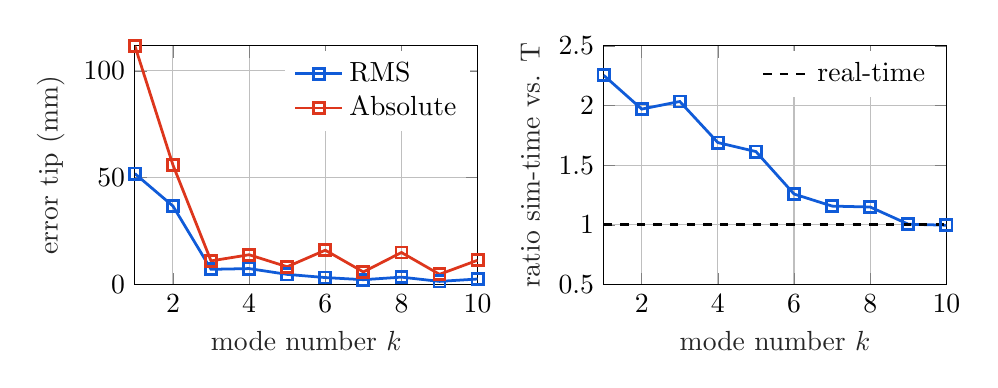
\begin{tikzpicture}

\begin{axis}[%
width=0.359\textwidth,
height=0.25\textwidth,
at={(0\textwidth,0\textwidth)},
scale only axis,
xmin=1,
xmax=10,
xlabel style={font=\color{white!15!black}},
xlabel={mode number $k$},
ymin=0,
ymax=111.696273768534,
ylabel style={font=\color{white!15!black}},
ylabel={error tip (mm)},
axis background/.style={fill=white},
xmajorgrids,
ymajorgrids,
legend style={legend cell align=left, align=left, draw=none}
]
\addplot [color=mycolor1, line width=1.0pt, mark=square, mark options={solid, mycolor1}]
  table[row sep=crcr]{%
1	51.8835913680113\\
2	36.716376998632\\
3	7.09768995463864\\
4	7.4468656014925\\
5	4.73611875774346\\
6	3.24570191666416\\
7	2.25205701458076\\
8	3.44519374750976\\
9	1.45285500840613\\
10	2.57094900354925\\
};
\addlegendentry{RMS}

\addplot [color=mycolor2, line width=1.0pt, mark=square, mark options={solid, mycolor2}]
  table[row sep=crcr]{%
1	111.696273768534\\
2	55.9315300451543\\
3	11.0399416681407\\
4	13.9183853058214\\
5	8.29890085334986\\
6	16.0490846650911\\
7	5.87384916377914\\
8	14.9842167697155\\
9	4.76901584170251\\
10	11.3462560434657\\
};
\addlegendentry{Absolute}

\end{axis}

\begin{axis}[%
width=0.359\textwidth,
height=0.25\textwidth,
at={(0.491\textwidth,0\textwidth)},
scale only axis,
xmin=1,
xmax=10,
xlabel style={font=\color{white!15!black}},
xlabel={mode number $k$},
ymin=0.5,
ymax=2.5,
ylabel style={font=\color{white!15!black}},
ylabel={ratio sim-time vs. T},
axis background/.style={fill=white},
xmajorgrids,
ymajorgrids,
legend style={legend cell align=left, align=left, draw=none}
]
\addplot [color=mycolor1, line width=1.0pt, mark=square, mark options={solid, mycolor1}, forget plot]
  table[row sep=crcr]{%
1	2.25337640286765\\
2	1.96991933180336\\
3	2.03336549439757\\
4	1.6891078723406\\
5	1.61360983075653\\
6	1.25800563334923\\
7	1.15685709691339\\
8	1.14922384294707\\
9	1.00516301985147\\
10	0.996875294389735\\
};
\addplot [color=black, dashed, line width=1.0pt]
  table[row sep=crcr]{%
1	1\\
10	1\\
};
\addlegendentry{real-time}

\end{axis}
\end{tikzpicture}% 
  \includegraphics*[width=\textwidth]{./pdf/thesis-figure-5-6.pdf}
  \caption{The benchmark results of the soft tentacle subjected to a tip-load for increasing model order $k$. (left) The root mean square error (RMSE) in (\ldatanum{Matlab1}{}) and absolute error in (\ldatanum{Matlab2}{}) for increasing $k$. Notice that the errors converge to an error band of about $3.25$ \si{\milli \meter}. (right) The ratio between CPU simulation time and finite horizon time (\ie, $T_{\textrm{cpu}}/T$) against the truncation order $k$, which shows all simulations achieve real-time computation. }
  %\vspace{-0.2cm}
  \label{fig:C3:EX2:mode_convergence_bench}
  \end{figure}
%   \clearpage
%  }
 
 Furthermore, we compare these simulation runs with a high-order mode of $k = 25$, where investigate the root mean square error, absolute error, and the ratio between actual CPU simulation time $T_{\textrm{sim}}$ and finite horizon $T$. The benchmark is shown in Figure \ref{fig:C3:EX2:mode_convergence_bench}. From these results, we observe that the solutions quickly converge to a narrow error band, namely for $k>3$ the difference in trajectories is near negligible. The RMS error is about $3.25$ \si{\milli \meter} or $2.7\%$ normalized by $L$.  Regarding computation time, we observe a linear decrease for a linear increase in modal order $k$. Note that for $k > 8$, the simulations are close to losing real-time performance. We therefore choose a modal basis of order $k = 8$. 
\end{example}

\begin{example}[Energy-based controller]
Following, we now subjected the soft robot to the proposed energy-based controller in \eqref{eq:C3:control}, where the control gains are tuned to produce a smooth transient: $\lambda_1 = 0.01$ and $\lambda_2 = 0.001$. The artificial spring stiffness is chosen as $\mat{k}_p = \blkdiag{0.01\cdot \mat{I}_3, \mat{I}_3}$. Lastly, the desired configuration of the end-effector is chosen as follows:
%
\begin{equation*}
\mat{g}_d = \begin{pmatrix} \mat{I}_3 & \mat{\gamma}_d \\ \vec{0}_3^\top & 1 \end{pmatrix} \quad \text{with} \quad \mat{\gamma}_d = \begin{pmatrix}  0.04 \\ 0.00 \\ -0.01  \end{pmatrix}.
\end{equation*}
%
The numerical results of the closed-loop system are shown in Figure \ref{fig:octarm1} and \ref{fig:octarm1_states}. It is worth mentioning that these simulation run at $\pm120$ \si{\hertz} real-time.$^{1}$ \blankfootnote{$^{1}$Real-time bandwidth is determined by the ratio between finite horizon and CPU's computation time, \ie, $f \approx T/T_{\textrm{sim}}$,which is affected most by spatial stepsize due to explicit integration.} 

Figure \ref{fig:octarm1} shows the evolution of the continuous deformation along the soft robotic body, whereas Figure \ref{fig:octarm1_states} shows the modal coefficients $\vec{q}(t)$ and generalized momenta $\vec{p}(t)$. As can be seen, the end-effector of the soft robot manipulator converges to the desired set-point $\mat{g}_d \in \SE{3}$. Although the control gains could be increased to promote a faster transient, it was observed that high gains lead to undesired (propagating) oscillations of the flexible structure. A possible solution might be to introduce negative damping to the controller Hamiltonian $\Hm_d$, to overcome the soft robot's structural damping.

For the second simulation run, we modified the control gains to highlight an interesting property of the proposed controller. To be more specific, we increase the controller gains to $\lambda_1 = \lambda_2 = 0.1$. The numerical results for the increased controller gains are shown in Figure \ref{fig:octarm2} and Figure \ref{fig:octarm2_states}. Although the control goal and the initial conditions are chosen identical, the soft robot converges to a different configuration -- albeit, a shape with less '\textit{complexity}'. The cause of less complicated bending patterns has two origins. First, increasing the control gains also artificially impacts the structural stiffness of the soft robot, resulting in soft robot with a higher perceived stiffness. Second, by increasing the stabilizing term $\lambda_2$ in the damped Jacobian inverse \eqref{eq:C3:jacob_damped}, more weight is given towards finding a solution that also minimizes the joint angles $\lVert \vec{q} \rVert_2 $.  This is to be expected, as intrinsically, it requires more energy to achieve higher-order modes deformations $\{\theta_n\}_{n=1}^k$ of the Legendre basis. Hence, the energy-based controller will thus find a minimizer that accounts for the ordering of the shape basis, penalizing higher-order modes. To some extent, the high intrinsic damping in soft robots acts as a spatial low filter which is beneficial for both modeling as control. This effect is not observed in classical semi-rigid robots.  This result indicates that the proposed controller can be effectively tuned alter the structural compliance of the soft robot; and thus could be implemented carefully to preserve '\textit{softness}'. 
\end{example}

\afterpage{
  \vfill
  \begin{figure*}[!t]
    \centering
    \vspace{-12mm}
    %% This file was created by matlab2tikz.
%
\begin{tikzpicture}

\begin{axis}[%
width=0.783\textwidth,
height=0.541\textwidth,
at={(0.121\textwidth,0\textwidth)},
scale only axis,
xmin=0,
xmax=1,
ymin=0,
ymax=1,
axis line style={draw=none},
ticks=none,
axis x line*=bottom,
axis y line*=left,
colorbar style={width=6,xshift=-7.5pt}
]
\end{axis}

\begin{axis}[%
width=0.31\textwidth,
height=0.149\textwidth,
at={(0\textwidth,0.413\textwidth)},
scale only axis,
axis on top,
xmin=0.5,
xmax=1024.5,
tick align=outside,
y dir=reverse,
ymin=0.5,
ymax=512.5,
axis line style={draw=none},
ticks=none,
colorbar style={width=6,xshift=-7.5pt}
]
\addplot [forget plot] graphics [xmin=0.5, xmax=1024.5, ymin=0.5, ymax=512.5] {fig_C3_3D_srmsoft-1.png};
\end{axis}

\begin{axis}[%
width=0.31\textwidth,
height=0.149\textwidth,
at={(0.34\textwidth,0.413\textwidth)},
scale only axis,
axis on top,
xmin=0.5,
xmax=1024.5,
tick align=outside,
y dir=reverse,
ymin=0.5,
ymax=512.5,
axis line style={draw=none},
ticks=none,
colorbar style={width=6,xshift=-7.5pt}
]
\addplot [forget plot] graphics [xmin=0.5, xmax=1024.5, ymin=0.5, ymax=512.5] {fig_C3_3D_srmsoft-2.png};
\end{axis}

\begin{axis}[%
width=0.31\textwidth,
height=0.149\textwidth,
at={(0.68\textwidth,0.413\textwidth)},
scale only axis,
axis on top,
xmin=0.5,
xmax=1024.5,
tick align=outside,
y dir=reverse,
ymin=0.5,
ymax=512.5,
axis line style={draw=none},
ticks=none,
colorbar style={width=6,xshift=-7.5pt}
]
\addplot [forget plot] graphics [xmin=0.5, xmax=1024.5, ymin=0.5, ymax=512.5] {fig_C3_3D_srmsoft-3.png};
\end{axis}

\begin{axis}[%
width=0.31\textwidth,
height=0.149\textwidth,
at={(0\textwidth,0.214\textwidth)},
scale only axis,
axis on top,
xmin=0.5,
xmax=1024.5,
tick align=outside,
y dir=reverse,
ymin=0.5,
ymax=512.5,
axis line style={draw=none},
ticks=none,
colorbar style={width=6,xshift=-7.5pt}
]
\addplot [forget plot] graphics [xmin=0.5, xmax=1024.5, ymin=0.5, ymax=512.5] {fig_C3_3D_srmsoft-4.png};
\end{axis}

\begin{axis}[%
width=0.31\textwidth,
height=0.149\textwidth,
at={(0.34\textwidth,0.214\textwidth)},
scale only axis,
axis on top,
xmin=0.5,
xmax=1024.5,
tick align=outside,
y dir=reverse,
ymin=0.5,
ymax=512.5,
axis line style={draw=none},
ticks=none,
colorbar style={width=6,xshift=-7.5pt}
]
\addplot [forget plot] graphics [xmin=0.5, xmax=1024.5, ymin=0.5, ymax=512.5] {fig_C3_3D_srmsoft-5.png};
\end{axis}

\begin{axis}[%
width=0.31\textwidth,
height=0.149\textwidth,
at={(0.68\textwidth,0.214\textwidth)},
scale only axis,
axis on top,
xmin=0.5,
xmax=1024.5,
tick align=outside,
y dir=reverse,
ymin=0.5,
ymax=512.5,
axis line style={draw=none},
ticks=none,
colorbar style={width=6,xshift=-7.5pt}
]
\addplot [forget plot] graphics [xmin=0.5, xmax=1024.5, ymin=0.5, ymax=512.5] {fig_C3_3D_srmsoft-6.png};
\end{axis}

\begin{axis}[%
width=0.31\textwidth,
height=0.149\textwidth,
at={(0\textwidth,0.015\textwidth)},
scale only axis,
axis on top,
xmin=0.5,
xmax=1024.5,
tick align=outside,
y dir=reverse,
ymin=0.5,
ymax=512.5,
axis line style={draw=none},
ticks=none,
colorbar style={width=6,xshift=-7.5pt}
]
\addplot [forget plot] graphics [xmin=0.5, xmax=1024.5, ymin=0.5, ymax=512.5] {fig_C3_3D_srmsoft-7.png};
\end{axis}

\begin{axis}[%
width=0.31\textwidth,
height=0.149\textwidth,
at={(0.34\textwidth,0.015\textwidth)},
scale only axis,
axis on top,
xmin=0.5,
xmax=1024.5,
tick align=outside,
y dir=reverse,
ymin=0.5,
ymax=512.5,
axis line style={draw=none},
ticks=none,
colorbar style={width=6,xshift=-7.5pt}
]
\addplot [forget plot] graphics [xmin=0.5, xmax=1024.5, ymin=0.5, ymax=512.5] {fig_C3_3D_srmsoft-8.png};
\end{axis}

\begin{axis}[%
width=0.31\textwidth,
height=0.149\textwidth,
at={(0.68\textwidth,0.015\textwidth)},
scale only axis,
axis on top,
xmin=0.5,
xmax=1024.5,
tick align=outside,
y dir=reverse,
ymin=0.5,
ymax=512.5,
axis line style={draw=none},
ticks=none,
colorbar style={width=6,xshift=-7.5pt}
]
\addplot [forget plot] graphics [xmin=0.5, xmax=1024.5, ymin=0.5, ymax=512.5] {fig_C3_3D_srmsoft-9.png};
\end{axis}
\end{tikzpicture}%
    \includegraphics*[width=\textwidth]{./pdf/thesis-figure-5-7.pdf}
    \vspace{-1mm}
    \caption{Three-dimensional evolution of the soft robot manipulators, converging to the desired set-point $g_d \in \SE{3}$ (indicated by the pink ball). Observe that the morphological motion that arises due to the energy-based controller has a close similarity to those an octopus' tentacle. }
    \label{fig:octarm1}
  \end{figure*}
  \vspace{2mm}
  \begin{figure}[!t]
    \centering
    \vspace{-20mm}
    %% This file was created by matlab2tikz.
%
\definecolor{mycolor1}{rgb}{0.00000,0.34510,0.65882}%
\definecolor{mycolor2}{rgb}{0.79216,0.11765,0.17255}%
\definecolor{mycolor3}{rgb}{0.20392,0.65490,0.24706}%
\definecolor{mycolor4}{rgb}{0.93333,0.43922,0.13725}%
\definecolor{mycolor5}{rgb}{0.49412,0.14510,0.51373}%
\definecolor{mycolor6}{rgb}{0.97647,0.67059,0.08235}%
\definecolor{mycolor7}{rgb}{0.24314,0.18039,0.52549}%
\definecolor{mycolor8}{rgb}{0.71373,0.81961,0.14118}%
%
\begin{tikzpicture}

\begin{axis}[%
width=0.37\textwidth,
height=0.3\textwidth,
at={(0\textwidth,0\textwidth)},
scale only axis,
xmin=0,
xmax=6,
xlabel style={font=\color{white!15!black}},
xlabel={time (s)},
ymin=-0.08,
ymax=0.05,
ylabel style={font=\color{white!15!black}},
ylabel={$\vec{q}(t)$},
axis background/.style={fill=white},
xmajorgrids,
ymajorgrids,
ylabel style={yshift=-9.5pt}
]
\addplot [color=mycolor1, line width=1.5pt, forget plot]
  table[row sep=crcr]{%
0	0.00100000000000033\\
0.0999999999999996	0.000732535763058095\\
0.2	0.000833074040049731\\
0.983333333333333	0.00293974513825557\\
1.88333333333333	0.00385980750118531\\
3.56666666666667	0.00456401284455943\\
5.98333333333333	0.00467530988040199\\
};
\addplot [color=mycolor2, line width=1.5pt, forget plot]
  table[row sep=crcr]{%
0	0.00100000000000033\\
0.0666666666666664	0.000815426863866264\\
0.166666666666667	2.29049321793795e-05\\
0.533333333333333	-0.000711551703824753\\
1.08333333333333	-0.000502410285309729\\
2.2	0.000837531682200243\\
4.61666666666667	0.00391868974278786\\
5.98333333333333	0.00474301868188931\\
};
\addplot [color=mycolor3, line width=1.5pt, forget plot]
  table[row sep=crcr]{%
0	0.00100000000000033\\
0.0499999999999998	0.000862540745709239\\
0.083333333333333	7.9715738317887e-05\\
0.15	-0.00286500293669523\\
0.566666666666666	-0.023039392105896\\
0.7	-0.0277099330252577\\
0.85	-0.0319308929707871\\
1.03333333333333	-0.0360781551803369\\
1.25	-0.0399905513472296\\
1.51666666666667	-0.0437716260847507\\
1.83333333333333	-0.0472059644891329\\
2.2	-0.0501605291248053\\
2.63333333333333	-0.0526554477870347\\
3.16666666666667	-0.0547181046207754\\
3.85	-0.0563324704569999\\
4.78333333333333	-0.0575004877876975\\
5.98333333333333	-0.0581824435438563\\
};
\addplot [color=mycolor4, line width=1.5pt, forget plot]
  table[row sep=crcr]{%
0	0.00100000000000033\\
0.116666666666666	0.00141810417547372\\
0.283333333333333	0.00284520823013867\\
0.6	0.00442456639570743\\
1.05	0.00557974262121252\\
1.78333333333333	0.00638962866368331\\
3	0.00663203285105141\\
5.98333333333333	0.00622013713842939\\
};
\addplot [color=mycolor5, line width=1.5pt, forget plot]
  table[row sep=crcr]{%
0	0.00100000000000033\\
0.116666666666666	0.00120378091308915\\
0.7	0.00750897575729681\\
1.03333333333333	0.00941072600012749\\
1.53333333333333	0.0112112704692127\\
2.23333333333333	0.012708719652073\\
3.23333333333333	0.0138286419884883\\
4.78333333333333	0.0145243875181809\\
5.98333333333333	0.014719913864214\\
};
\addplot [color=mycolor6, line width=1.5pt, forget plot]
  table[row sep=crcr]{%
0	0.00100000000000033\\
0.0333333333333332	0.000198168650838326\\
0.15	-0.000146438128797222\\
0.5	-0.00135936491615585\\
1.21666666666667	-0.00436997869578892\\
1.93333333333333	-0.00624567310612001\\
2.91666666666667	-0.00777048401753788\\
4.25	-0.00880789873058863\\
5.98333333333333	-0.00933423162050939\\
};
\addplot [color=mycolor7, line width=1.5pt, forget plot]
  table[row sep=crcr]{%
0	0.00100000000000033\\
0.0333333333333332	0.000156244427058638\\
0.116666666666666	5.79230952633125e-05\\
0.383333333333334	0.000943852594205374\\
1.13333333333333	0.00334768860949186\\
1.9	0.0045178578491134\\
3	0.00516635855243219\\
5.18333333333333	0.00529648809347449\\
5.98333333333333	0.00527621146404211\\
};
\addplot [color=mycolor8, line width=1.5pt, forget plot]
  table[row sep=crcr]{%
0	0.00100000000000033\\
0.0333333333333332	0.000202593966617037\\
0.133333333333334	-0.000139925918890782\\
0.633333333333334	-0.000290741139219897\\
2.43333333333333	0.000544582580761066\\
5.4	0.00102824900177723\\
5.98333333333333	0.00105769909447329\\
};
\end{axis}

\begin{axis}[%
width=0.362\textwidth,
height=0.283\textwidth,
at={(0.493\textwidth,0.017\textwidth)},
scale only axis,
xmin=0,
xmax=6,
xlabel style={font=\color{white!15!black}},
xlabel={time (s)},
ymin=-0.35,
ymax=0.25,
ylabel style={font=\color{white!15!black}},
ylabel={$\vec{p}(t)$},
axis background/.style={fill=white},
xmajorgrids,
ymajorgrids,
ylabel style={yshift=-9.5pt}
]
\addplot [color=mycolor1, line width=1.5pt, forget plot]
  table[row sep=crcr]{%
0	0\\
0.0166666666666666	-0.0022389882244136\\
0.0333333333333332	-0.000883339665332272\\
0.0499999999999998	0.00341285410763525\\
0.083333333333333	0.0209682250607592\\
0.0999999999999996	0.0299272242976309\\
0.116666666666666	0.0363007852376453\\
0.15	0.0415904232953528\\
0.2	0.0426646798081922\\
0.25	0.0431498198932294\\
0.35	0.0534566241726644\\
0.45	0.0695610657130628\\
0.516666666666667	0.0783721351837778\\
0.6	0.0840852512352104\\
0.683333333333334	0.0863756086052616\\
0.95	0.082181744318417\\
1.06666666666667	0.0775254662450982\\
1.15	0.0745111915692922\\
1.23333333333333	0.0705074658301132\\
1.31666666666667	0.0671763307110664\\
1.43333333333333	0.0615429950795159\\
1.55	0.056630179496759\\
1.66666666666667	0.0511707264730568\\
1.81666666666667	0.045058649382578\\
1.96666666666667	0.0387539192842397\\
2.15	0.0320747958970502\\
2.33333333333333	0.0256257407205949\\
2.68333333333333	0.0155973583919842\\
2.93333333333333	0.00968324432571865\\
3.9	-0.00282964760215965\\
5.01666666666667	-0.00508088103279025\\
5.98333333333333	-0.00363870056156568\\
};
\addplot [color=mycolor2, line width=1.5pt, forget plot]
  table[row sep=crcr]{%
0	0\\
0.0166666666666666	9.43487233691087e-05\\
0.0333333333333332	0.00374222577773953\\
0.0499999999999998	0.0116403389419908\\
0.0666666666666664	0.0249326558468956\\
0.0999999999999996	0.0602875600306225\\
0.116666666666666	0.0754236442710443\\
0.15	0.0946616837032153\\
0.2	0.109267109516779\\
0.25	0.12031478286272\\
0.333333333333333	0.134294774828271\\
0.383333333333334	0.141856581716694\\
0.483333333333333	0.149327112540067\\
0.55	0.147622555565285\\
0.683333333333334	0.135855342230123\\
1.03333333333333	0.106290025946391\\
1.16666666666667	0.0973187930340149\\
1.31666666666667	0.0881915763168086\\
2.15	0.0544228064321208\\
3.3	0.0316672329332013\\
3.86666666666667	0.024388442678271\\
4.61666666666667	0.0167435708339321\\
5.98333333333333	0.00765324475762874\\
};
\addplot [color=mycolor3, line width=1.5pt, forget plot]
  table[row sep=crcr]{%
0	0\\
0.0333333333333332	-0.00601773126125504\\
0.0499999999999998	-0.0175035933402601\\
0.0666666666666664	-0.0403285481139068\\
0.0999999999999996	-0.0957554871255155\\
0.116666666666666	-0.115582672571266\\
0.133333333333334	-0.129906392359716\\
0.166666666666667	-0.146413506962633\\
0.45	-0.234446920538813\\
0.5	-0.243974849565285\\
0.55	-0.247085215228163\\
0.6	-0.246170440825747\\
0.7	-0.238372173543493\\
0.966666666666667	-0.207851034477204\\
1.26666666666667	-0.173275120450096\\
1.53333333333333	-0.145645737710617\\
1.81666666666667	-0.120153280842121\\
2.11666666666667	-0.0974720261209265\\
2.43333333333333	-0.0778494014631992\\
2.81666666666667	-0.0591368039190385\\
3.18333333333333	-0.0453590409972904\\
3.6	-0.033491017145419\\
4.21666666666667	-0.0214186747916214\\
4.8	-0.0140850467474376\\
5.85	-0.00680601249895663\\
5.98333333333333	-0.00622017634046035\\
};
\addplot [color=mycolor4, line width=1.5pt, forget plot]
  table[row sep=crcr]{%
0	0\\
0.0166666666666666	0.00429541078256879\\
0.0333333333333332	0.00263804163440362\\
0.0499999999999998	0.00454590376245179\\
0.116666666666666	0.0210669059432442\\
0.4	0.037309133342168\\
0.5	0.0428483501169445\\
0.6	0.0440376490896828\\
0.783333333333333	0.041890563901938\\
2.5	0.0119629161241201\\
3.26666666666667	0.00582623526262172\\
4.2	0.00224211894312276\\
5.51666666666667	0.000582252719429022\\
5.98333333333333	0.000382688812645249\\
};
\addplot [color=mycolor5, line width=1.5pt, forget plot]
  table[row sep=crcr]{%
0	0\\
0.0166666666666666	0.00210925592747824\\
0.0333333333333332	0.000311438389804408\\
0.0999999999999996	0.013085153903047\\
0.133333333333334	0.0179716480615415\\
0.516666666666667	0.0511382326573706\\
0.633333333333334	0.0540311437642016\\
0.8	0.0530108149606079\\
1.11666666666667	0.0464776135586984\\
2.1	0.0251201124650873\\
2.7	0.0163663308070259\\
3.38333333333333	0.00981924236202847\\
4.61666666666667	0.00383154595069701\\
5.98333333333333	0.00141991166409738\\
};
\addplot [color=mycolor6, line width=1.5pt, forget plot]
  table[row sep=crcr]{%
0	0\\
0.0166666666666666	-0.00217007321632678\\
0.0333333333333332	-0.000185607572342761\\
0.0999999999999996	-0.00158054834730414\\
0.183333333333334	-0.00225648059750316\\
0.266666666666667	-0.00390375806547461\\
0.533333333333333	-0.0126560725221205\\
0.683333333333334	-0.0142168277707135\\
1.66666666666667	-0.00863922636016667\\
4.28333333333333	-0.000133565213567444\\
5.98333333333333	0.000159970381544916\\
};
\addplot [color=mycolor7, line width=1.5pt, forget plot]
  table[row sep=crcr]{%
0	0\\
0.0166666666666666	-0.00167429747212822\\
0.0333333333333332	0.000395387159262128\\
0.0499999999999998	-0.000951895314057261\\
0.0666666666666664	1.12957230911093e-05\\
0.116666666666666	-0.00177407886396708\\
0.166666666666667	-0.00146491844196017\\
0.25	-0.00261097687383671\\
0.333333333333333	-0.00335107132516743\\
0.483333333333333	-0.0057424492321605\\
1.16666666666667	-0.00728877674664208\\
5.98333333333333	-0.000527173648784185\\
};
\addplot [color=mycolor8, line width=1.5pt, forget plot]
  table[row sep=crcr]{%
0	0\\
0.266666666666667	0.000609282752626505\\
0.35	0.000576844080265815\\
0.466666666666667	0.00151396580232976\\
0.583333333333333	0.00166954783330731\\
0.7	0.00219246632700187\\
0.85	0.00211800244887694\\
1.03333333333333	0.00230016187960302\\
1.31666666666667	0.00199878873634241\\
1.73333333333333	0.00159964014130232\\
2.65	0.000559782632032935\\
5.98333333333333	-0.000139371173606406\\
};
\end{axis}
\end{tikzpicture}%
    \includegraphics*[width=\textwidth]{./pdf/thesis-figure-5-8.pdf}
    \caption{The evolution of the modal coefficients and the generalized momenta of the soft robot manipulator. The modal coefficients $\q$ are ordered as follows: $k \in \{\ldatanum{Matlab1}{1},\ldatanum{Matlab2}{2},\ldatanum{Matlab3}{3},\ldatanum{Matlab4}{4},\ldatanum{Matlab5}{5},\ldatanum{Matlab6}{6},\ldatanum{Matlab7}{7},\ldatanum{Matlab8}{8}\}$. Observe that mainly mode 3 is dominant. \label{fig:octarm1_states}}
  \end{figure}
  \clearpage
}

\afterpage{
  \vfill
  \begin{figure*}[!t]
    \centering
    %% This file was created by matlab2tikz.
%
\begin{tikzpicture}

\begin{axis}[%
width=0.783\textwidth,
height=0.541\textwidth,
at={(0.121\textwidth,0\textwidth)},
scale only axis,
xmin=0,
xmax=1,
ymin=0,
ymax=1,
axis line style={draw=none},
ticks=none,
axis x line*=bottom,
axis y line*=left,
colorbar style={width=6,xshift=-7.5pt}
]
\end{axis}

\begin{axis}[%
width=0.31\textwidth,
height=0.132\textwidth,
at={(0\textwidth,0.422\textwidth)},
scale only axis,
axis on top,
xmin=0.5,
xmax=1034.5,
tick align=outside,
y dir=reverse,
ymin=0.5,
ymax=458.5,
axis line style={draw=none},
ticks=none,
colorbar style={width=6,xshift=-7.5pt}
]
\addplot [forget plot] graphics [xmin=0.5, xmax=1034.5, ymin=0.5, ymax=458.5] {./fig/fig_C3_3D_srmstiff-1.png};
\end{axis}

\begin{axis}[%
width=0.31\textwidth,
height=0.132\textwidth,
at={(0.34\textwidth,0.422\textwidth)},
scale only axis,
axis on top,
xmin=0.5,
xmax=1034.5,
tick align=outside,
y dir=reverse,
ymin=0.5,
ymax=458.5,
axis line style={draw=none},
ticks=none,
colorbar style={width=6,xshift=-7.5pt}
]
\addplot [forget plot] graphics [xmin=0.5, xmax=1034.5, ymin=0.5, ymax=458.5] {./fig/fig_C3_3D_srmstiff-2.png};
\end{axis}

\begin{axis}[%
width=0.31\textwidth,
height=0.132\textwidth,
at={(0.68\textwidth,0.422\textwidth)},
scale only axis,
axis on top,
xmin=0.5,
xmax=1034.5,
tick align=outside,
y dir=reverse,
ymin=0.5,
ymax=458.5,
axis line style={draw=none},
ticks=none,
colorbar style={width=6,xshift=-7.5pt}
]
\addplot [forget plot] graphics [xmin=0.5, xmax=1034.5, ymin=0.5, ymax=458.5] {./fig/fig_C3_3D_srmstiff-3.png};
\end{axis}

\begin{axis}[%
width=0.31\textwidth,
height=0.132\textwidth,
at={(0\textwidth,0.223\textwidth)},
scale only axis,
axis on top,
xmin=0.5,
xmax=1034.5,
tick align=outside,
y dir=reverse,
ymin=0.5,
ymax=458.5,
axis line style={draw=none},
ticks=none,
colorbar style={width=6,xshift=-7.5pt}
]
\addplot [forget plot] graphics [xmin=0.5, xmax=1034.5, ymin=0.5, ymax=458.5] {./fig/fig_C3_3D_srmstiff-4.png};
\end{axis}

\begin{axis}[%
width=0.31\textwidth,
height=0.132\textwidth,
at={(0.34\textwidth,0.223\textwidth)},
scale only axis,
axis on top,
xmin=0.5,
xmax=1034.5,
tick align=outside,
y dir=reverse,
ymin=0.5,
ymax=458.5,
axis line style={draw=none},
ticks=none,
colorbar style={width=6,xshift=-7.5pt}
]
\addplot [forget plot] graphics [xmin=0.5, xmax=1034.5, ymin=0.5, ymax=458.5] {./fig/fig_C3_3D_srmstiff-5.png};
\end{axis}

\begin{axis}[%
width=0.31\textwidth,
height=0.132\textwidth,
at={(0.68\textwidth,0.223\textwidth)},
scale only axis,
axis on top,
xmin=0.5,
xmax=1034.5,
tick align=outside,
y dir=reverse,
ymin=0.5,
ymax=458.5,
axis line style={draw=none},
ticks=none,
colorbar style={width=6,xshift=-7.5pt}
]
\addplot [forget plot] graphics [xmin=0.5, xmax=1034.5, ymin=0.5, ymax=458.5] {./fig/fig_C3_3D_srmstiff-6.png};
\end{axis}

\begin{axis}[%
width=0.31\textwidth,
height=0.132\textwidth,
at={(0\textwidth,0.024\textwidth)},
scale only axis,
axis on top,
xmin=0.5,
xmax=1034.5,
tick align=outside,
y dir=reverse,
ymin=0.5,
ymax=458.5,
axis line style={draw=none},
ticks=none,
colorbar style={width=6,xshift=-7.5pt}
]
\addplot [forget plot] graphics [xmin=0.5, xmax=1034.5, ymin=0.5, ymax=458.5] {./fig/fig_C3_3D_srmstiff-7.png};
\end{axis}

\begin{axis}[%
width=0.31\textwidth,
height=0.132\textwidth,
at={(0.34\textwidth,0.024\textwidth)},
scale only axis,
axis on top,
xmin=0.5,
xmax=1034.5,
tick align=outside,
y dir=reverse,
ymin=0.5,
ymax=458.5,
axis line style={draw=none},
ticks=none,
colorbar style={width=6,xshift=-7.5pt}
]
\addplot [forget plot] graphics [xmin=0.5, xmax=1034.5, ymin=0.5, ymax=458.5] {./fig/fig_C3_3D_srmstiff-8.png};
\end{axis}

\begin{axis}[%
width=0.31\textwidth,
height=0.132\textwidth,
at={(0.68\textwidth,0.024\textwidth)},
scale only axis,
axis on top,
xmin=0.5,
xmax=1034.5,
tick align=outside,
y dir=reverse,
ymin=0.5,
ymax=458.5,
axis line style={draw=none},
ticks=none,
colorbar style={width=6,xshift=-7.5pt}
]
\addplot [forget plot] graphics [xmin=0.5, xmax=1034.5, ymin=0.5, ymax=458.5] {./fig/fig_C3_3D_srmstiff-9.png};
\end{axis}
\end{tikzpicture}%
    \includegraphics*[width=\textwidth]{./pdf/thesis-figure-5-9.pdf}
    \vspace{-1mm}
    \caption{Three-dimensional evolution of the soft robot manipulators, converging to the desired set-point $g_d \in \SE{3}$ (indicated by the pink ball). Observe that a different morphology arises due to higher control gains, \ie, $\lambda_1 = \lambda_2 = 0.1$, which is caused by the controller affecting the structural compliance of the soft robot.}
    \label{fig:octarm2}
\end{figure*}
\vspace{2mm}
  \begin{figure}[!t]
    \centering
    %% This file was created by matlab2tikz.
%
\definecolor{mycolor1}{rgb}{0.00000,0.34510,0.65882}%
\definecolor{mycolor2}{rgb}{0.79216,0.11765,0.17255}%
\definecolor{mycolor3}{rgb}{0.20392,0.65490,0.24706}%
\definecolor{mycolor4}{rgb}{0.93333,0.43922,0.13725}%
\definecolor{mycolor5}{rgb}{0.49412,0.14510,0.51373}%
\definecolor{mycolor6}{rgb}{0.97647,0.67059,0.08235}%
\definecolor{mycolor7}{rgb}{0.24314,0.18039,0.52549}%
\definecolor{mycolor8}{rgb}{0.71373,0.81961,0.14118}%
%
\begin{tikzpicture}

\begin{axis}[%
width=0.37\textwidth,
height=0.3\textwidth,
at={(0\textwidth,0\textwidth)},
scale only axis,
xmin=0,
xmax=6,
xlabel style={font=\color{white!15!black}},
xlabel={time (s)},
ymin=-0.03,
ymax=0.03,
ylabel style={font=\color{white!15!black}},
ylabel={$\vec{q}(t)$},
axis background/.style={fill=white},
xmajorgrids,
ymajorgrids,
ylabel style={yshift=-9.5pt}
]
\addplot [color=mycolor1, line width=1.5pt, forget plot]
  table[row sep=crcr]{%
0	0.00100000000000033\\
0.0999999999999996	0.00103971588713581\\
0.266666666666667	0.00117549874542888\\
0.383333333333334	0.00151761804318351\\
0.466666666666667	0.0020321988385863\\
0.533333333333333	0.00269484033943268\\
0.6	0.00362287778731041\\
0.666666666666667	0.00480943290937663\\
0.783333333333333	0.00723888784369642\\
0.916666666666667	0.00993813998401816\\
1.01666666666667	0.0116933716352383\\
1.13333333333333	0.0134396186381096\\
1.25	0.0149055578394517\\
1.38333333333333	0.0162993751876677\\
1.53333333333333	0.0175773864308324\\
1.7	0.0187122624033087\\
1.9	0.0197705971571311\\
2.13333333333333	0.0206997678583969\\
2.41666666666667	0.0215278097919391\\
2.78333333333333	0.0222971077704228\\
3.26666666666667	0.0230159563690266\\
3.88333333333333	0.0236495932052421\\
4.61666666666667	0.024112682295744\\
5.46666666666667	0.0243539007222431\\
5.98333333333333	0.0243980090290519\\
};
\addplot [color=mycolor2, line width=1.5pt, forget plot]
  table[row sep=crcr]{%
0	0.00100000000000033\\
0.0666666666666664	0.00105311655584384\\
0.233333333333333	0.00116843807874023\\
0.35	0.00147420323991021\\
0.433333333333334	0.00194860524107288\\
0.5	0.00257916654293755\\
0.566666666666666	0.00350000523156258\\
0.633333333333334	0.00473113614920528\\
0.716666666666667	0.00661780995214567\\
0.9	0.0109615584895115\\
1	0.0129998877149839\\
1.1	0.0147580713623414\\
1.21666666666667	0.0165032287013416\\
1.33333333333333	0.0179768873443331\\
1.46666666666667	0.0193905577530034\\
1.61666666666667	0.0207013978604067\\
1.78333333333333	0.0218775033025445\\
1.96666666666667	0.0228957542957406\\
2.18333333333333	0.0238008789240363\\
2.41666666666667	0.0244890740303729\\
2.68333333333333	0.0249949024252842\\
3	0.0253104501963675\\
3.4	0.0254202569265454\\
4.03333333333333	0.0252824430513252\\
5.51666666666667	0.0249299723896934\\
5.98333333333333	0.0249147141724686\\
};
\addplot [color=mycolor3, line width=1.5pt, forget plot]
  table[row sep=crcr]{%
0	0.00100000000000033\\
0.0666666666666664	0.00102726510297035\\
0.366666666666666	0.000737642414384787\\
0.466666666666667	0.000278847250939407\\
0.533333333333333	-0.000281141456603962\\
0.6	-0.00111083686174762\\
0.666666666666667	-0.002225366175443\\
0.75	-0.00393278505075312\\
0.983333333333333	-0.00890343295805085\\
1.1	-0.0109910669020881\\
1.21666666666667	-0.0127832956910714\\
1.35	-0.0145210133303681\\
1.48333333333333	-0.0159829379758865\\
1.63333333333333	-0.0173562015267317\\
1.8	-0.0186066577840558\\
1.98333333333333	-0.0197124488095266\\
2.2	-0.0207327031007214\\
2.45	-0.0216144159348701\\
2.73333333333333	-0.0223303434251818\\
3.08333333333333	-0.0229181177611375\\
3.5	-0.0233304403725221\\
4.06666666666667	-0.0235919785806953\\
5	-0.023692463835169\\
5.98333333333333	-0.0236837306927438\\
};
\addplot [color=mycolor4, line width=1.5pt, forget plot]
  table[row sep=crcr]{%
0	0.00100000000000033\\
0.35	0.00108931508857779\\
0.483333333333333	0.0008990318734865\\
0.583333333333333	0.000528675970282499\\
0.716666666666667	-0.000277596521174317\\
0.933333333333334	-0.00161510792239294\\
1.11666666666667	-0.00244992502715924\\
1.35	-0.00321670490910098\\
1.63333333333333	-0.00385664825599008\\
1.98333333333333	-0.00435911114960952\\
2.41666666666667	-0.00469427494522368\\
2.98333333333333	-0.00484612622651159\\
4	-0.00480169154302956\\
5.98333333333333	-0.00473770360391157\\
};
\addplot [color=mycolor5, line width=1.5pt, forget plot]
  table[row sep=crcr]{%
0	0.00100000000000033\\
0.083333333333333	0.000994901314072649\\
0.65	0.00126767572963615\\
0.883333333333334	0.00185079932096599\\
1.26666666666667	0.00277363851663992\\
1.65	0.00340005661597242\\
2.15	0.00391672489961614\\
2.83333333333333	0.00431760713006302\\
3.73333333333333	0.00456147046419542\\
5.08333333333333	0.00463591201961755\\
5.98333333333333	0.00462512633114986\\
};
\addplot [color=mycolor6, line width=1.5pt, forget plot]
  table[row sep=crcr]{%
0	0.00100000000000033\\
0.0166666666666666	0.000500185575834422\\
0.0333333333333332	0.000197547747774252\\
0.0666666666666664	-7.3172755499229e-07\\
0.216666666666667	-5.88301115236334e-05\\
0.666666666666667	-0.000294607243819023\\
0.833333333333333	-0.000692236559280524\\
1.2	-0.00194720527996939\\
1.56666666666667	-0.00300107480083689\\
1.93333333333333	-0.00374046675046369\\
2.35	-0.00427927455758859\\
2.85	-0.00463739001026742\\
3.5	-0.00482104718696696\\
4.76666666666667	-0.00482601613888356\\
5.98333333333333	-0.00479599395600161\\
};
\addplot [color=mycolor7, line width=1.5pt, forget plot]
  table[row sep=crcr]{%
0	0.00100000000000033\\
0.0166666666666666	0.0004659622024068\\
0.0333333333333332	0.000153422015163329\\
0.083333333333333	-6.44661669113589e-05\\
0.166666666666667	-0.00010673031102737\\
1.18333333333333	0.000282931758941452\\
2.46666666666667	0.000616973307469237\\
4.98333333333333	0.000962495013447473\\
5.98333333333333	0.000985388099384643\\
};
\addplot [color=mycolor8, line width=1.5pt, forget plot]
  table[row sep=crcr]{%
0	0.00100000000000033\\
0.0166666666666666	0.000466455293326895\\
0.0499999999999998	6.95620327464397e-05\\
0.0999999999999996	-5.22169375170023e-05\\
1.4	-0.000229871689484185\\
2.4	0.000103617059704852\\
3.65	0.000269590345438608\\
5.98333333333333	0.000312306373604798\\
};
\end{axis}

\begin{axis}[%
width=0.37\textwidth,
height=0.3\textwidth,
at={(0.486\textwidth,0\textwidth)},
scale only axis,
xmin=0,
xmax=6,
xlabel style={font=\color{white!15!black}},
xlabel={time (s)},
ymin=-0.2,
ymax=0.2,
ylabel style={font=\color{white!15!black}},
ylabel={$\vec{p}(t)$},
axis background/.style={fill=white},
xmajorgrids,
ymajorgrids,
ylabel style={yshift=-9.5pt}
]
\addplot [color=mycolor1, line width=1.5pt, forget plot]
  table[row sep=crcr]{%
0	0\\
0.0166666666666666	-0.0022389882244136\\
0.183333333333334	0.000434866614895668\\
0.233333333333333	0.00267622205121754\\
0.383333333333334	0.013520859814288\\
0.55	0.0257089047544286\\
0.633333333333334	0.0282938004675897\\
0.683333333333334	0.0287875600668777\\
0.816666666666666	0.025605003747418\\
0.833333333333333	0.0242842044133047\\
0.85	0.0241586353998642\\
0.866666666666667	0.0226830625412795\\
0.883333333333334	0.0225356119121836\\
0.9	0.0209329065210273\\
0.916666666666667	0.0207639502344037\\
0.933333333333334	0.0190596793306197\\
0.95	0.0188692384169205\\
0.966666666666667	0.0170875256387237\\
0.983333333333333	0.0168768205431524\\
1	0.0150405890505487\\
1.01666666666667	0.0148125355851256\\
1.03333333333333	0.0129434729821414\\
1.05	0.0127025741342122\\
1.06666666666667	0.0108209756296889\\
1.08333333333333	0.0105729492731799\\
1.1	0.00869754730816563\\
1.11666666666667	0.00844888956317913\\
1.13333333333333	0.00659672332693084\\
1.15	0.00635430488985644\\
1.16666666666667	0.00454064648885133\\
1.18333333333333	0.00431137887164645\\
1.2	0.00254971392038339\\
1.21666666666667	0.0023402918562514\\
1.23333333333333	0.00064234470140434\\
1.25	0.000459057606719604\\
1.26666666666667	-0.00116515013692098\\
1.28333333333333	-0.00131654912380075\\
1.3	-0.00285861694990164\\
1.31666666666667	-0.00297299606943646\\
1.33333333333333	-0.00442604813457592\\
1.35	-0.00449894654523764\\
1.36666666666667	-0.00585752669089157\\
1.38333333333333	-0.00588517691677648\\
1.4	-0.00714513974805442\\
1.41666666666667	-0.00712446973926806\\
1.43333333333333	-0.00828287102535263\\
1.45	-0.00821149105984276\\
1.46666666666667	-0.0092664797156754\\
1.48333333333333	-0.00914265816607873\\
1.5	-0.0100933713440314\\
1.51666666666667	-0.00991600241108692\\
1.53333333333333	-0.0107624647065432\\
1.55	-0.0105310305115021\\
1.56666666666667	-0.0112740579197776\\
1.61666666666667	-0.011290718295851\\
1.63333333333333	-0.0118320402515728\\
1.68333333333333	-0.0114421280337487\\
1.71666666666667	-0.0113003617875824\\
1.76666666666667	-0.0111939379552348\\
1.81666666666667	-0.0100739108464483\\
1.86666666666667	-0.00935895126453179\\
1.91666666666667	-0.00779004418847684\\
1.96666666666667	-0.00657421975455552\\
2.05	-0.00345689570505847\\
2.1	-0.00174977864537862\\
2.18333333333333	0.00188409444892379\\
2.26666666666667	0.00536794068727708\\
2.38333333333333	0.0107480901412398\\
2.53333333333333	0.0172614319530853\\
2.66666666666667	0.0227161695361202\\
2.81666666666667	0.0281200983205947\\
3.08333333333333	0.0350551958963763\\
3.3	0.038085098333922\\
3.5	0.0389356102112686\\
3.71666666666667	0.038014542137784\\
3.96666666666667	0.0351085583814195\\
4.33333333333333	0.0285572192478494\\
5.26666666666667	0.0100959336076532\\
5.63333333333333	0.00474042999280577\\
5.98333333333333	0.00107451489122834\\
};
\addplot [color=mycolor2, line width=1.5pt, forget plot]
  table[row sep=crcr]{%
0	0\\
0.0166666666666666	9.43487233691087e-05\\
0.0499999999999998	0.00266323847031824\\
0.133333333333334	0.00280950270942704\\
0.183333333333334	0.00363352539983275\\
0.233333333333333	0.00431271697322888\\
0.333333333333333	0.00898670336919949\\
0.383333333333334	0.0142021134234129\\
0.416666666666667	0.0192235705032076\\
0.45	0.0259051811251076\\
0.483333333333333	0.0344165857590815\\
0.516666666666667	0.0446711877554824\\
0.55	0.0564621974876767\\
0.583333333333333	0.0697305374431041\\
0.633333333333334	0.0915504870637092\\
0.7	0.1207082357883\\
0.75	0.139429964740127\\
0.766666666666667	0.145202684774989\\
0.816666666666666	0.158734055580934\\
0.833333333333333	0.162944497895182\\
0.9	0.174463512162525\\
1	0.182934740535887\\
1.01666666666667	0.182945448741529\\
1.03333333333333	0.183992555391628\\
1.05	0.183637921260007\\
1.06666666666667	0.184355786445977\\
1.08333333333333	0.183686939703855\\
1.1	0.184112453280627\\
1.11666666666667	0.183172704097718\\
1.13333333333333	0.183337350932957\\
1.15	0.182163487216103\\
1.16666666666667	0.182094332217769\\
1.18333333333333	0.180717742134026\\
1.2	0.180438249911181\\
1.21666666666667	0.178885859462361\\
1.23333333333333	0.178416559315981\\
1.25	0.176711601665145\\
1.26666666666667	0.176070620116452\\
1.28333333333333	0.174233261817895\\
1.3	0.173436746578419\\
1.31666666666667	0.171484596162736\\
1.33333333333333	0.170547053183263\\
1.35	0.168495574661459\\
1.36666666666667	0.16743013642777\\
1.38333333333333	0.165292986552244\\
1.4	0.164111626293622\\
1.45	0.158341215195596\\
1.46666666666667	0.156960118781275\\
1.51666666666667	0.150796479567845\\
1.56666666666667	0.14523466719378\\
1.61666666666667	0.138667256738977\\
1.66666666666667	0.132693140737806\\
1.71666666666667	0.125901303290626\\
1.76666666666667	0.119684306013703\\
1.81666666666667	0.112811742725733\\
1.86666666666667	0.106492219856411\\
1.91666666666667	0.0996564540484659\\
2	0.0890181749269185\\
2.06666666666667	0.080459244666895\\
2.15	0.0698454601123677\\
2.26666666666667	0.056039853222754\\
2.35	0.0464513338246517\\
2.63333333333333	0.0184429510042712\\
2.73333333333333	0.0101281840029701\\
2.83333333333333	0.00269499758674119\\
2.93333333333333	-0.00385666133291629\\
3.05	-0.0104670440222172\\
3.25	-0.0190626244322889\\
3.45	-0.0246407234985995\\
3.68333333333333	-0.027897012679837\\
3.93333333333333	-0.0282797520080633\\
4.11666666666667	-0.0271080232751686\\
4.51666666666667	-0.021797007526251\\
5.4	-0.00740145319557861\\
5.9	-0.00169843112167989\\
5.98333333333333	-0.00100243746084061\\
};
\addplot [color=mycolor3, line width=1.5pt, forget plot]
  table[row sep=crcr]{%
0	0\\
0.0166666666666666	-0.00269018298324664\\
0.15	-0.00234946916758805\\
0.283333333333333	-0.00968119102209641\\
0.35	-0.017158383871184\\
0.4	-0.0258011385108379\\
0.433333333333334	-0.0332848388386031\\
0.466666666666667	-0.0424504620843313\\
0.5	-0.0532716480720499\\
0.533333333333333	-0.0654189052600582\\
0.566666666666666	-0.0787890488824008\\
0.616666666666667	-0.100593520769396\\
0.683333333333334	-0.130060640614654\\
0.716666666666667	-0.143308385883281\\
0.75	-0.154887209428614\\
0.783333333333333	-0.164602073881984\\
0.816666666666666	-0.172463842904694\\
0.85	-0.178605499064345\\
0.883333333333334	-0.183211784147279\\
0.916666666666667	-0.186475911824892\\
0.95	-0.188578590045077\\
1	-0.190016442933969\\
1.06666666666667	-0.189034944032054\\
1.15	-0.184447778339027\\
1.21666666666667	-0.178998609117921\\
1.28333333333333	-0.172387904477089\\
1.36666666666667	-0.163077150705827\\
1.96666666666667	-0.0905618638509509\\
2.13333333333333	-0.0737253916472378\\
2.3	-0.0589701866344239\\
2.46666666666667	-0.0462317700437964\\
2.63333333333333	-0.0353773869698761\\
2.81666666666667	-0.0254275688742664\\
3	-0.0173516266610667\\
3.2	-0.0104340446667788\\
3.41666666666667	-0.00486304060721299\\
3.65	-0.000734592224785224\\
3.91666666666667	0.00210475585201664\\
4.25	0.00362187795158597\\
4.68333333333333	0.00356362488051154\\
5.5	0.00139753227421657\\
5.98333333333333	0.000251709945841228\\
};
\addplot [color=mycolor4, line width=1.5pt, forget plot]
  table[row sep=crcr]{%
0	0\\
0.0166666666666666	0.00429541078256879\\
0.0333333333333332	0.00189832372630594\\
0.0666666666666664	0.000403839532268968\\
0.233333333333333	0.000187564658904904\\
0.35	0.000850406896700129\\
0.483333333333333	0.00173869991856268\\
0.733333333333333	0.00207613386491268\\
0.866666666666667	-0.000700612214314944\\
1.06666666666667	-0.00407905399829289\\
1.31666666666667	-0.00518048552455319\\
1.55	-0.00477405001989784\\
1.86666666666667	-0.00334491419489247\\
2.7	0.0013513611773881\\
3.26666666666667	0.00303928261333652\\
4	0.00298427419221259\\
5.98333333333333	5.75023437399125e-05\\
};
\addplot [color=mycolor5, line width=1.5pt, forget plot]
  table[row sep=crcr]{%
0	0\\
0.0166666666666666	0.00210925592747824\\
0.0333333333333332	-0.000147156844183094\\
0.0499999999999998	0.000837926849941439\\
0.0666666666666664	-1.2472953727638e-05\\
0.116666666666666	0.000256974722861791\\
0.233333333333333	0.000790885976155842\\
0.366666666666666	0.00260293662901478\\
0.466666666666667	0.00557428129062831\\
0.566666666666666	0.0104484005930834\\
0.7	0.0194562339041946\\
0.816666666666666	0.0272308272186663\\
0.916666666666667	0.0319128386952698\\
1.01666666666667	0.0345107068948618\\
1.15	0.0353659102325192\\
1.31666666666667	0.033708687744519\\
1.65	0.0266535700130639\\
1.96666666666667	0.0196245747247481\\
2.4	0.0123356987845193\\
2.81666666666667	0.00772023519238996\\
3.33333333333333	0.00416948037774389\\
3.85	0.00210750052963338\\
5.1	0.000272070191448037\\
5.98333333333333	-2.46025367545144e-06\\
};
\addplot [color=mycolor6, line width=1.5pt, forget plot]
  table[row sep=crcr]{%
0	0\\
0.0166666666666666	-0.00217007321632678\\
0.0333333333333332	-0.000159653851234509\\
0.0499999999999998	-0.000727749899184893\\
0.0666666666666664	0.000211775608901732\\
0.083333333333333	-0.000355276031553942\\
0.0999999999999996	0.000240934550791216\\
0.133333333333334	0.000215619374428044\\
0.183333333333334	-6.8197891113897e-05\\
0.233333333333333	0.000208557414473454\\
0.316666666666666	0.000173606229210144\\
0.466666666666667	0.000892905049374448\\
0.583333333333333	0.00158823107400252\\
0.733333333333333	0.00266115476383622\\
2.33333333333333	0.000890336837508166\\
2.86666666666667	-0.000689502312122059\\
3.4	-0.00153139658496126\\
4.01666666666667	-0.00157480205028282\\
5.98333333333333	-4.29904703800332e-05\\
};
\addplot [color=mycolor7, line width=1.5pt, forget plot]
  table[row sep=crcr]{%
0	0\\
0.0166666666666666	-0.00167429747212822\\
0.0333333333333332	0.000417759620347624\\
0.0499999999999998	-0.000791321736206996\\
0.0666666666666664	0.00042887209237108\\
0.083333333333333	-0.000491795377544513\\
0.0999999999999996	0.000367448278510984\\
0.116666666666666	-0.000366520016036986\\
0.133333333333334	0.000308800297907474\\
0.15	-0.000300748606040457\\
0.166666666666667	0.000260357373457865\\
0.183333333333334	-0.000259068831690357\\
0.216666666666667	-0.000229600848751232\\
0.266666666666667	0.000148534995909166\\
0.316666666666666	-0.00018408563232164\\
0.366666666666666	4.5924722817503e-05\\
0.45	-0.000225332760310337\\
0.533333333333333	-0.000234008898560845\\
0.75	-0.0012082875121564\\
1.45	-0.00310666822674843\\
2.75	-0.00127374291044813\\
3.96666666666667	-0.000369697683955117\\
5.98333333333333	-2.29901431847424e-06\\
};
\addplot [color=mycolor8, line width=1.5pt, forget plot]
  table[row sep=crcr]{%
0	0\\
0.0999999999999996	0.000154141740392966\\
0.15	-0.000178877712126102\\
0.2	0.000185769810370218\\
0.25	-0.000184100379091667\\
0.3	0.000170437505869536\\
0.35	-0.000169666377166422\\
0.4	0.000140974688159545\\
0.45	-0.000158045074154956\\
0.5	0.000105910520931118\\
0.55	-0.000154999689369717\\
0.6	6.45805427517132e-05\\
0.683333333333334	-0.000198513697788449\\
0.766666666666667	-0.00011400364163805\\
0.85	-0.000442169082920607\\
0.933333333333334	-0.000466529340740429\\
1.05	-0.000855751575456587\\
1.16666666666667	-0.000957516363067512\\
1.3	-0.00116406851985662\\
1.45	-0.00138823642594765\\
1.66666666666667	-0.0013646110276353\\
1.91666666666667	-0.00127159551171463\\
2.36666666666667	-0.000705163126432318\\
3.45	0.000326231655884079\\
4.55	0.000317939309873339\\
5.98333333333333	1.06435199134225e-05\\
};
\end{axis}
\end{tikzpicture}%
    \includegraphics*[width=\textwidth]{./pdf/thesis-figure-5-10.pdf}
    \caption{The evolution of the modal coefficients (left) and the generalized momenta (right) of the soft robot manipulator with the increased controller gains. The modal coefficients $\q$ are ordered as follows: $k \in \{\ldatanum{Matlab1}{1},\ldatanum{Matlab2}{2},\ldatanum{Matlab3}{3},\ldatanum{Matlab4}{4},\ldatanum{Matlab5}{5},\ldatanum{Matlab6}{6},\ldatanum{Matlab7}{7},\ldatanum{Matlab8}{8}\}$. Observe now that modes $1-3$ are dominant. \label{fig:octarm2_states}}
  \end{figure}
  \clearpage
}
%\clearpage
% \begin{figure}[!t]
%   \centering
%   \input{./fig/fig_C4_InfD_diagram.pdf_tex}
%   \caption{}
% \end{figure}

% \subsection{Mixing high-order models and low-order controllers}
% \clearpage

\subsection{Multi-link soft robot inspired by the elephant's trunk}
In the second study-case, we consider a two-link soft robot that is inspired by the trunk of an elephant. A similar soft robotic system is considered in \cite{Falkenhahn2015} (\ie, the elephant-inspired bionic arm by \texttt{Festo}), where mobility of the bio-inspired robotic system is achieved through a pneumatic-network distributed along the continuous body of the robot. Therefore, considering a six-bellow network, the fluidic actuation matrix takes the form:
%
\begin{equation*}
\mat{G}(\vec{q})\vec{u} = \sum_{n=1}^6 \left[ \int_\Xs [\mat{J}]_k^\top(\sigma,\vec{q}) \thetaB_{\textrm{u},i}(\sigma)\; d\sigma\right] u_i,
\end{equation*}
%
where $\{\thetaB_{\textrm{u},i}\}_{n=1}^6$ is a set of piecewise constant wrench functions related to the pneumatic actuation bellows distributed along the soft robotic body, and $\vec{u} = (u_1,\,u_2,\,u_3,\,u_4,\,u_5,\,u_6)^\top$ a vector of wrench amplitudes. The control input sets $\{u_1,..,u_3\}$ relate to the first link and $\{u_4,..,u_6\}$ to the second link of the robot. Given this input configuration, it also follows that $\rank(\mat{G}(\vec{q})) < \dim(\vec{q})$ for all $\vec{q} \in \R^{6k}$, \ie, underactuated. The system and solver properties are given in Table \ref{tab:C3:parameters2}. We again consider $k=8$ spatial modes. To simulate the effect of the gripper, we added an inertial mass at the end-effector modeled by:
%
$$\tauB_{\textrm{ext}} =  \ten{M}_{\textrm{grip}}\,\JB(L,\q)^\top \left[ \left(\vec{0}_3^\top,\, \aB_g ^\top \Ad^\top_{[\gB]_k(L,\cdot)} \right)^\top + [\dot{\etaB}]_k(L,\q,\dq,\ddq) \right],$$
%
where $\ten{M}_{\textrm{grip}}$ inertia tensor related to the gripper placed at the end-effector of the robot located at $\sigma = L$. Again we apply the energy-based controller in \eqref{eq:C3:control} to the system, where the control gains are $\lambda_1 = 5$ and $\lambda_2 = 1$, while the artificial stiffness matrix $\mat{k}_p$ is kept identical to previous simulations. Lastly, the desired configuration of the end-effector is chosen as follows:
%
\begin{equation*}
\mat{g}_d = \begin{pmatrix} \mat{\Phi}_d & \mat{\gamma}_d \\ \vec{0}_3^\top & 1 \end{pmatrix} \quad \text{with} \quad \mat{\gamma}_d = \begin{pmatrix}  0.125 \\ 0.100 \\ 0.175  \end{pmatrix} \;\;\;\text{and} \;\;\; \PhiB_d = \textrm{Rot}_y\left(\tfrac{1}{4}\pi \right).
\end{equation*}
%
\afterpage{
  \begin{figure*}[!t]
    \centering
    \vspace{-3mm}
    %% This file was created by matlab2tikz.
%
\begin{tikzpicture}

\begin{axis}[%
width=0.862\textwidth,
height=0.595\textwidth,
at={(0.08\textwidth,0.007\textwidth)},
scale only axis,
xmin=0,
xmax=1,
ymin=0,
ymax=1,
axis line style={draw=none},
ticks=none,
axis x line*=bottom,
axis y line*=left,
colorbar style={width=6,xshift=-7.5pt}
]
\end{axis}

\begin{axis}[%
width=0.234\textwidth,
height=0.321\textwidth,
at={(0\textwidth,0.329\textwidth)},
scale only axis,
axis on top,
xmin=0.5,
xmax=522.5,
tick align=outside,
y dir=reverse,
ymin=0.5,
ymax=746.5,
axis line style={draw=none},
ticks=none,
colorbar style={width=6,xshift=-7.5pt}
]
\addplot [forget plot] graphics [xmin=0.5, xmax=522.5, ymin=0.5, ymax=746.5] {./fig/fig_C3_3D_srmarm-1.png};
\end{axis}

\begin{axis}[%
width=0.234\textwidth,
height=0.321\textwidth,
at={(0.374\textwidth,0.329\textwidth)},
scale only axis,
axis on top,
xmin=0.5,
xmax=522.5,
tick align=outside,
y dir=reverse,
ymin=0.5,
ymax=746.5,
axis line style={draw=none},
ticks=none,
colorbar style={width=6,xshift=-7.5pt}
]
\addplot [forget plot] graphics [xmin=0.5, xmax=522.5, ymin=0.5, ymax=746.5] {./fig/fig_C3_3D_srmarm-2.png};
\end{axis}

\begin{axis}[%
width=0.234\textwidth,
height=0.321\textwidth,
at={(0.749\textwidth,0.329\textwidth)},
scale only axis,
axis on top,
xmin=0.5,
xmax=522.5,
tick align=outside,
y dir=reverse,
ymin=0.5,
ymax=746.5,
axis line style={draw=none},
ticks=none,
colorbar style={width=6,xshift=-7.5pt}
]
\addplot [forget plot] graphics [xmin=0.5, xmax=522.5, ymin=0.5, ymax=746.5] {./fig/fig_C3_3D_srmarm-3.png};
\end{axis}

\begin{axis}[%
width=0.234\textwidth,
height=0.321\textwidth,
at={(0\textwidth,0\textwidth)},
scale only axis,
axis on top,
xmin=0.5,
xmax=522.5,
tick align=outside,
y dir=reverse,
ymin=0.5,
ymax=746.5,
axis line style={draw=none},
ticks=none,
colorbar style={width=6,xshift=-7.5pt}
]
\addplot [forget plot] graphics [xmin=0.5, xmax=522.5, ymin=0.5, ymax=746.5] {./fig/fig_C3_3D_srmarm-4.png};
\end{axis}

\begin{axis}[%
width=0.234\textwidth,
height=0.321\textwidth,
at={(0.374\textwidth,0\textwidth)},
scale only axis,
axis on top,
xmin=0.5,
xmax=522.5,
tick align=outside,
y dir=reverse,
ymin=0.5,
ymax=746.5,
axis line style={draw=none},
ticks=none,
colorbar style={width=6,xshift=-7.5pt}
]
\addplot [forget plot] graphics [xmin=0.5, xmax=522.5, ymin=0.5, ymax=746.5] {./fig/fig_C3_3D_srmarm-5.png};
\end{axis}

\begin{axis}[%
width=0.234\textwidth,
height=0.321\textwidth,
at={(0.749\textwidth,0\textwidth)},
scale only axis,
axis on top,
xmin=0.5,
xmax=522.5,
tick align=outside,
y dir=reverse,
ymin=0.5,
ymax=746.5,
axis line style={draw=none},
ticks=none,
colorbar style={width=6,xshift=-7.5pt}
]
\addplot [forget plot] graphics [xmin=0.5, xmax=522.5, ymin=0.5, ymax=746.5] {./fig/fig_C3_3D_srmarm-6.png};
\end{axis}
\end{tikzpicture}%
    \includegraphics*[width=\textwidth]{./pdf/thesis-figure-5-11.pdf}
    \vspace{-9mm}
    \caption{Three-dimensional evolution of the soft robot inspired by the elephant's trunk (whose muscular network is mimicked through six pneumatic bellows), slowly converging to the desired set-point $\vec{g}_d \in \SE{3}$ (\ie, the pink ball). }
    \label{fig:C3:multilink_3D}
  \end{figure*}
  %\vspace{14mm}
  \begin{figure}[!t]
    \centering
    \vspace{-0mm}
    %% This file was created by matlab2tikz.
%
\definecolor{mycolor1}{rgb}{0.00000,0.34510,0.65882}%
\definecolor{mycolor2}{rgb}{0.79216,0.11765,0.17255}%
\definecolor{mycolor3}{rgb}{0.20392,0.65490,0.24706}%
\definecolor{mycolor4}{rgb}{0.93333,0.43922,0.13725}%
\definecolor{mycolor5}{rgb}{0.49412,0.14510,0.51373}%
\definecolor{mycolor6}{rgb}{0.97647,0.67059,0.08235}%
\definecolor{mycolor7}{rgb}{0.24314,0.18039,0.52549}%
\definecolor{mycolor8}{rgb}{0.71373,0.81961,0.14118}%
%
\begin{tikzpicture}

\begin{axis}[%
width=0.37\textwidth,
height=0.3\textwidth,
at={(0\textwidth,0\textwidth)},
scale only axis,
xmin=0,
xmax=10,
xlabel style={font=\color{white!15!black}},
xlabel={time (s)},
ymin=-0.004,
ymax=0.01,
ylabel style={font=\color{white!15!black}},
ylabel={$\vec{q}(t)$},
axis background/.style={fill=white},
xmajorgrids,
ymajorgrids,
ylabel style={yshift=-9.5pt}
]
\addplot [color=mycolor1, line width=1.5pt, forget plot]
  table[row sep=crcr]{%
0	9.99999999962142e-06\\
0.25	-1.9634258732637e-05\\
0.316666666666666	-0.00011889501723239\\
0.466666666666667	-0.00034974937035237\\
0.616666666666667	-0.000520996720670297\\
0.75	-0.000613174287103391\\
0.883333333333333	-0.000639429737178787\\
1.01666666666667	-0.000597517708481377\\
1.16666666666667	-0.000478776989314866\\
1.36666666666667	-0.000245271855137119\\
1.68333333333333	0.000203986561702507\\
2.28333333333333	0.00106020965843889\\
2.63333333333333	0.00148791324584074\\
2.98333333333333	0.00184817499330947\\
3.35	0.00215745619246199\\
3.75	0.00242661611856398\\
4.2	0.0026610486373233\\
4.71666666666667	0.00286251357521117\\
5.33333333333333	0.0030351972970184\\
6.1	0.00318099312643483\\
7.08333333333333	0.00329887698982922\\
8.41666666666667	0.00338959944313366\\
10	0.00344508664737297\\
};
\addplot [color=mycolor2, line width=1.5pt, forget plot]
  table[row sep=crcr]{%
0	9.99999999962142e-06\\
0.466666666666667	-5.42600181798747e-05\\
0.933333333333334	-0.000135609183020691\\
1.23333333333333	-0.000117068012054133\\
1.65	-1.63662585173086e-05\\
3.03333333333333	0.000358087067853674\\
3.83333333333333	0.000487785132346374\\
4.85	0.000582877273155091\\
6.31666666666667	0.000649290499589839\\
8.86666666666667	0.000690807358642687\\
10	0.000698180744862498\\
};
\addplot [color=mycolor3, line width=1.5pt, forget plot]
  table[row sep=crcr]{%
0	9.99999999962142e-06\\
1.1	-5.97302680791501e-05\\
1.9	-4.23020265003515e-05\\
4.35	2.89427732571568e-05\\
8.43333333333333	4.94966068345093e-05\\
10	5.12455086187913e-05\\
};
\addplot [color=mycolor4, line width=1.5pt, forget plot]
  table[row sep=crcr]{%
0	9.99999999962142e-06\\
1.15	-6.33747136777885e-05\\
2.3	-2.19828590868332e-05\\
4.4	3.21929963362777e-05\\
8.51666666666667	5.57868117478932e-05\\
10	5.79565893641387e-05\\
};
\addplot [color=mycolor5, line width=1.5pt, forget plot]
  table[row sep=crcr]{%
0	9.99999999962142e-06\\
0.25	-2.25472945487581e-05\\
0.316666666666666	-0.000117528576064174\\
0.533333333333333	-0.000452845955035031\\
0.833333333333334	-0.00086145789448544\\
1.08333333333333	-0.00113895610597048\\
1.35	-0.00136184618068036\\
1.71666666666667	-0.00159592804291542\\
2.23333333333333	-0.0018565011772349\\
2.83333333333333	-0.00209306616982374\\
3.45	-0.00227091142586389\\
4.15	-0.0024068843569367\\
5.03333333333333	-0.00250973011938527\\
6.26666666666667	-0.00258229124701259\\
8.3	-0.00262845124186306\\
10	-0.00264291883257073\\
};
\addplot [color=mycolor6, line width=1.5pt, forget plot]
  table[row sep=crcr]{%
0	9.99999999962142e-06\\
0.433333333333334	-5.08507486607357e-05\\
1.5	-0.000304754725128475\\
2.21666666666667	-0.000368067304856723\\
3.45	-0.000402925130639886\\
6.76666666666667	-0.00040750540525103\\
10	-0.00040536661652979\\
};
\addplot [color=mycolor7, line width=1.5pt, forget plot]
  table[row sep=crcr]{%
0	9.99999999962142e-06\\
1.18333333333333	-6.74707063321733e-05\\
2.25	-8.44764161183065e-05\\
10	-4.63332421016815e-05\\
};
\addplot [color=mycolor8, line width=1.5pt, forget plot]
  table[row sep=crcr]{%
0	9.99999999962142e-06\\
1.46666666666667	-9.27051775256871e-05\\
3.28333333333333	-0.000117443245319038\\
10	-0.000122239508373312\\
};
\addplot [color=mycolor1, dashed, line width=1.5pt, forget plot]
  table[row sep=crcr]{%
0	9.99999999962142e-06\\
0.183333333333334	3.75613182495016e-05\\
0.233333333333333	0.000111128747892764\\
0.266666666666667	0.000253310489346958\\
0.300000000000001	0.000512372462944555\\
0.366666666666667	0.00107589497567595\\
0.449999999999999	0.00168925102038742\\
0.6	0.00270920870560687\\
0.766666666666667	0.00378497709614933\\
0.9	0.00458139066604524\\
1	0.00511349594608035\\
1.1	0.00557067569007863\\
1.2	0.00596147652287904\\
1.31666666666667	0.00635019481783239\\
1.45	0.00672234366593649\\
1.58333333333333	0.00703154531622197\\
1.73333333333333	0.00731768512348907\\
1.9	0.00757282978812235\\
2.1	0.00780879449770921\\
2.31666666666667	0.00799624247446218\\
2.56666666666667	0.00814502033501974\\
2.86666666666667	0.0082531395897405\\
3.21666666666667	0.00831163916119415\\
3.66666666666667	0.00831890909931055\\
4.31666666666667	0.00825792942301895\\
6.15	0.00798591888230682\\
7.63333333333333	0.00781345956204582\\
9.25	0.00769351909867133\\
10	0.00765617621001269\\
};
\addplot [color=mycolor2, dashed, line width=1.5pt, forget plot]
  table[row sep=crcr]{%
0	9.99999999962142e-06\\
0.466666666666667	6.10690486446686e-06\\
1.15	0.000112176632287131\\
2.05	0.0002613539582903\\
2.85	0.000315609383013893\\
4.36666666666667	0.000337322219641223\\
10	0.000352120368605213\\
};
\addplot [color=mycolor3, dashed, line width=1.5pt, forget plot]
  table[row sep=crcr]{%
0	9.99999999962142e-06\\
0.383333333333333	4.04531362896421e-06\\
1.33333333333333	-7.52942860060557e-07\\
3.85	-0.000123682941051584\\
6.76666666666667	-0.000148552450827566\\
10	-0.00015335579626985\\
};
\addplot [color=mycolor4, dashed, line width=1.5pt, forget plot]
  table[row sep=crcr]{%
0	9.99999999962142e-06\\
0.616666666666667	-7.88021543627337e-05\\
1.26666666666667	-0.000172437536365422\\
2.01666666666667	-0.00019943732533001\\
3.83333333333333	-0.000177344024878678\\
8.2	-0.000143305727723586\\
10	-0.000139378999367779\\
};
\addplot [color=mycolor5, dashed, line width=1.5pt, forget plot]
  table[row sep=crcr]{%
0	9.99999999962142e-06\\
0.183333333333334	3.54001978895013e-05\\
0.233333333333333	0.000101430203935493\\
0.266666666666667	0.000227553188528518\\
0.300000000000001	0.000455571250443043\\
0.366666666666667	0.000945699918222687\\
0.449999999999999	0.00146889394027205\\
0.566666666666666	0.00213042702376498\\
0.699999999999999	0.00282627516949496\\
0.816666666666666	0.00337891053289852\\
0.916666666666666	0.00379753109035796\\
1.01666666666667	0.00415172598342295\\
1.11666666666667	0.00443574241745637\\
1.23333333333333	0.00469545680031125\\
1.36666666666667	0.00491993494947529\\
1.51666666666667	0.00510215423502203\\
1.68333333333333	0.00523874057509488\\
1.88333333333333	0.00533541277568084\\
2.13333333333333	0.00538452070990481\\
2.45	0.00537476547637361\\
2.91666666666667	0.0052860002652082\\
5.15	0.00478050346034742\\
6.23333333333333	0.00463877011428515\\
7.6	0.00452816595045746\\
9.46666666666667	0.00444682842326927\\
10	0.00443240675862455\\
};
\addplot [color=mycolor6, dashed, line width=1.5pt, forget plot]
  table[row sep=crcr]{%
0	9.99999999962142e-06\\
0.533333333333333	7.78314165117422e-07\\
1.35	4.40344546248639e-06\\
2.48333333333333	-6.31175408756235e-05\\
4.26666666666667	-0.000159007911499032\\
6.51666666666667	-0.000201423074940976\\
10	-0.000217741631880486\\
};
\addplot [color=mycolor7, dashed, line width=1.5pt, forget plot]
  table[row sep=crcr]{%
0	9.99999999962142e-06\\
0.383333333333333	4.98764000766982e-06\\
1.86666666666667	2.43087557905142e-05\\
4.25	1.31701567429587e-05\\
10	2.60154146403124e-05\\
};
\addplot [color=mycolor8, dashed, line width=1.5pt, forget plot]
  table[row sep=crcr]{%
0	9.99999999962142e-06\\
0.800000000000001	-9.67755703626949e-05\\
1.38333333333333	-0.00014719297617205\\
2.38333333333333	-0.000151678849697134\\
7.95	-0.000116441688177815\\
10	-0.000114785294995201\\
};
\end{axis}

\begin{axis}[%
width=0.37\textwidth,
height=0.3\textwidth,
at={(0.486\textwidth,0\textwidth)},
scale only axis,
xmin=0,
xmax=10,
xlabel style={font=\color{white!15!black}},
xlabel={time (s)},
ymin=-20,
ymax=50,
ylabel style={font=\color{white!15!black}},
ylabel={$\vec{p}(t)$},
axis background/.style={fill=white},
xmajorgrids,
ymajorgrids,
ylabel style={yshift=-9.5pt}
]
\addplot [color=mycolor1, line width=1.5pt, forget plot]
  table[row sep=crcr]{%
0	0\\
0.116666666666667	0.555035788942618\\
0.166666666666664	1.06219003317783\\
0.216666666666669	1.60246343385393\\
0.233333333333334	1.63766225772844\\
0.25	1.46682500858844\\
0.283333333333331	0.193873755963445\\
0.333333333333336	-2.13844897474269\\
0.350000000000001	-2.46040286720136\\
0.366666666666667	-2.54674490807219\\
0.383333333333333	-2.42458007776797\\
0.416666666666664	-1.65804007356524\\
0.466666666666669	0.523754573998374\\
0.533333333333331	4.81764927697563\\
0.633333333333333	13.0172037702731\\
0.866666666666667	32.7806341370626\\
0.966666666666669	39.0890699103559\\
1.05	42.8377185920357\\
1.11666666666667	44.8938621711081\\
1.18333333333333	46.2524022900842\\
1.23333333333333	46.8897112137274\\
1.28333333333333	47.2572497666775\\
1.31666666666667	47.3716367777974\\
1.33333333333334	47.3931737320013\\
1.35	47.3951238582711\\
1.38333333333333	47.3375962167593\\
1.41666666666666	47.2078844025908\\
1.46666666666667	46.8942065673314\\
1.53333333333333	46.2909244586992\\
1.61666666666667	45.2995686083801\\
1.73333333333333	43.5845689935051\\
1.88333333333333	41.0175986247204\\
2.16666666666666	35.6804485358905\\
2.53333333333333	28.8681961246315\\
2.76666666666667	24.9429012800531\\
2.98333333333333	21.6755233962065\\
3.18333333333333	18.9943912696178\\
3.38333333333333	16.6241999341712\\
3.58333333333334	14.5434947220667\\
3.76666666666667	12.8678235520672\\
3.95	11.3910114310935\\
4.13333333333333	10.0918881086443\\
4.31666666666667	8.94976895129363\\
4.5	7.94626211568307\\
4.68333333333334	7.06409498296375\\
4.86666666666667	6.28848370122914\\
5.05	5.60573918729641\\
5.25	4.95334637531487\\
5.45	4.38444655664622\\
5.65	3.88761631429502\\
5.85	3.45303872071123\\
6.05	3.07228728047511\\
6.26666666666667	2.71224636889075\\
6.48333333333333	2.39894967015381\\
6.7	2.12597667692378\\
6.91666666666666	1.88746845108027\\
7.15	1.6638477562358\\
7.4	1.45688981636304\\
7.65	1.27846965726039\\
7.93333333333334	1.10549188680034\\
8.21666666666667	0.958396673995907\\
8.55	0.812861697922131\\
8.91666666666666	0.680756145135383\\
9.31666666666667	0.563392187784018\\
9.76666666666667	0.4576214041303\\
10	0.411614098754434\\
};
\addplot [color=mycolor2, line width=1.5pt, forget plot]
  table[row sep=crcr]{%
0	0\\
0.0166666666666675	-0.043584139914886\\
0.0666666666666664	-0.0719380514879582\\
0.166666666666666	-0.138774275541513\\
0.183333333333334	-0.114044866657027\\
0.199999999999999	-0.0374749714716867\\
0.216666666666667	0.12959031397801\\
0.233333333333333	0.455465142322364\\
0.266666666666667	1.87662812225489\\
0.300000000000001	3.57777975321791\\
0.316666666666666	3.85301520017723\\
0.333333333333334	3.87020671523709\\
0.366666666666667	3.68383344297918\\
0.416666666666666	3.18148817783323\\
0.483333333333333	2.14782903682955\\
0.566666666666666	0.373317067716689\\
0.699999999999999	-3.11419698247251\\
0.916666666666666	-8.77499283375355\\
1.01666666666667	-10.8538644265167\\
1.1	-12.1503148131931\\
1.16666666666667	-12.8900933939312\\
1.23333333333333	-13.4154030008827\\
1.3	-13.765972151472\\
1.35	-13.9347845990472\\
1.4	-14.0343797592155\\
1.43333333333333	-14.0681463374813\\
1.46666666666667	-14.07849135188\\
1.5	-14.0676560738987\\
1.53333333333333	-14.037648510555\\
1.58333333333333	-13.9610575816769\\
1.65	-13.8065803558752\\
1.73333333333333	-13.5446590545671\\
1.83333333333333	-13.1526926220116\\
1.96666666666667	-12.5351174829895\\
2.16666666666667	-11.4892885018322\\
2.8	-8.11370094042524\\
3.03333333333333	-7.03338289062339\\
3.25	-6.14112635294935\\
3.45	-5.41154800874623\\
3.65	-4.7673950625444\\
3.85	-4.20159197160994\\
4.05	-3.70622276692833\\
4.25	-3.27331316648748\\
4.45	-2.89527945458179\\
4.65	-2.56515926815417\\
4.85	-2.27670540782292\\
5.06666666666667	-2.00477900105954\\
5.3	-1.75248691590606\\
5.53333333333333	-1.53583579719666\\
5.78333333333333	-1.33710318036402\\
6.03333333333333	-1.16725847305382\\
6.31666666666667	-1.0040725832953\\
6.6	-0.866498798599066\\
6.93333333333333	-0.731568566528265\\
7.3	-0.610156334977738\\
7.71666666666667	-0.499249008821748\\
8.15	-0.407519975656376\\
8.65	-0.324501277656482\\
9.21666666666667	-0.25250877467723\\
9.88333333333333	-0.189586681874749\\
10	-0.180432891787389\\
};
\addplot [color=mycolor3, line width=1.5pt, forget plot]
  table[row sep=crcr]{%
0	0\\
0.0666666666666664	0.00247796992254834\\
0.199999999999999	-0.0189300841278151\\
0.233333333333333	-0.0544439239156542\\
0.266666666666667	-0.143490608545081\\
0.300000000000001	-0.257903165765081\\
0.316666666666666	-0.271966694671509\\
0.466666666666667	-0.165395981885704\\
0.633333333333333	-0.0744685948239727\\
0.85	0.02044501561973\\
0.949999999999999	0.0403354852576019\\
1.06666666666667	0.0432522947327776\\
1.23333333333333	0.0153051197754301\\
1.56666666666667	-0.0822862910937197\\
1.91666666666667	-0.181725688760805\\
2.21666666666667	-0.240928866925413\\
2.5	-0.270512246032553\\
2.78333333333333	-0.277856666794159\\
3.18333333333333	-0.261434810963506\\
3.9	-0.19842860565867\\
5.01666666666667	-0.106935513697554\\
5.8	-0.0659570414464952\\
7	-0.0310314240386003\\
8.91666666666667	-0.0096357726006655\\
10	-0.00511644748007356\\
};
\addplot [color=mycolor4, line width=1.5pt, forget plot]
  table[row sep=crcr]{%
0	0\\
0.133333333333333	-0.000844211269733108\\
0.216666666666667	-0.0115035947884845\\
0.25	-0.030766375777036\\
0.316666666666666	-0.0825423297463939\\
0.516666666666667	-0.0523845086455594\\
1.1	0.0125115646645408\\
1.68333333333333	0.0212147712315751\\
2.36666666666667	0.0255148064010768\\
3.28333333333333	0.0285923896473204\\
4.01666666666667	0.0252197822470315\\
5.1	0.0177628030217871\\
6.41666666666667	0.0104695733834994\\
9.56666666666667	0.00303094679619598\\
10	0.00256648826946737\\
};
\addplot [color=mycolor5, line width=1.5pt, forget plot]
  table[row sep=crcr]{%
0	0\\
0.0500000000000007	0.177238959247351\\
0.0833333333333339	0.231455655676836\\
0.116666666666667	0.243944006043487\\
0.133333333333333	0.233767122231203\\
0.166666666666666	0.159406917862261\\
0.199999999999999	-0.0608337105446655\\
0.233333333333333	-0.668534265625036\\
0.266666666666667	-2.22024214249582\\
0.366666666666667	-9.26173886841285\\
0.416666666666666	-10.950967399183\\
0.466666666666667	-11.8414970310645\\
0.5	-12.1410747784578\\
0.533333333333333	-12.2767496454885\\
0.550000000000001	-12.2971377754201\\
0.566666666666666	-12.2949311319529\\
0.6	-12.2335705108536\\
0.666666666666666	-11.9926292163129\\
0.75	-11.6909769145835\\
0.800000000000001	-11.5883128572778\\
0.833333333333334	-11.5583255972767\\
0.866666666666667	-11.5544246300905\\
0.966666666666667	-11.5718625289924\\
1	-11.5240836531072\\
1.03333333333333	-11.4140536380437\\
1.1	-11.0498795024764\\
1.36666666666667	-9.36107180318786\\
1.46666666666667	-8.92535880052486\\
1.56666666666667	-8.60114371303335\\
1.66666666666667	-8.35563342241598\\
1.8	-8.09704062113663\\
2.21666666666667	-7.34242896678617\\
2.41666666666667	-6.90556207036078\\
2.68333333333333	-6.25221872930057\\
3.41666666666667	-4.40147611308132\\
3.66666666666667	-3.84408233093755\\
3.91666666666667	-3.34482668497963\\
4.13333333333333	-2.95979062493279\\
4.36666666666667	-2.59311353286655\\
4.6	-2.27243714106076\\
4.83333333333333	-1.99327957204016\\
5.06666666666667	-1.75093978068639\\
5.31666666666667	-1.52704058704006\\
5.56666666666667	-1.33483317305838\\
5.83333333333333	-1.15977360458324\\
6.13333333333333	-0.993773374838387\\
6.45	-0.84793015771054\\
6.76666666666667	-0.726546301836047\\
7.15	-0.606066416584197\\
7.55	-0.504626019387119\\
8	-0.413404953870339\\
8.56666666666667	-0.324522251548462\\
9.23333333333333	-0.246695865794791\\
10	-0.18197470067636\\
};
\addplot [color=mycolor6, line width=1.5pt, forget plot]
  table[row sep=crcr]{%
0	0\\
0.0166666666666675	-0.0435841399142536\\
0.0833333333333339	-0.0578223410321215\\
0.116666666666667	-0.0318257931858952\\
0.15	0.0343076958585389\\
0.183333333333334	0.193426273113138\\
0.216666666666667	0.597976775380959\\
0.25	1.63205082996371\\
0.316666666666666	4.75002225073091\\
0.35	5.07462978219923\\
0.416666666666666	5.43381329827187\\
0.466666666666667	5.58822153269\\
0.516666666666667	5.65989153800199\\
0.550000000000001	5.67486421723795\\
0.6	5.66736625710019\\
0.75	5.60866972796128\\
0.816666666666666	5.61931052118844\\
0.933333333333334	5.65496526957004\\
0.966666666666667	5.64278605036076\\
1	5.60660640523162\\
1.05	5.50025235395723\\
1.15	5.21734970586463\\
1.38333333333333	4.54709411229716\\
1.51666666666667	4.24332719465472\\
1.66666666666667	3.96153505167208\\
1.86666666666667	3.63804335403444\\
2.36666666666667	2.88553568621624\\
2.76666666666667	2.30782748964915\\
3.05	1.93656403441345\\
3.3	1.64569029795508\\
3.53333333333333	1.40755705599321\\
3.76666666666667	1.2010384890147\\
4	1.02390958581304\\
4.25	0.863258649151241\\
4.51666666666667	0.720761625826986\\
4.8	0.596800268363181\\
5.1	0.490705853832466\\
5.43333333333333	0.397085678280273\\
5.8	0.317012257678257\\
6.21666666666667	0.247884268475847\\
6.76666666666667	0.182181538255739\\
7.38333333333333	0.131674583892565\\
8.28333333333333	0.0849571566028455\\
9.58333333333333	0.047825663702092\\
10	0.0402491427690812\\
};
\addplot [color=mycolor7, line width=1.5pt, forget plot]
  table[row sep=crcr]{%
0	0\\
0.0666666666666664	0.00259856772862932\\
0.199999999999999	-0.0214120685359553\\
0.233333333333333	-0.0559491892008985\\
0.266666666666667	-0.138290306654802\\
0.300000000000001	-0.24260859862952\\
0.316666666666666	-0.256717016437893\\
0.449999999999999	-0.187725132993322\\
0.716666666666667	-0.0563897033698506\\
0.966666666666667	0.0984493637993236\\
1.1	0.150680802400139\\
1.25	0.178180313965116\\
1.38333333333333	0.180831433843336\\
1.56666666666667	0.162738282264419\\
2.06666666666667	0.0725262023688238\\
2.41666666666667	0.0204940993191478\\
2.85	-0.0173104218788378\\
3.41666666666667	-0.0357016408708741\\
4.5	-0.0333063512122465\\
10	-0.00371545633366566\\
};
\addplot [color=mycolor8, line width=1.5pt, forget plot]
  table[row sep=crcr]{%
0	0\\
0.133333333333333	-0.0010264820929109\\
0.216666666666667	-0.0118369478490088\\
0.25	-0.0297141546969026\\
0.316666666666666	-0.0769347570726655\\
0.5	-0.0586143075461614\\
0.783333333333333	-0.0405131052436509\\
1.16666666666667	-0.00947656829413113\\
1.66666666666667	-0.0106645966180228\\
2.21666666666667	-0.0291154004867238\\
3.8	-0.0294180357060849\\
4.95	-0.0166062130025466\\
6.06666666666667	-0.00878642472087066\\
9.58333333333333	-0.00145873860478041\\
10	-0.00115751647279616\\
};
\addplot [color=mycolor1, dashed, line width=1.5pt, forget plot]
  table[row sep=crcr]{%
0	0\\
0.0333333333333332	0.0181162152105916\\
0.0999999999999996	0.11249604838541\\
0.133333333333333	0.207368446869426\\
0.166666666666666	0.369800901034388\\
0.199999999999999	0.667898571646964\\
0.233333333333333	1.27326621930927\\
0.300000000000001	3.28535490721656\\
0.316666666666666	3.15587144529245\\
0.366666666666667	2.55938199160953\\
0.383333333333333	2.49344761378566\\
0.4	2.48581955907746\\
0.416666666666666	2.52805747835137\\
0.449999999999999	2.72848091543438\\
0.5	3.24160114608203\\
0.583333333333334	4.44258183970542\\
0.833333333333334	8.35949253864869\\
0.9	9.0713759703447\\
0.966666666666667	9.54604971782724\\
1.01666666666667	9.73759273309519\\
1.06666666666667	9.82555065100589\\
1.1	9.84832784176593\\
1.13333333333333	9.84487240960919\\
1.16666666666667	9.81773378415323\\
1.21666666666667	9.73819749884572\\
1.28333333333333	9.57284557001981\\
1.36666666666667	9.29495990025935\\
1.5	8.74552038201469\\
1.75	7.57391920597789\\
2.08333333333333	6.03903790334496\\
2.31666666666667	5.08309289677934\\
2.51666666666667	4.36088304786243\\
2.71666666666667	3.7289817726291\\
2.91666666666667	3.18224079412286\\
3.1	2.74941249370468\\
3.28333333333333	2.37435858129396\\
3.48333333333333	2.02374145206485\\
3.68333333333333	1.72579413875521\\
3.88333333333333	1.47287569534933\\
4.08333333333333	1.25824027116123\\
4.3	1.06225980022707\\
4.51666666666667	0.897825369454379\\
4.76666666666667	0.740864545219351\\
5	0.620157223242105\\
5.26666666666667	0.507015851051337\\
5.55	0.410103487558365\\
5.9	0.316499435845607\\
6.26666666666667	0.241931725053067\\
6.7	0.176722979975388\\
7.21666666666667	0.122026780731195\\
7.9	0.0752883897259533\\
8.71666666666667	0.0426050073601978\\
10	0.017729485546619\\
};
\addplot [color=mycolor2, dashed, line width=1.5pt, forget plot]
  table[row sep=crcr]{%
0	0\\
0.0166666666666675	-0.00144808023636855\\
0.0999999999999996	-0.083515393654821\\
0.133333333333333	-0.148482447902058\\
0.166666666666666	-0.254488234664539\\
0.199999999999999	-0.434253500563583\\
0.233333333333333	-0.765732857951539\\
0.300000000000001	-1.73315687239637\\
0.333333333333334	-1.45743397014828\\
0.366666666666667	-1.24180348931805\\
0.383333333333333	-1.20824504678191\\
0.4	-1.21764816810517\\
0.433333333333334	-1.3345182655704\\
0.483333333333333	-1.6920542823059\\
0.550000000000001	-2.3919227440371\\
0.683333333333334	-4.1321084651701\\
0.816666666666666	-5.79363699053429\\
0.9	-6.58737495774963\\
0.966666666666667	-7.03513171773882\\
1.01666666666667	-7.254240892967\\
1.08333333333333	-7.42775574821648\\
1.13333333333333	-7.49491814087563\\
1.16666666666667	-7.51356731473884\\
1.2	-7.51367390424357\\
1.25	-7.48359980367282\\
1.3	-7.42236469827396\\
1.36666666666667	-7.30228182945505\\
1.45	-7.10519545944837\\
1.58333333333333	-6.71782584388422\\
1.8	-5.99672358563719\\
2.23333333333333	-4.54681488905701\\
2.46666666666667	-3.85472762415288\\
2.68333333333333	-3.28796556789394\\
2.88333333333333	-2.8304676123116\\
3.08333333333333	-2.43264493502476\\
3.26666666666667	-2.11589089285846\\
3.46666666666667	-1.81711292075371\\
3.66666666666667	-1.56120548251622\\
3.86666666666667	-1.34241676490096\\
4.08333333333333	-1.14127781998577\\
4.3	-0.971605576072706\\
4.53333333333333	-0.818473952883892\\
4.78333333333333	-0.682600442214055\\
5.05	-0.563795708752993\\
5.33333333333333	-0.461368661379879\\
5.68333333333333	-0.36167683764282\\
6.03333333333333	-0.284623108389274\\
6.5	-0.208152653824319\\
7.06666666666667	-0.14369138496199\\
7.8	-0.0902600182907634\\
8.83333333333333	-0.0481664069104788\\
10	-0.0246044317389362\\
};
\addplot [color=mycolor3, dashed, line width=1.5pt, forget plot]
  table[row sep=crcr]{%
0	0\\
0.0500000000000007	0.00182714857773902\\
0.0999999999999996	0.00997279411578589\\
0.199999999999999	-0.00924729398276192\\
0.233333333333333	-0.0866342614788476\\
0.266666666666667	-0.291242242198356\\
0.300000000000001	-0.498192147831036\\
0.316666666666666	-0.525618305029237\\
0.35	-0.520746117667352\\
0.416666666666666	-0.466368850171007\\
0.5	-0.343400664177143\\
0.583333333333334	-0.176664405045608\\
0.983333333333333	0.707737559503768\\
1.08333333333333	0.871963078334996\\
1.16666666666667	0.971606932861969\\
1.26666666666667	1.05422453026699\\
1.36666666666667	1.10547014632956\\
1.48333333333333	1.13493020687801\\
1.6	1.13991362751152\\
1.75	1.11994632826463\\
1.91666666666667	1.07405006100555\\
2.15	0.985145844759286\\
3.26666666666667	0.530232830802936\\
3.61666666666667	0.426347367755422\\
4.03333333333333	0.328892318343307\\
4.45	0.254565269393281\\
4.98333333333333	0.184944057466504\\
5.63333333333333	0.127126666037913\\
6.36666666666667	0.0848586875504047\\
7.33333333333333	0.0512358298343045\\
8.68333333333333	0.0265032679845447\\
10	0.014541823290493\\
};
\addplot [color=mycolor4, dashed, line width=1.5pt, forget plot]
  table[row sep=crcr]{%
0	0\\
0.116666666666667	0.00517186834943928\\
0.183333333333334	0.0228888264238378\\
0.216666666666667	0.0511893055132653\\
0.25	0.119789684786682\\
0.300000000000001	0.262539084348472\\
0.316666666666666	0.262545984983982\\
0.383333333333333	0.224407585372855\\
0.449999999999999	0.222526340900229\\
0.533333333333333	0.245781117065244\\
0.666666666666666	0.309732887447883\\
0.883333333333333	0.418820533325896\\
0.983333333333333	0.44385807548773\\
1.11666666666667	0.443526883414123\\
1.31666666666667	0.418521016125178\\
1.65	0.344495882862876\\
2.21666666666667	0.213772886965735\\
2.61666666666667	0.143875305966185\\
3.05	0.0907046047257438\\
3.56666666666667	0.0505013869382367\\
4.25	0.0215071947715213\\
5.36666666666667	0.00280670835738661\\
6.88333333333333	-0.00290757295819333\\
10	-0.00193923462885692\\
};
\addplot [color=mycolor5, dashed, line width=1.5pt, forget plot]
  table[row sep=crcr]{%
0	0\\
0.0333333333333332	0.0171974607407233\\
0.15	0.140912430213367\\
0.183333333333334	0.242693995345538\\
0.216666666666667	0.487767219604409\\
0.25	1.08676734648603\\
0.283333333333333	1.97493815379028\\
0.300000000000001	2.06424371269492\\
0.333333333333334	1.45804782825219\\
0.383333333333333	0.643916929693766\\
0.433333333333334	0.234864068081581\\
0.483333333333333	0.049501108136397\\
0.516666666666667	-0.000889899451060217\\
0.550000000000001	-0.0136053334774999\\
0.583333333333334	-0.00142934031401154\\
0.65	0.0590875200915484\\
0.733333333333333	0.129057266274771\\
0.783333333333333	0.138818947579436\\
0.816666666666666	0.125250612827175\\
0.866666666666667	0.0723174275092813\\
0.916666666666666	-0.0172283673418843\\
1	-0.227715841828211\\
1.08333333333333	-0.434631280323265\\
1.18333333333333	-0.610208255197021\\
1.41666666666667	-0.948694735224599\\
1.68333333333333	-1.29938766856219\\
1.85	-1.47072233840341\\
1.98333333333333	-1.57178782231504\\
2.11666666666667	-1.6402125576159\\
2.25	-1.67821845986963\\
2.38333333333333	-1.68943555591544\\
2.53333333333333	-1.67504154641068\\
2.68333333333333	-1.63861894308051\\
2.9	-1.5569499219418\\
3.13333333333333	-1.44593792661778\\
3.58333333333333	-1.20851760204136\\
4	-0.99792228686305\\
4.41666666666667	-0.814694025210505\\
4.76666666666667	-0.68453322865464\\
5.18333333333333	-0.556362224366865\\
5.58333333333333	-0.456875569476816\\
6.03333333333333	-0.367545884090774\\
6.58333333333333	-0.283812183762937\\
7.18333333333333	-0.216077177875384\\
7.9	-0.157913149868829\\
8.85	-0.10606950377954\\
10	-0.0668545710120672\\
};
\addplot [color=mycolor6, dashed, line width=1.5pt, forget plot]
  table[row sep=crcr]{%
0	0\\
0.0166666666666675	-0.00144808023605592\\
0.0666666666666664	-0.0343880262819596\\
0.133333333333333	-0.0714910678617464\\
0.166666666666666	-0.104716696072876\\
0.199999999999999	-0.176080270676774\\
0.233333333333333	-0.350243563719168\\
0.283333333333333	-0.873571443707135\\
0.300000000000001	-0.857850022367231\\
0.4	0.295922050257833\\
0.449999999999999	0.526937438380653\\
0.483333333333333	0.602611289115144\\
0.516666666666667	0.636853716846721\\
0.550000000000001	0.641426581829458\\
0.6	0.611281152638664\\
0.683333333333334	0.515737851605852\\
0.783333333333333	0.408817756038131\\
0.85	0.374082675687399\\
0.9	0.371356190823535\\
0.966666666666667	0.392307815871812\\
1.06666666666667	0.432368433010916\\
1.16666666666667	0.431978866203403\\
1.3	0.434285323799372\\
1.4	0.457768103184765\\
1.51666666666667	0.507417167509804\\
1.73333333333333	0.631895836834921\\
1.98333333333333	0.76875383066379\\
2.15	0.835897384009936\\
2.31666666666667	0.879518041068771\\
2.48333333333333	0.900679290027586\\
2.66666666666667	0.901652556037067\\
2.9	0.876539625301774\\
3.2	0.815751744160188\\
3.75	0.670108508388587\\
4.48333333333333	0.483973869259824\\
5.05	0.370069438005059\\
5.65	0.278299576566006\\
6.35	0.201031561495748\\
7.23333333333333	0.135629377424683\\
8.05	0.0957281715290925\\
9.65	0.0502195076689667\\
10	0.0438840042045552\\
};
\addplot [color=mycolor7, dashed, line width=1.5pt, forget plot]
  table[row sep=crcr]{%
0	0\\
0.0500000000000007	0.00127125954513652\\
0.0999999999999996	0.00417561858126447\\
0.183333333333334	-0.0322175535176257\\
0.199999999999999	-0.0517479189696335\\
0.233333333333333	-0.144499707201664\\
0.266666666666667	-0.355200795147187\\
0.300000000000001	-0.571298134491933\\
0.333333333333334	-0.632928107404755\\
0.4	-0.681099238462156\\
0.466666666666667	-0.706549486171117\\
0.516666666666667	-0.711601288183292\\
0.6	-0.692609513493384\\
0.666666666666666	-0.658862729547664\\
0.75	-0.596654390359085\\
0.866666666666667	-0.474474862433368\\
0.983333333333333	-0.316727160097091\\
1.18333333333333	-0.024167074073846\\
1.3	0.105620999275992\\
1.41666666666667	0.201452246240546\\
1.53333333333333	0.268194093087656\\
1.66666666666667	0.315652432583002\\
1.81666666666667	0.341504191024569\\
1.98333333333333	0.346474867637516\\
2.2	0.329784961699001\\
2.6	0.269346235544557\\
3.26666666666667	0.167678833274824\\
3.76666666666667	0.113835708060297\\
4.33333333333333	0.0737098546082375\\
5.06666666666667	0.0431347229077073\\
6.1	0.0214682291869863\\
7.76666666666667	0.00774644200645902\\
10	0.00221557853653032\\
};
\addplot [color=mycolor8, dashed, line width=1.5pt, forget plot]
  table[row sep=crcr]{%
0	0\\
0.116666666666667	0.00393850308281252\\
0.183333333333334	0.0176383130469713\\
0.216666666666667	0.0409293836302744\\
0.25	0.099004423053616\\
0.300000000000001	0.218277037849973\\
0.333333333333334	0.202125393749586\\
0.4	0.162930787927268\\
0.483333333333333	0.14786344222132\\
0.833333333333334	0.110845536986893\\
0.949999999999999	0.0672339400618931\\
1.25	-0.0628177764287194\\
1.45	-0.119486860989433\\
1.68333333333333	-0.163340994319093\\
1.93333333333333	-0.18869330704482\\
2.26666666666667	-0.1962495122511\\
2.73333333333333	-0.177818533972271\\
4.78333333333333	-0.0632784935072142\\
5.83333333333333	-0.0360122468593644\\
8.16666666666667	-0.0117143540741136\\
10	-0.00534183603391369\\
};
\end{axis}
\end{tikzpicture}%
    \includegraphics*[width=\textwidth]{./pdf/thesis-figure-5-12.pdf}
    \caption{The evolution of the modal coefficients (left) and the generalized momenta (right) of the soft robot manipulator inspired by the elephant's trunk. The modal coefficients $\q$ are ordered as follows $k \in \{\ldatanum{Matlab1}{1},\ldatanum{Matlab2}{2},\ldatanum{Matlab3}{3},\ldatanum{Matlab4}{4},\ldatanum{Matlab5}{5},\ldatanum{Matlab6}{6},\ldatanum{Matlab7}{7},\ldatanum{Matlab8}{8}\}$ where the full and dashed lines represent the first and second link, respectively. Observe that mainly modes 1 and 5 are dominant in both links. \label{fig:C3:multilink_states}}
  \end{figure}
}

The numerical results of the closed-loop system are shown in Figure \ref{fig:C3:multilink_3D} and Figure \ref{fig:C3:multilink_states} which could reach a real-time performance of $\pm65$Hz. Figure \ref{fig:C3:multilink_3D} shows the continuous deformation along the soft robotic body. Figure \ref{fig:C3:multilink_states} shows the trajectories of the modal coefficients $\vec{q}(t)$ and the generalized momenta $\vec{p}(t)$. As can be seen, the end-effector of the soft robot manipulator slowly converges to the desired set-point $\mat{g}_d \in \SE{3}$, even when dealing with piece-wise distributed actuation loads applied to the continuous backbone. To describe the discontinuous actuation profiles, however, higher order modes are required as can be seen in Figure \ref{fig:C3:multilink_states}. This might indicate there exist better tailored compact shape bases for this soft robotic system.
%
\begin{table}[t]
\vspace{0.2cm}
\rowcolors{0}{}{blue!5}
\caption{Parameters setting for the numerical solver, the soft manipulator by the elephant's trunk, and the energy-based controller.}\label{tab:C3:parameters2} \centering
\begin{tabular}{l|ccl}
  \hline
  Parameter description & Symbol    & Value    & Unit                     \\
  \hline
  \hline      
  Intrinsic length      & $L $      & $ 360$   & mm                       \\
  Cross-section radius  & $r $      & $ 25$    & $\text{mm}$              \\
  Uniform density       & $\rho_0 $ & $ 250$   & $\text{kg}\text{m}^{-3}$ \\
  %Gravitational acceleration & $a_{g} $ & $ 9.81$ & $\text{m}\text{s}^{-2}$ \\
  Young's modulus       & $E $      & $ 35$    & $\text{MPa}$             \\
  Shear modulus         & $\mu_1 $  & $ 20 $   & $\text{MPa}$             \\
  Constraint modulus    & $\mu_2 $  & $ 15 $   & $\text{GPa}$             \\
  Rayleigh coefficient  & $\zeta $  & $ 0.45 $ & -                        \\
  \hline  
\end{tabular}
\end{table}
%